\documentclass{article}

\usepackage[english]{babel}
\usepackage[utf8]{inputenc}
% Set page size and margins
% Replace `letterpaper' with `a4paper' for UK/EU standard size
\usepackage[a4paper]{geometry}
\usepackage{mathptmx}
% Useful packages
\usepackage{graphicx}
\usepackage{subfigure}
\usepackage{amsmath}
\usepackage{graphicx}
\usepackage{minted}
\usepackage[colorlinks=true, allcolors=blue]{hyperref}
\usepackage{url}

%\title{COMP321 Information System Implementation 
%Final Report}
%\author{King P-19-0955-4,
%Steve P-19-0832-6,
%Stephen P-19-0836-4,\\
%Freddie P-19-0830-7,
%Jane P-19-0834-5}

\begin{document}
%\maketitle
\tableofcontents

\clearpage
\listoflistings


\section{Introduction}

How often do you usually shop online? In the last decade, an explosive growth of online shopping has rapidly replaced people’s habit of shopping in real markets. Since it represents a more economic and convenient approach to purchasing items, the online shopping markets with different targets also flood up in these years\cite{1}. Nowadays, it is not how to shop online but which online shopping mall is worth a try is the essential problem for users. Therefore, this report will focus on analyzing the performance of the self-developed mobile shopping market and explain the practicability and convenience of this conceptual online mobile market.
\subsection{Overview}

Over years of technology advancement, it has created countless opportunities with endless resources which have practically changed the way things are rolled. There are countless examples of technology creating a better life. Among them, with the popularity of various e-commerce platforms, shopping is never bound by time and space, and people are gradually getting used to this way of shopping on their mobile phones without leaving home. In addition, vendors cost much less to monitor commodity transmissions and related works. 
\\\\
Our developer team will design a conceptual mobile shopping market named Open Mall based on this trend, which carries our understanding of technology convenience. It is maintained to provide an easy, convenient, secure, and user-friendly online shopping platform. Besides, it bases on a business-to-customer model. Therefore, people can register to be a customer in the online shopping market to purchase items\cite{2}. 
In this shopping market, the shopping process will be simple and easy, and customers can purchase whatever they want especially electronic devices and sneakers efficiently without distance bound. On the other hand, a vendor-side view will also be created for commodity distribution and shopping process monitoring.
\\\\
This project report provides the details on all the work within the development of the online mobile market system. Vendors present their products in a way that is convenient for customers to choose and purchase. Additionally, the process design of purchase order tracking and purchase order processing is provided.

\subsection{Objectives}
The main objective of this project is to develop a mobile online market that allows customers to do shopping at the front-end of the mall, browse and select desired products. 
\\\\
First, functions like paging, filtering, searching and price sorting will be provided to help customers to do shopping more convenient. Then a shopping cart feature will be realized to place orders. It supports the customer to add and remove items in the shopping cart. The customer can check out all the items at once in this page. After that, the customer can trace the processing status of the order or cancel the order before it is shipped in a purchase tracking page. 
\\\\
Besides, the vendor can maintain a product catalog in the shopping mall. Features like editing the properties of a product and adding new product will also be realized by the vendor. Purchase order can be tracked and processed in stage by the vendor as well. They can list purchase orders by different status and can ship, hold or cancel a purchase order in the purchase order processing page. 
\\\\
In addition, a corresponding mobile app will be developed and implemented in the meantime. 
\\\\
Notably, this report is geared to the audiences which include website administrators, mobile application developers, and web maintainers. 
\\\\
This report is organized as follows: Chapter 2 introduces the background of online shopping websites. Chapter 3 presents our design approaches. Chapter 4 shows the implementation details. Chapter 5 is about the outcome of our project and some discussion on it. Chapter 6 includes the conclusion and ideas for future work.

\clearpage

\section{Background and Related work}

Electronic commerce is the activity of having online transactions between buyers and vendors. This chapter explains the background and related work. In the background section, the common features of these e-commerce platforms are elucidated. In addition, the comparison between several existing websites or e-commerce packages and our works is delineated in the related word section.

\subsection{Background}
E-commerce (electronic commerce) is defined as the buying and selling of goods and services, or the transmitting of funds or data, over an electronic network, primarily the internet. E-commerce can be categorized into three different types, basically – Business-to-Business (B2B), Business-to-Consumer (B2C), and Business processes. Two other categories are also known: Consumer-to-Consumer (C2C), which is included in the B2C category, and Business-to-Government (B2G), which is included in B2B discussions. \cite{3}
\\\\
But there are numerous e-commerce platforms in the world, and in general, theses platforms can also be categorized into three different types basically – B2B, B2C, and C2C. To be more specific, B2B is a kind of commercial transaction that happens between two businesses\cite{b2b}. By contrast, B2C is away that products can be sold to consumers directly without being passed by any middlemen. Compared to B2C, C2C is to let customers transact goods with each other by a third party\cite{c2c}.
\\\\
In this context, various e-commerce platforms have emerged. Despite their differences, there are some general features in these platforms. Since the platforms are mainly used to serve two main types of users – customers and vendors, these common features can be divided into two parts.
\\\\
In terms of features for customers, these features are to achieve a pleasant experience to select and purchase goods. Specifically, individual accounts are always provided to the customers so that they can have their purchases records. In addition, to make customers find what they want to buy quickly, a search function is offered. Similarly, some filters are given so that the customers can narrow the scope of goods by price, brands, or other aspects. Moreover, the basic information is imparted for each good listed in the product list. Furthermore, the shopping cart is provided for customers to store the product they are interested in to be purchased easily later on. Last but not least, online payment is allowed.
\\\\
Moving on to the features for vendors, these features are to make vendors manage the goods and purchase orders easily. To be more specific, individual accounts with specific authorities for vendors are offered. In addition, the products can be created, read, updated, and deleted by vendors. Finally, the purchase orders can be listed and changed.
\\\\
Let's make a brief knowledge about the situation of e-commerce in Macao using several sets of numbers. The number of local households using the Internet in 2019 increased by 6,900 year-on-year to 182,300, accounting for 92.3 percent of all households.  Internet users aged 3 and above totaled 554,000, up by 5 percent year on year. The Internet penetration rate for members of the population aged 35 to 44 and 25 to 34 reached 98.6 percent and 98.0 percent, respectively; and 69 percent of the population aged 55 and above used the Internet, an increase of 5.3 percentage points. Most of those surveyed reported that they use the Internet for communication and online entertainment. Online shoppers rose 30 percent to 123,900 in 2019.\cite{macao}
\\\\
From these data, we can easily know the situation in Macao. The situation in the mainland of China is also very impressive. The E-commerce revenue growth trend displays positive relationship with online shopping people very well as seen in Figure \ref{fig:Mainland E-commerce}.
\begin{figure}[!htp]
    \centering
    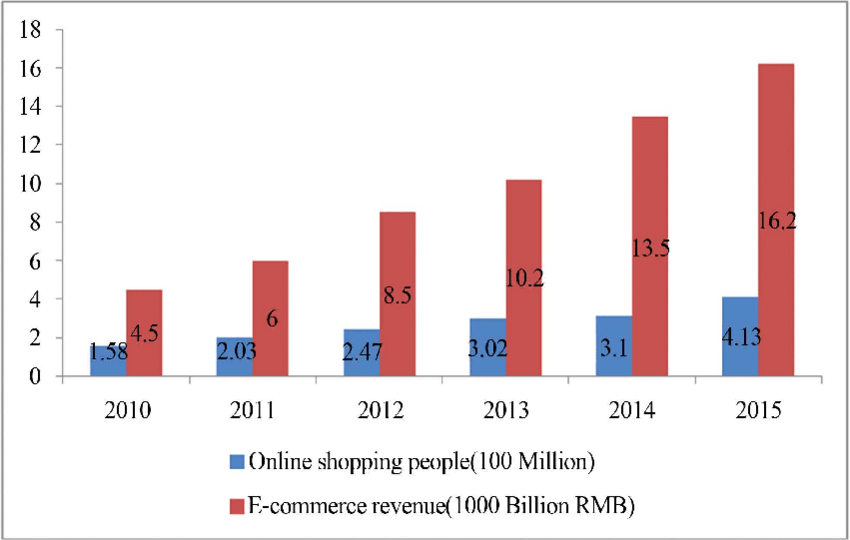
\includegraphics[width=0.6\textwidth]{Mainland E-commerce.png}
    \caption{\label{fig:Mainland E-commerce}Situation of Mainland of China E-commerce\cite{sc}}
\end{figure}

\subsection{Related Work}
Our system is called Open Mall. By referencing the design and functions of several popular e-commerce platforms and e-commerce packages, our system gathers the user-friendly features and designs altogether. To create a pleasant shopping experience for users as well as to raise the efficiency of the vendors with a well-designed, minimal but functional management interface.
\\\\
To start with, about the product explore view, Open Mall will adopt a similar way of Taobao called card view. Card view can ensure more valid information to be displayed on the application home page\cite{upx}. In addition, in order to make the users have an expectation of how to navigate the app, below the card view of a page, the interface design of Open Mall enables a blur effect to guide the user to swipe down and more products are listed as the card.
\begin{figure}[!htp]
    \centering
    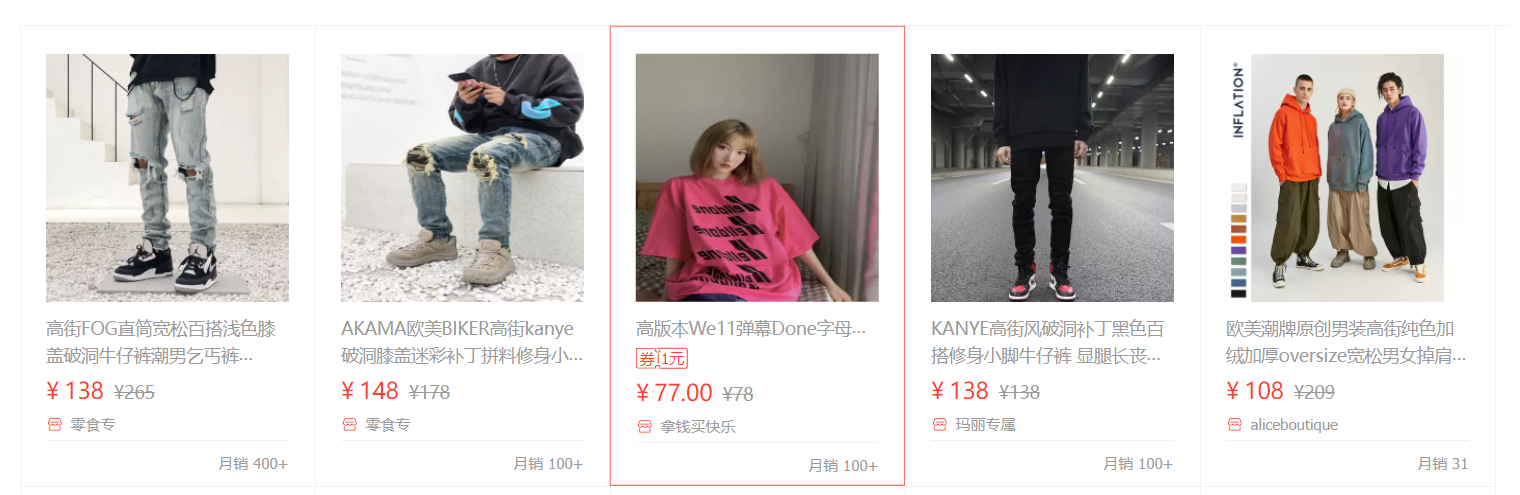
\includegraphics[width=0.6\textwidth]{card view.png}
    \caption{\label{fig:card view}Taobao's card view}
\end{figure}
\\\\
According to one of the top 10 e-commerce Design Principles for a Successful Website\cite{t10p}, "adding a searching column", the item filter is significant in improving the user experience. Hence, the function of filter products is also available in Open Mall. Users can choose the brand to control the product list displayed. Moreover, we will add the search bar at the top of the interface. By inputting the keyword, the user will get the good that they want. Just like Amazon, another reference for our platform, it has many powerful functions that provide a good user experience to users. The search function is one of them. It will give users a very simple result to directly satisfy users' needs.
\begin{figure}[!htp]
    \centering
    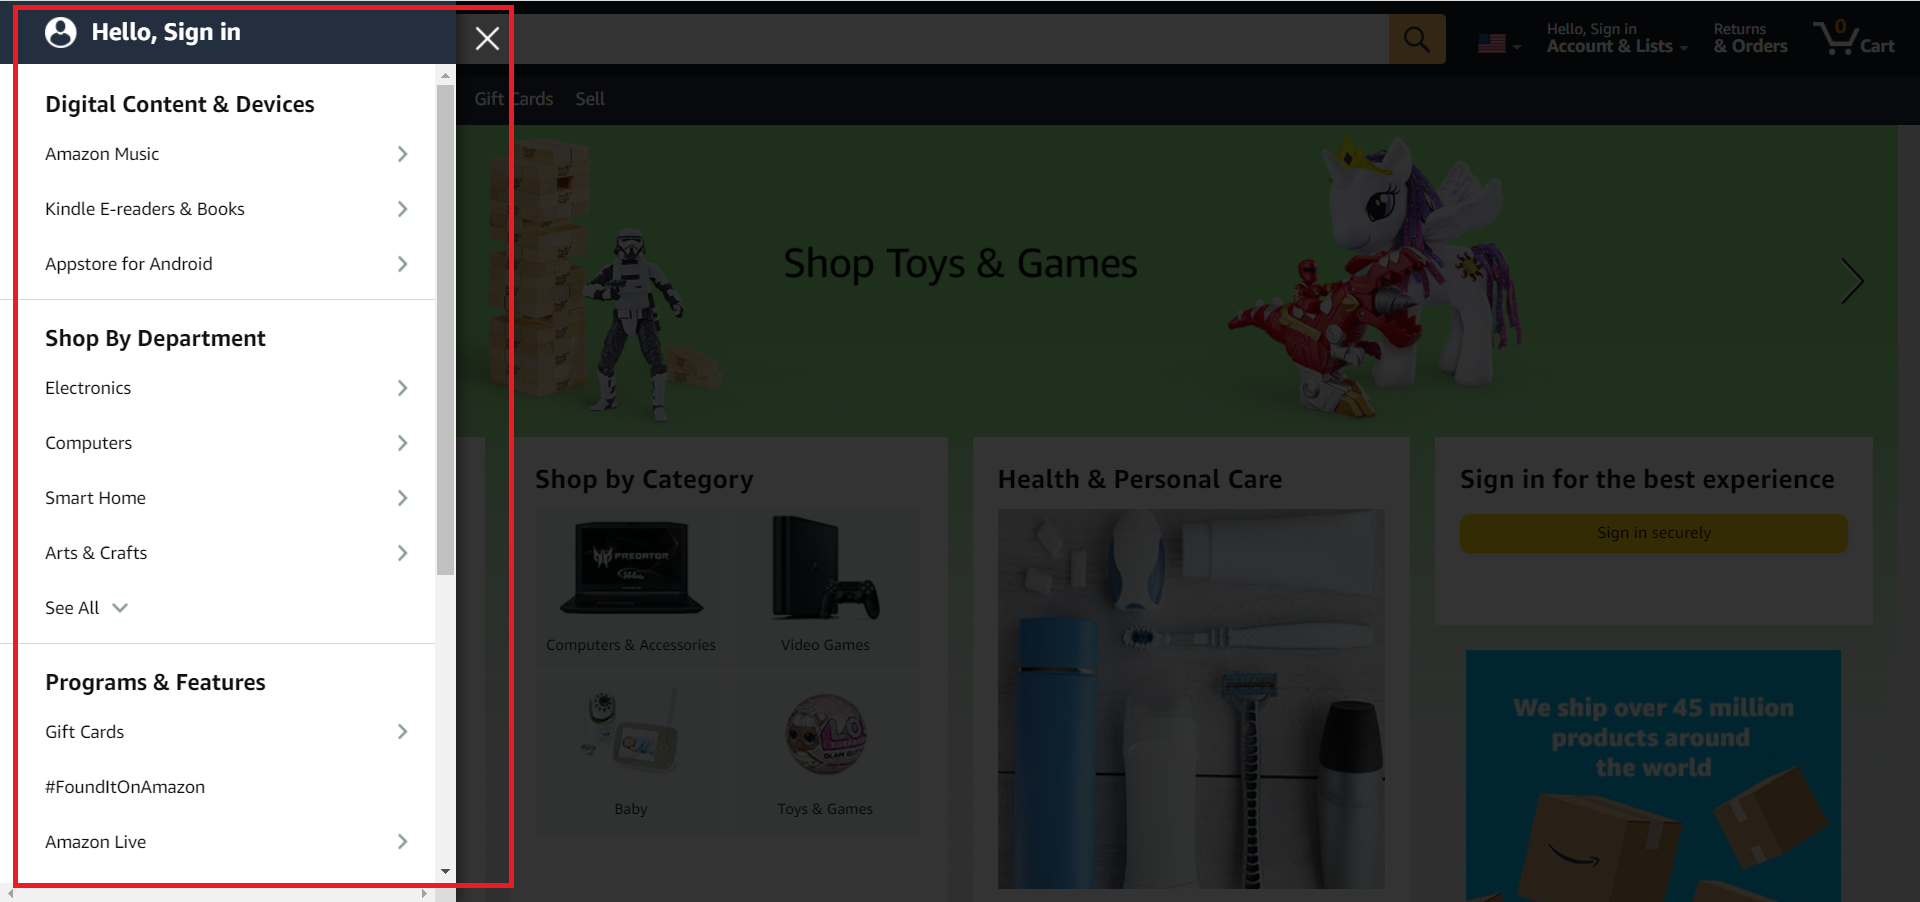
\includegraphics[width=0.9\textwidth]{Amazon filter.png}
    \caption{\label{fig:card view}Amazon's filter}
\end{figure} 
\begin{figure}[!htp]
    \centering
    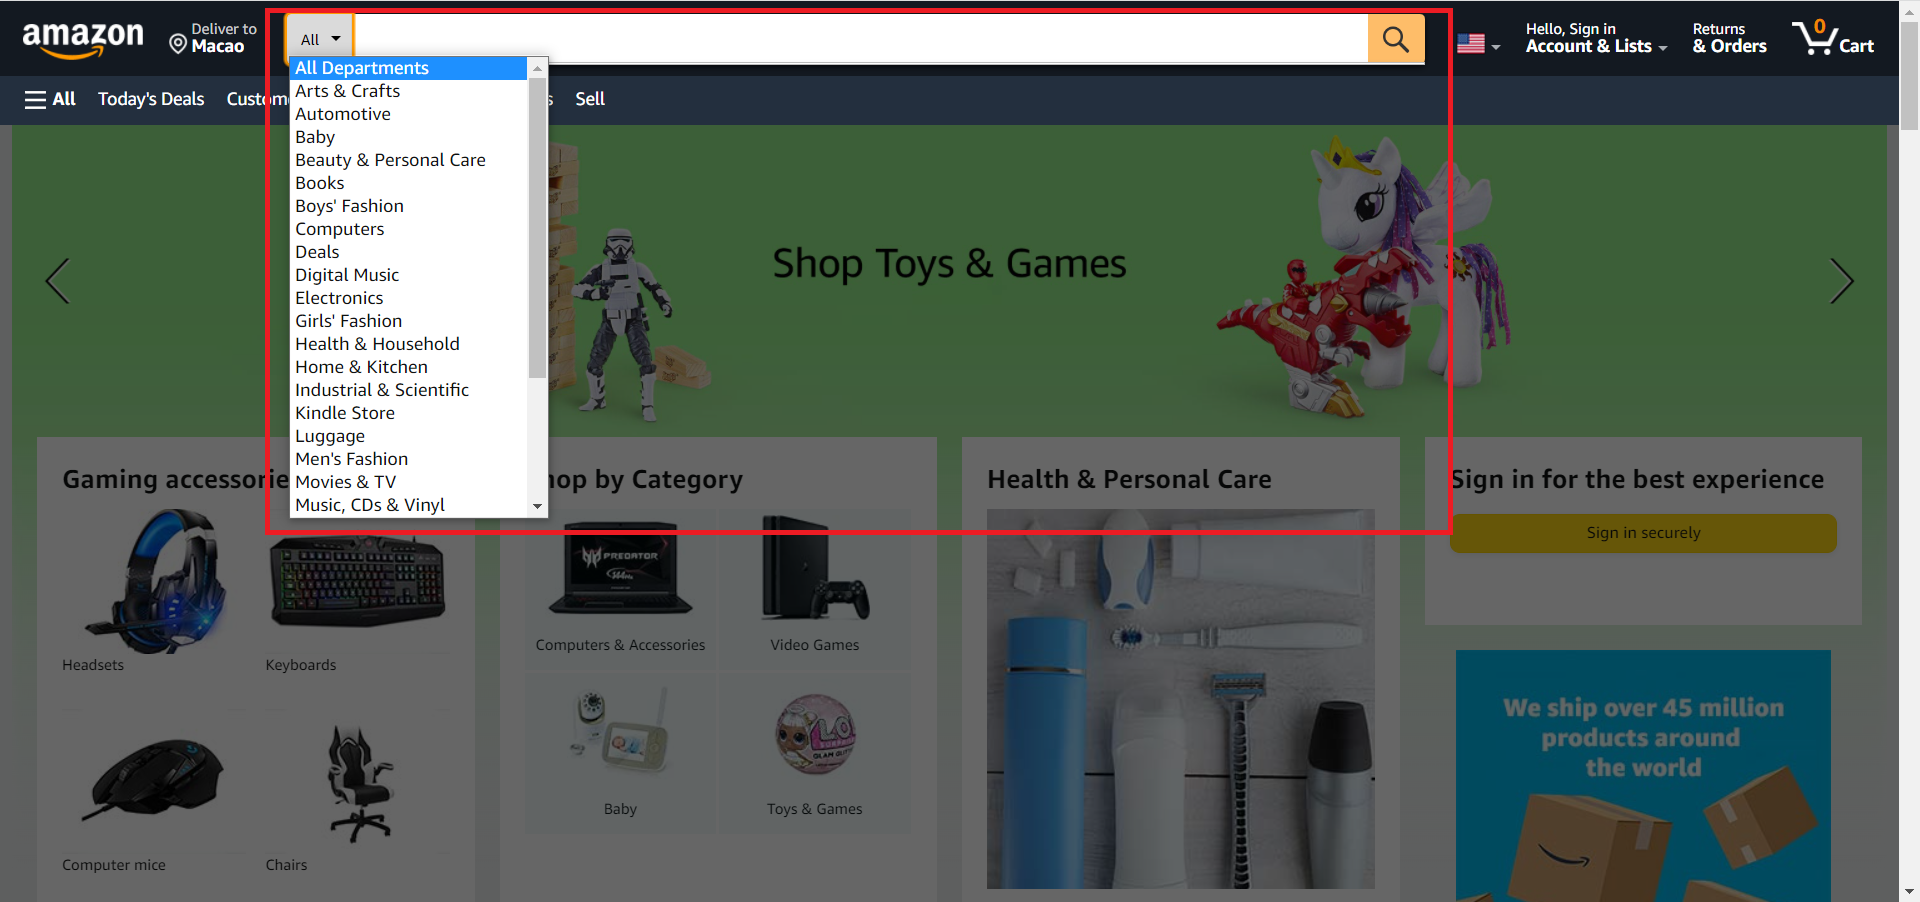
\includegraphics[width=0.9\textwidth]{Amazon search bar.png}
    \caption{\label{fig:card view}Amazon's search bar}
\end{figure} 
\\\\
The shopping cart,is an important section of the e-commerce platform. Many product functions in the e-commerce system are evolved from the existing offline products to online products, and so is the shopping cart. In offline supermarkets, we often use shopping carts. At this time, shopping carts play the following roles: convenient transportation of multiple commodities, convenient purchase of large commodities, convenient unified settlement of commodities. After moving online, the shopping cart has been given more capabilities: for users, it can save favorite items, combine prices, compare prices, categorize promotions, and offer price alerts. For platforms and merchants, shopping cart data can be collected, shopping cart marketing can be carried out, and customer unit prices can be increased\cite{shopc}. But in some e-commerce platforms for the shopping cart feature.Such as Taobao and JD, the style of the shopping cart is so complicated.In our platform, this problem will get a good solution.  
\\\\
These are just a small part of the references on our platform. In our platform,  not only a good interface design like Taobao will be provided, but also powerful and convenient functions like Amazon will be given.


\clearpage

\section{System Design}

In this chapter, we describe our database structure through the entity-relationship diagram and explain our design decisions. Besides, we will present the activity diagram to illustrate the interaction of the customers with our system.

\subsection{Data Modelling}
In this section, ER diagram and data dictionary, as well as the design concepts will be presented. 
\\\\
Figure \ref{fig:ER Diagram} shows the entities \verb|(account, address, order, product, purchase, and shopping_cart)| and the relationships among them in our online shopping system.
\begin{figure}[!htp]
    \centering
    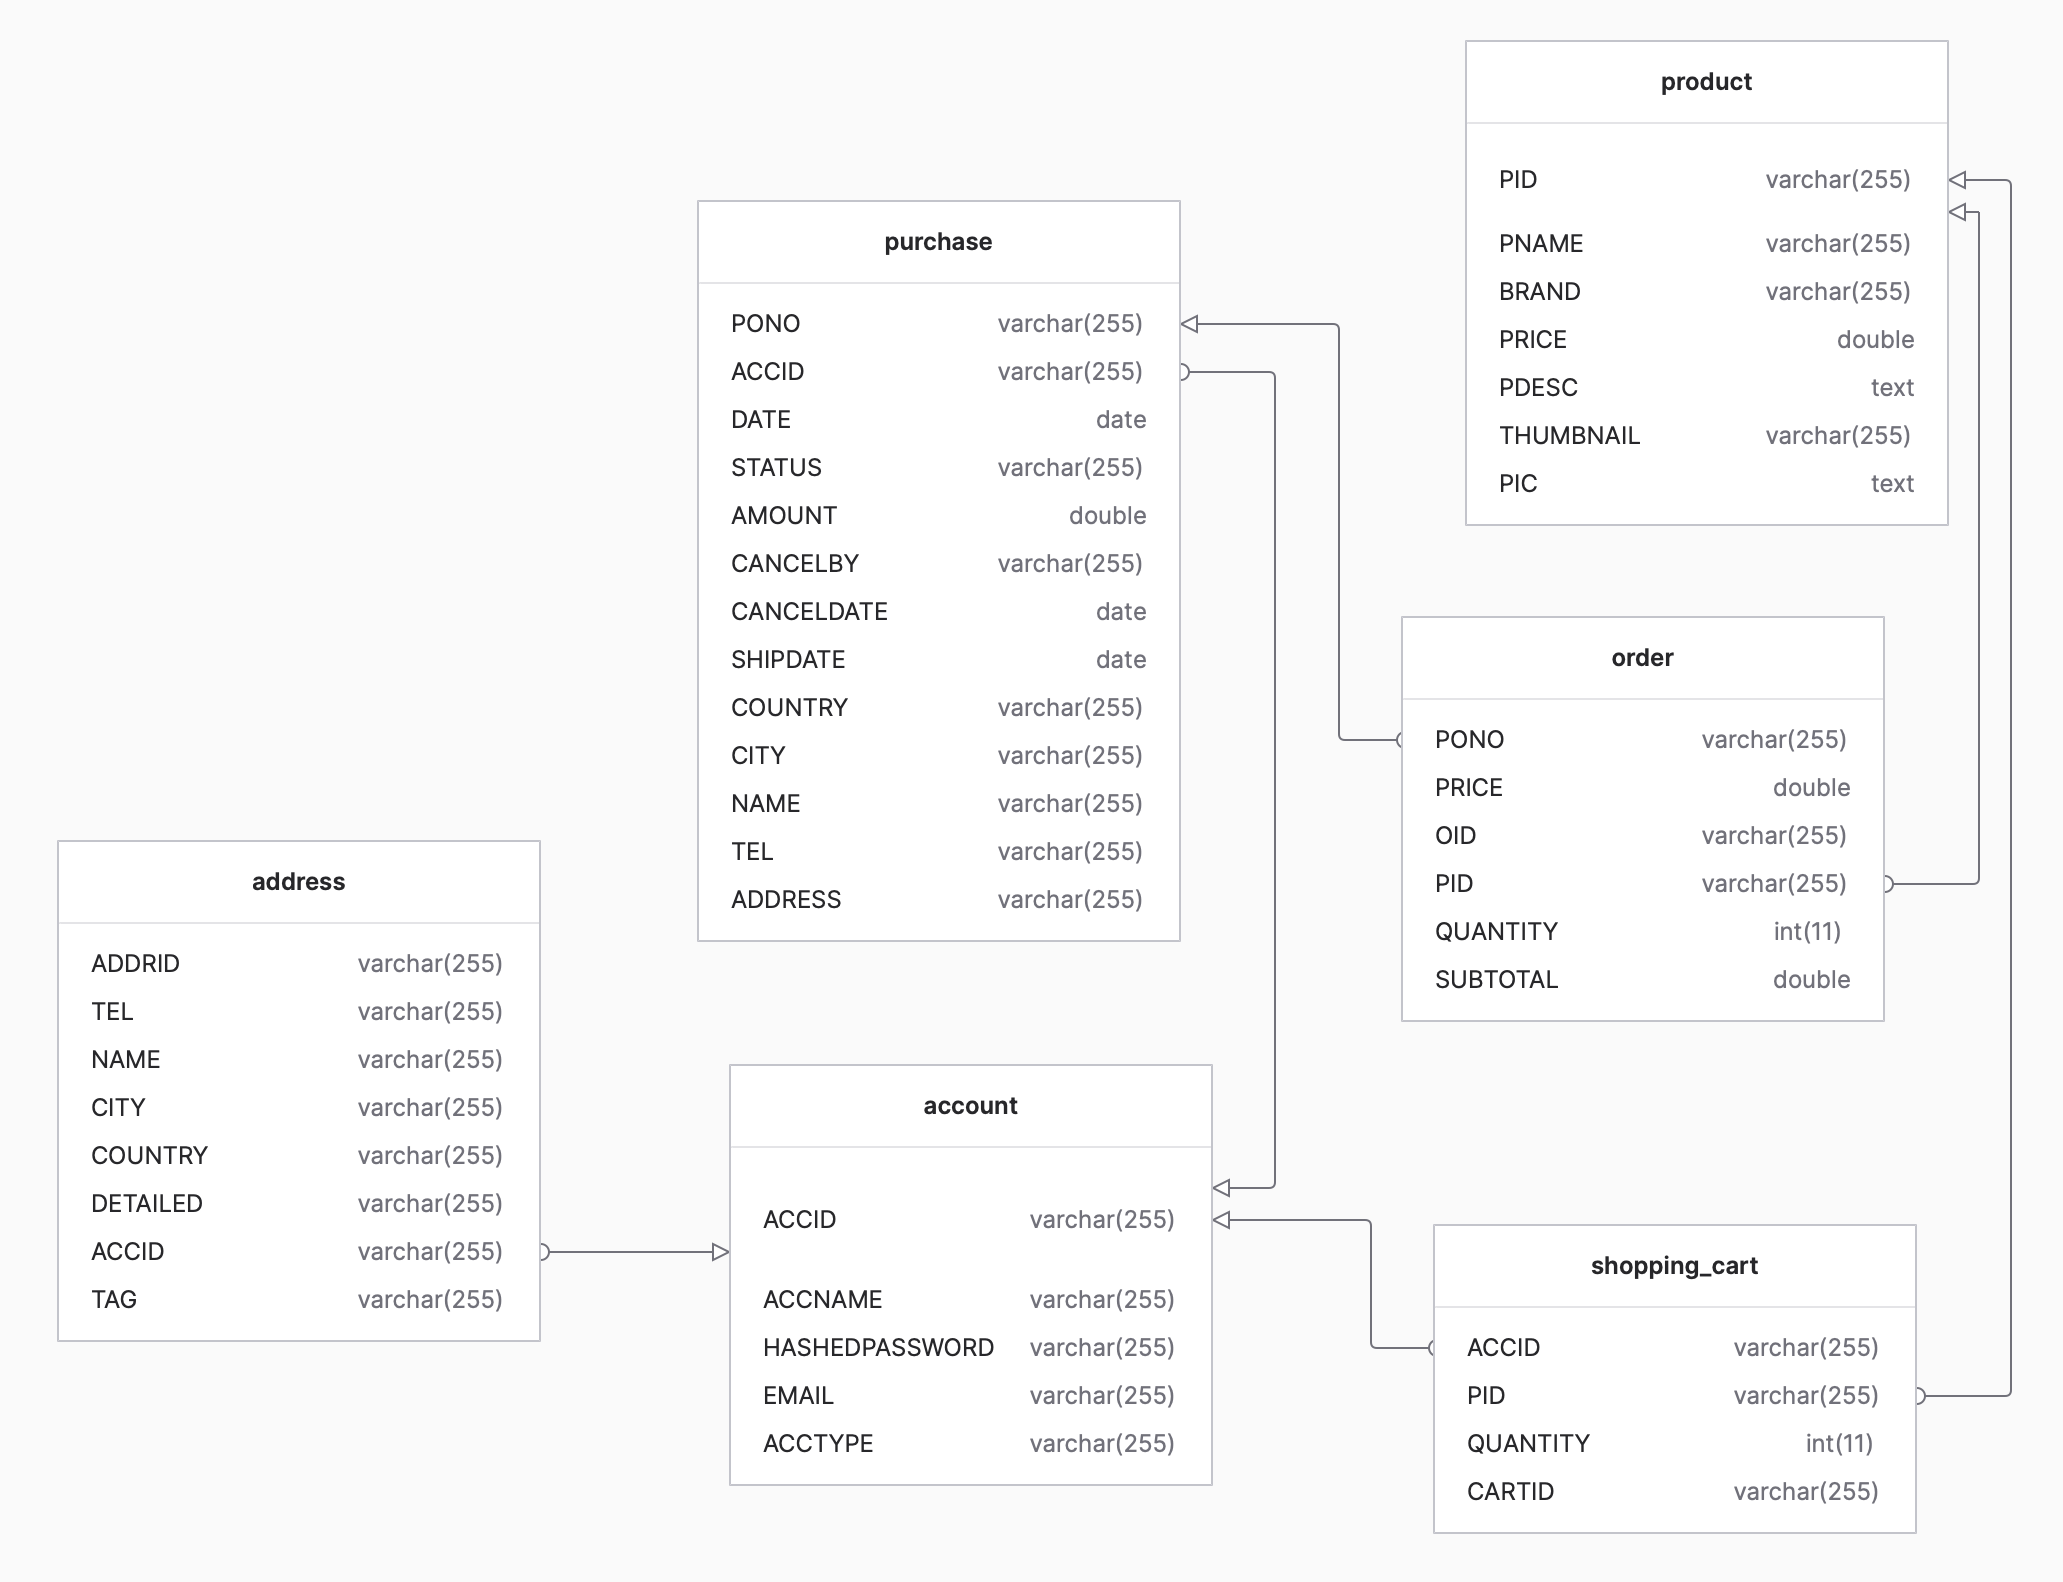
\includegraphics[width=0.9\textwidth]{ER Diagram.png}
    \caption{\label{fig:ER Diagram}ER Diagram}
\end{figure}
\\\\
The entity "account" represents the users registered in the system with account ID, account name, password in hash style, and email address. The attribute \verb|ACCTYPE| indicates the account type of the current user such as admin, vendor, or customer. 
\\\\
Considering multiple addresses are reasonable to exist under one user account, we use the entity "address" to deal with this scenario.
\\\\
The entity "product" records all the information about the goods, such as its unique product ID, product name, brand, the list unit price, all the related pictures, and a detailed description of the goods. Among them, the thumbnail image indicates the image to be shown on the store page, while all the pictures in the \verb|PIC| field will be displayed only on the product detail page
\\\\
The entity "shopping\_cart" stores the selected product and the corresponding quantity that the customers are interested in buying. Considering the price may change due to possible discounts or some other promotions in real time, the price would not be recorded in this field. Instead, it will be retrieved from the product entity via the foreign key PID. Consequently, the subtotal and total, which depend on the product price, are calculated instead of being stored.
\\\\
The entity "purchase" represents an order purchased by customers on the website with order number \verb|PONO|. This purchase list stores the account that creates this order, the date of purchase, the current order status, and the shipping date if the goods have been shipped. Information about when and by whom the order is canceled will also be recorded if it occurs. Each purchase contains one or more products.
\\\\
The entity "order" represents each of the individual products purchased. It stores the purchase price because price change should not affect the price agreed upon purchase made. As a result, the subtotal is a stored attribute because this value will not be changed once the order is created, and this design decision has a better efficiency since only a need operation is needed.
\\\\
The logical data model is listed below, giving further details on the foreign key allocation.

\begin{verbatim}
Account (ACCID, ACCNAME, HASHEDPASSWORD, EMAIL, ACCTYPE)
    Primary Key: ACCID
Address (ADDID, ACCID, TEL, NAME, CITY, COUNTRY, DETAILED, TAG)
    Primary Key: ADDID
    Foreign Key: ACCID references Account(ACCID)
Product (PID, PNAME, BRAND, PRICE, PDESC, TRUMBNAIL, PIC)
    Primary Key:PID
Shopping Cart (CARTID, ACCID, PID, QUANTITY)
    Primary Key: CARTID
    Foreign Key: ACCID references Account(ACCID)
                 PID references Product(PID)
Purchase (PONO, ACCID, date, STATUS, AMOUNT, CANCELBY, CANCELDATE, SHIPDATE, 
COUNTRY, CITY, NAME, TEL, ADDRESS)
    Primary Key: PONO
    Foreign Key: ACCID references Account(ACCID)
Order(OID, PONO, PID, PRICE, QUANTITY, SUBTOTAL)
    Primary Key: OID
    Foreign Key: PONO references Purchase(PONO)
                 PID references Product(PID)
                 
\end{verbatim}Figure \ref{fig:Data Dictionary} shows the data dictionary of all the entities and the related attributes of our system.
\begin{figure}[!htp]
    \centering
    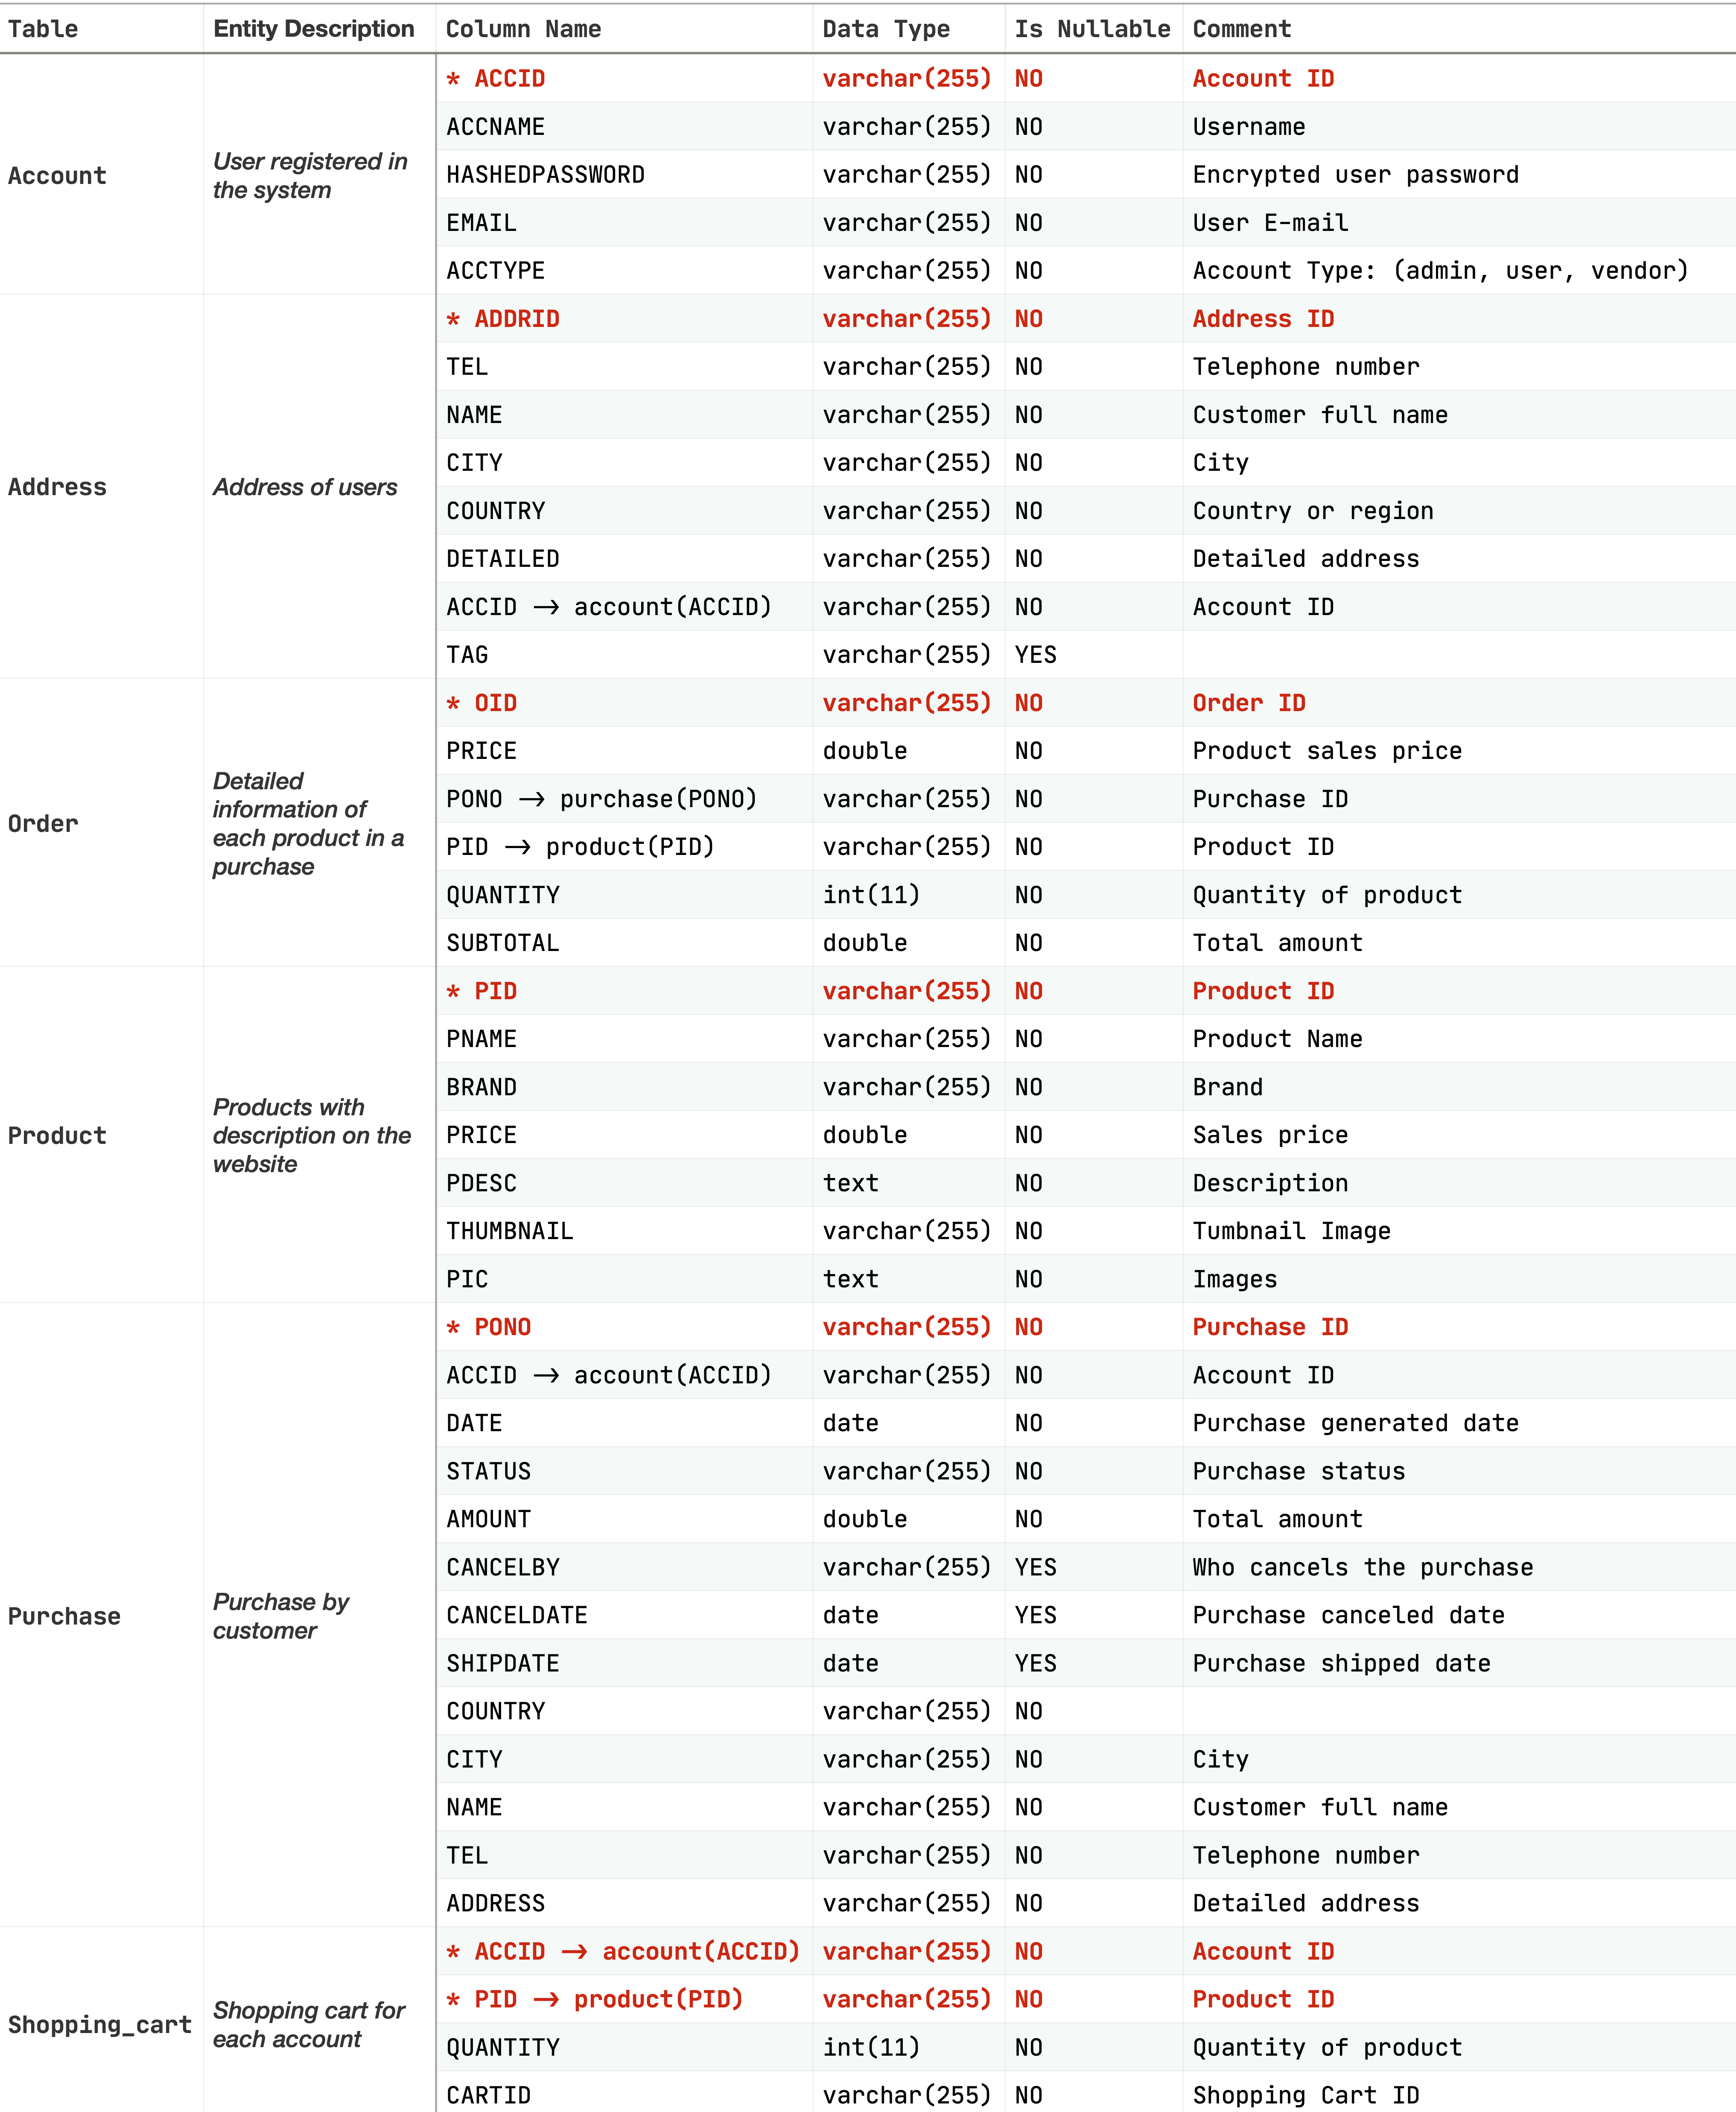
\includegraphics[width=1\textwidth]{Data Dictionary.png}
    \caption{\label{fig:Data Dictionary}Data Dictionary}
\end{figure}

\newpage
\subsection{Dynamic Modelling}
In this section, we address the interaction between the users and our system in the format of an activity diagram.
\\\\
Figure \ref{fig:Customer activity diagram} depicts the customer activity diagram that shows the various decisions paths customers can choose. Customers can only browse the product list and product detail page before login. With authentication, users are permitted to add desired items into the shopping cart. After checking the products and the quantity, the users can create an order to purchase goods. In the meantime, the shopping cart would be emptied. All the order status following can be monitored by the user. Other operations on the order like deleting before the goods are shipped is allowed.  Besides, all of the order histories can be tracked. Additionally, an accounted user can manage his/her setting such as address management and password setting. 
\begin{figure}[!htp]
    \centering
    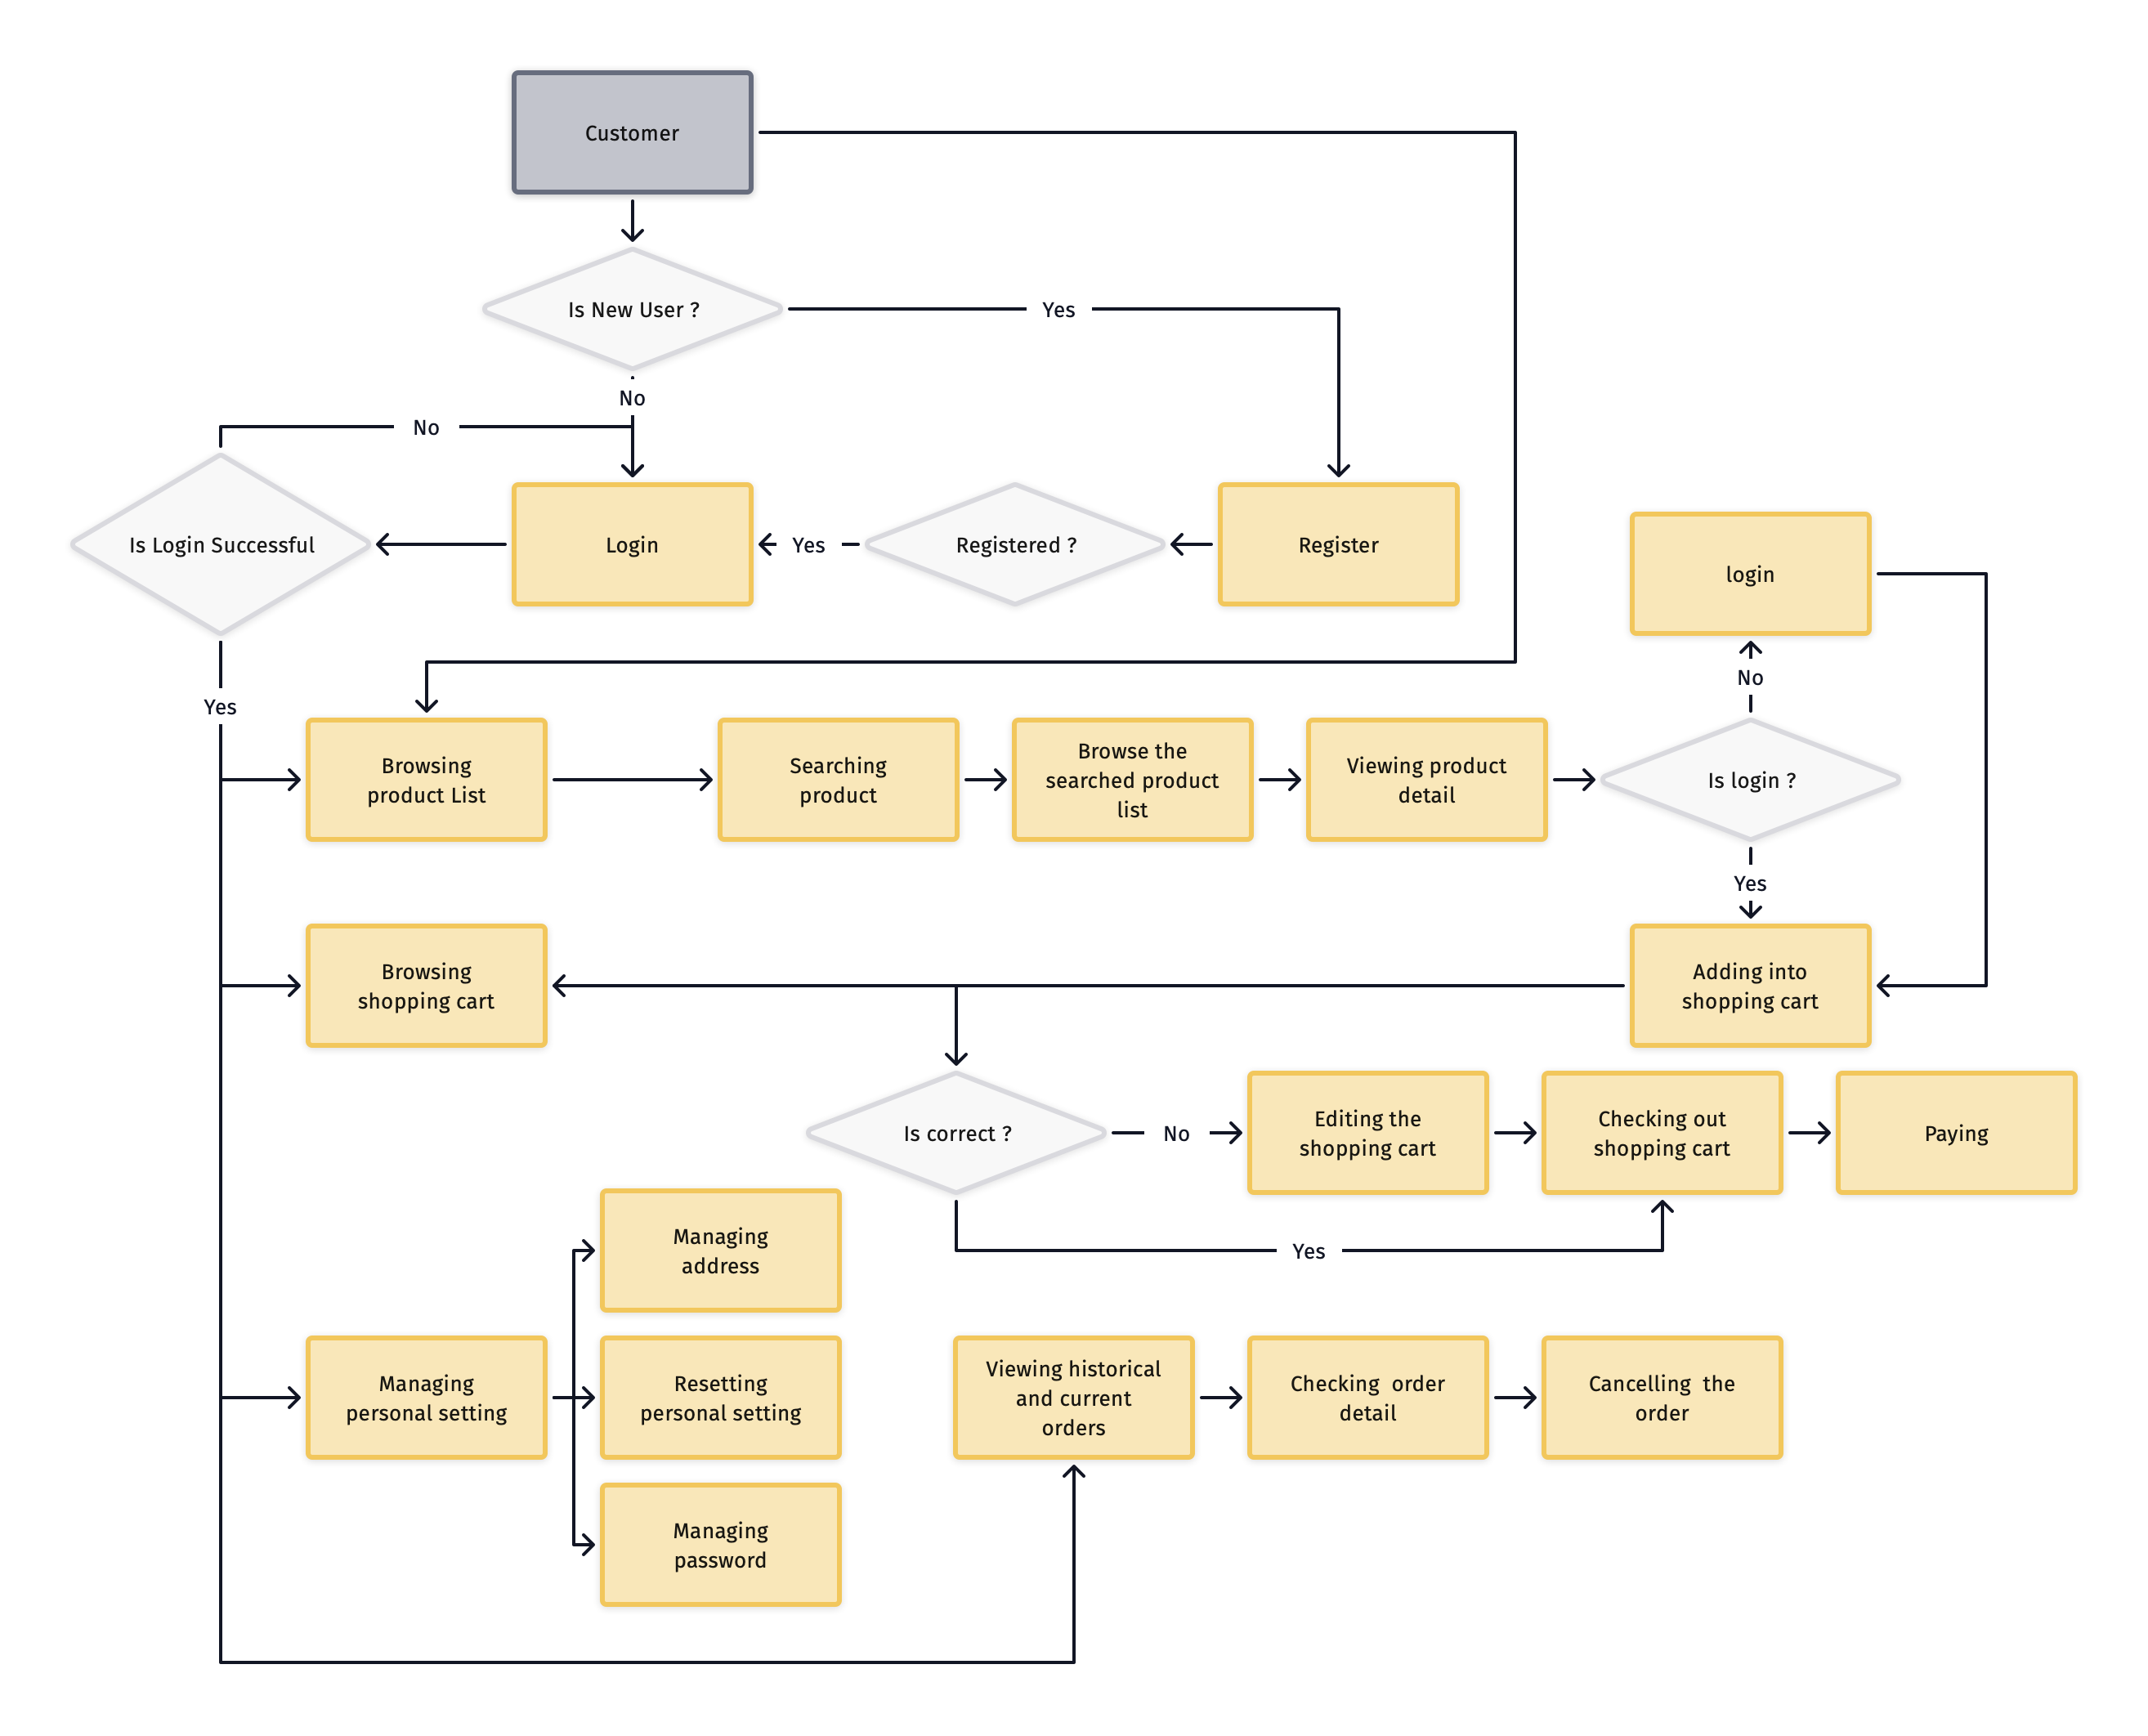
\includegraphics[width=0.9\textwidth]{Customer activity diagram.png}
    \caption{\label{fig:Customer activity diagram}Customer Activity Diagram}
\end{figure}
\\\\
Figure \ref{fig:Vendor activity diagram} illustrates vendor activity diagram that shows the various decisions paths the vendor can choose. With detailed information and uploading photographs, vendor can create new product. In the same way, vendor can modify product information in the product detail page. When browsing order list, vendor can view any order detail and mark the order status.The vendor can also cancel the order if needed. Once the product is shipped or hold, the vendor can also change the status accordingly.
\begin{figure}[!htp]
    \centering
    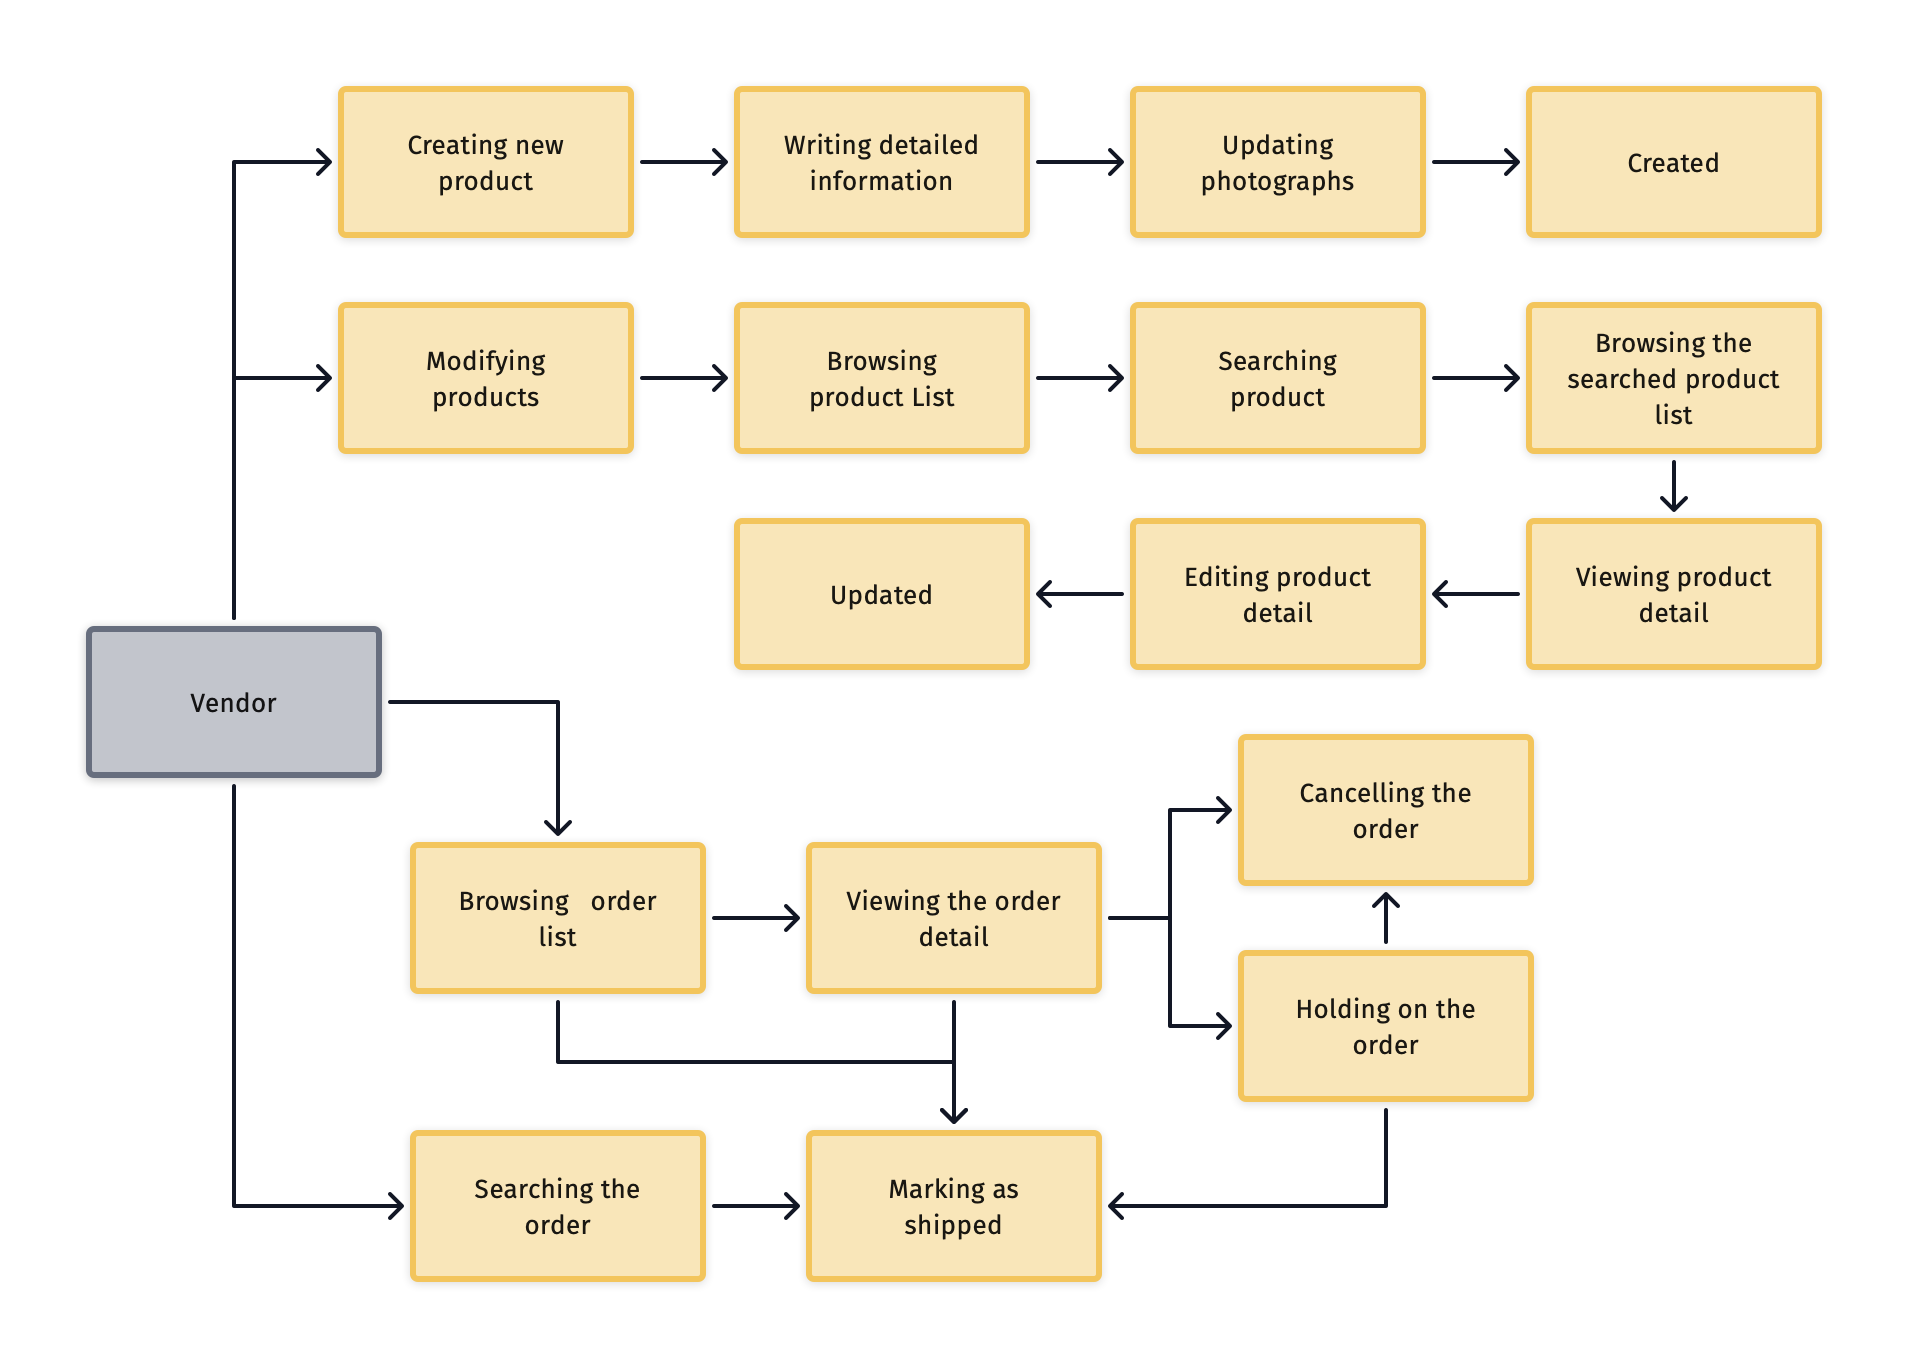
\includegraphics[width=0.9\textwidth]{Vendor activity diagram.png}
    \caption{\label{fig:Vendor activity diagram}Vendor Activity Diagram}
\end{figure}

\clearpage
\section{System Implementation}

In this section, the implementation details will be covered. In brief, we implement OpenMall with the technical stack of separation of front-end and back-end, which is a famous solution in modern web applications. Moreover, this solution is leading the era of extensive front-end. Instead of the traditional web framework rendering the webpage on the webserver, the modern approach enables the effective exchange of data via \verb|JSON| and other data-interchange formats. The rendering process of the webpage is transferred to the client's computer, which substantially saves the resources in the webserver and the transferring bandwidth.

\subsection{Architecture}

In the architectural view, OpenMall involves the separation of the front-end and back-end and the client App. Thus, the architecture is mainly in three parts, namely front-end, back-end, and client App.

\subsubsection{Front-end}

We adopted Vue.js 3.0 to implement the Single Page Application (SPA) \cite{spa} approach in front-end design. Different from the widely used version 2.0 of Vue.js, we implemented a large portion of code by using the new feature in Vue.js 3.0 like setup scripts. The lack of documentation and community support makes the implementation challengable. In addition, fewer plugins supported Vue.js 3.0 than Vue.js 2.0, which means we need to implement many infrastructures from scratch. Nevertheless, we successfully implemented our OpenMall e-commerce platform, and it meets all of the functional requirements.
\\\\
The visual design of OpenMall is implemented using Tailwind CSS. Raw and complex CSS codes have been avoided. Tailwind CSS significantly reduces the difficulty in UI and UX design. Moreover, the mobile-first design of Tailwind CSS enables effortless implementation in porting the mobile App.
\\\\
A single-page application (SPA) is a type of web application recommended by Vue.js. SPA adopted different views to display a particular page similar to the mobile App. Thus, to achieve the function of routering around the pages. We used \verb|vue-router|. The router is for controlling different logic of displaying the views by referencing the URL. Here is the declaration of part of the router links. 
\begin{listing}[!htp]
\begin{minted}{javascript}
routes: [
    { path: "/", component: Shop},
    { path: "/login", component: () => import("../views/Login.vue")},
    { path: "/signup", component: () => import("../views/Signup.vue")},
    { path: "/order", component: () => import("../views/Order.vue")},
    { path: "/order/create", component: () => import("../views/CreateOrder.vue")},
    { path: "/order/:pono", component: () => import("../views/OrderDetailed.vue")}
    // more router links omitted
]
\end{minted}
\caption{Router links}
 
\end{listing}
\leavevmode
\\\\
Considering that when users open OpenMall for the first time, it will take a lot of time to load the web application, we adopt the method of lazy loading to ensure a better user experience. The lazy loading pattern can be implemented due to lazy import under router link declaration. The view loads when the router link is clicked or the user specifies the browser's URL.
\\\\
To better support for business logic and ensuring a smooth user experience, we store all user-related data (such as account IDs and user email addresses) locally. To achieve this, we use \verb|vuex|. Vuex is a state management pattern + library for Vue.js applications. It acts as a centralized store for all components in an application, and its rules ensure that the state can only change in predictable ways \cite{vuex}. It's convenient and developed by the Vue.js community. As official support, it is widely used. Moreover, with the help of a node module named \verb|vuex-persist|, Vuex which is memory-based storage can be changed to the local storage.
\\\\
\begin{listing}[!htp]
\begin{minted}{javascript}
const vuexLocalStorage = new VuexPersist({
    key: 'vuex',
    storage: window.localStorage, // or window.sessionStorage or localForage
})
\end{minted}
\caption{Vuex Persist on Local Storage}
\label{listing:vuex-persist}
\end{listing}
\\\\
\begin{listing}[!htp]
\begin{minted}{javascript}
export default createStore({
    state: {
        userStatus: 'visitor', // active vendor visitor
        userEmail: '',
        // more attributes are ommitted ...
    },
    mutations: {
        setPrimaryAddress(state, addrId) {
            state.primaryAddress.addrId = addrId;
        },
        // more mutations are ommitted ...
    }
    plugins: [vuexLocalStorage.plugin]
})
\end{minted}
\caption{Vuex storage}
\label{listing:vuex}
\end{listing}
\leavevmode
\\\\
In addition, to communicate with the back-end, we coupled Axios in the front-end Vue.js scripts. Axios as an alternative to the original \verb|fetch| in JavaScript. It provided more function parameters and a more convenient passing of parameters with \verb|POST| requests. Detailed implementation of data communication will be introduced in the back-end section later.

\subsubsection{Back-end}

The back-end implementation includes the API server, Webserver, database. We considered FastAPI as an ideal API server that is minimally designed and can implement with Python. The Nginx Web server is for distributing web applications (front-end distribution). For the database, the open-source MariaDB is a perfect choice. This database management system balances performance and scalability. Then, we deployed the API server, Web server, and database on a single server. That server is an Elastic Hosting provided by Alibaba cloud. In deployment, we adopted a containerization solution by using Docker. Both the Nginx Webserver and MariaDB are running in two Docker containers.
\\\\
FastAPI is an API server implemented with Python. It has very high performance. To cooperate with the front-end technical stack of Vue.js, FastAPI is an appropriate choice. The FastAPI server comes with the front-end API documentation. Thus, the front-end JavaScript developer can play around with the API documentation to send requests to the back-end, which favors them in debugging and testing APIs.
\\\\
The webserver we used here is for distributing static files which need to send to the client browser. The static file is an HTML file. It is built by the Vite builder. We will introduce the static file in the next section of Integration of Front-end and Back-end. Back to the webserver, we adopted Nginx. It was the second-most widely used web server across all active sites and for the top million busiest sites. Moreover, it implemented the WSGI standard. Although in our project, the webserver is just for content distribution. The Nginx server is also a good choice.
\\\\
The most important part of the back-end is the database. We deployed the MariaDB at the beginning of our project on the cloud. We maintained a unique copy of the data. The cloud-based database makes the further development of different computers of our members easier. The choice of database is MariaDB, which is the community-supported version of MySQL. It has excellent performance and a variety of community support. As for the core part of our project, it is essential to be consistent. Especially for the table schema. If there is inconsistency, the development and debugging process will be in big trouble. In the meanwhile, alternating the table schema during the development process is fatal. In the data modelling process, there was a fault that we failed to consider the changes in user addresses. Then we designed the \verb|Purchase| table with only the user address ID foreign key. Finally, we noticed the failure of the design. So we need to rewrite several lines of code. And this led to several bugs in many lines of code related to business logic. Hence, we need to consider all of the situations in the data modeling process.

\subsubsection{MVVM Structure}

MVVM consists of Model, View, and ViewModel. The Model layer represents the data model, and the business logic of data modification and operation can also be defined in the Model; View represents the UI component, which is responsible for transforming the data model into UI for display. ViewModel is a Synchronize View and Model objects.
\begin{figure}[!htp]
    \centering
    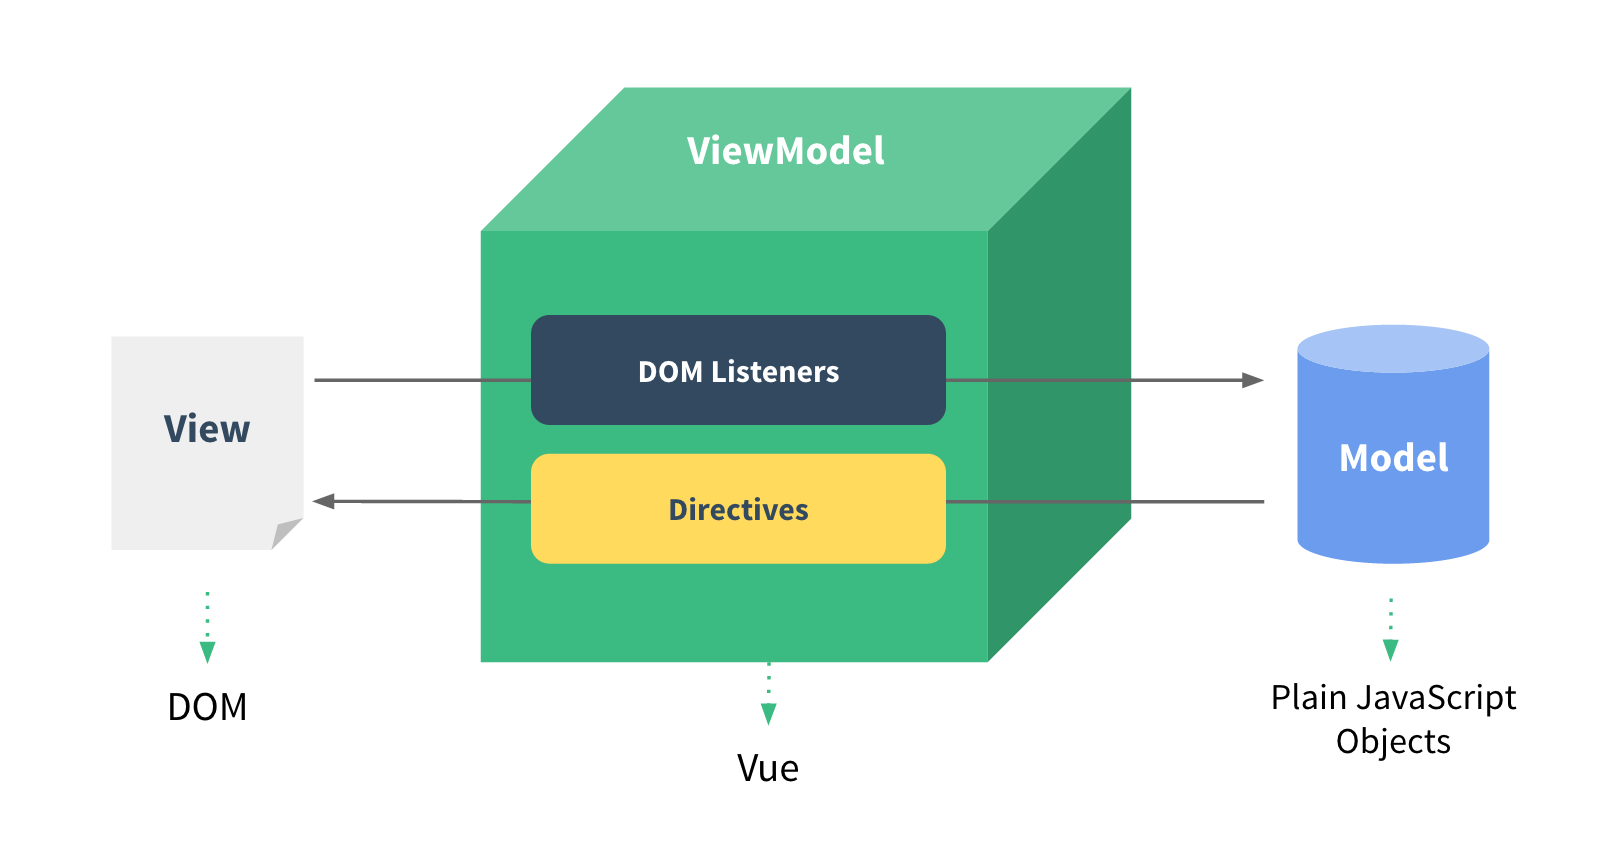
\includegraphics[width=0.7\textwidth]{mvvm.png}
    \caption{\label{fig:mvvm}MVVM structure}
\end{figure}
\\\\
Under the MVVM architecture, there is no direct connection between the View and the Model, but the interaction is through the ViewModel. The interaction between the Model and the ViewModel is bidirectional, so the changes of the View data will be synchronized to the Model, and the changes of the Model data will be synchronized. It will also immediately react to the View.
\\\\
ViewModel connects the View layer and Model layer through two-way data binding, and the synchronization between View and Model is completely automatic without human intervention, so developers only need to pay attention to business logic, do not need to manually manipulate the DOM, do not Need to pay attention to the synchronization of data state, complex data state maintenance is completely managed by MVVM.

\subsubsection{Integration of Front-end and Back-end}

Apart from the traditional webpage, the server renders all of the user data of a specific user and sends the rendered webpage to the client browser. Modern web applications adopted the separation of front-end and back-end methods similar to mobile applications. That is, when a client user requests the web application, the static file server (we implemented using Nginx) sends a webpage (application more accurately) to the client browser. Till now, the client browser can run the web application locally without fetching data. If the scenario is data-driven, like our OpenMall project, the web application should have data communication with the API server. The web application works with fetching and sending data from or to the API server. And the process of data communication using EDI is mainly the integration.
\\\\
For the front-end, we adopted a node module (NodeJS Library) named \verb|form-data| to work with \verb|v-model| in Vue.js to implement the form data upload (like register form, address creation form). While for the back-end, we created a class (as seen in listing \ref{listing:formdata}) inherits \verb|fastapi.BaseModel| to get the submission from the front-end. Then the instance will be handled by the Model of the database.

\begin{listing}[!htp]
\begin{minted}{python}
class RegisterData(BaseModel):
    email: str
    hashed_password: str
\end{minted}
\caption{User registration class}
\label{listing:formdata}
\end{listing}

\subsubsection{Resolving the issue of Cross-origin resource sharing}

JavaScript and web programming have grown by leaps and bounds over the years, but the same-origin policy still remains. This prevents JavaScript from making requests across domain boundaries and has spawned various hacks for making cross-domain requests. Corss-origin resource sharing (CORS)\cite{cors} introduces a standard mechanism that can be used by all browsers for implementing cross-domain requests. The spec defines a set of headers that allow the browser and server to communicate about which requests are (and are not) allowed. When the front-end web application communicates with the back-end, CORS restricts the communication process. Thus, we need to specify the request header and tell the server and client browser that it should be allowed for all of the essential sites when using our system.
\\\\
To resolve the CORS issue, we need to configure the FastAPI using middleware. To achieve this, the backend must have a list of "allowed origins". The core code is shown in listing \ref{listing:cors}.
\begin{listing}[!htp]
\begin{minted}{python}
from fastapi import FastAPI
from fastapi.middleware.cors import CORSMiddleware

app = FastAPI()

origins = [
    "http://localhost",
    "http://localhost:8080",
]

app.add_middleware(
    CORSMiddleware,
    allow_origins=origins,
    allow_credentials=True,
    allow_methods=["*"],
    allow_headers=["*"],
)
\end{minted}
\caption{Enable CORS middleware in FastAPI}
\label{listing:cors}
\end{listing}

\subsubsection{API}

An application that separates the front-end and back-end needs API as a bridge to exchange EDI (in our project is JSON format). Commonly speaking, developers can deploy the database server and API server on a different server. That is for saving performance. If the scale of a business is large, load balancing will be considered using reverse proxy and Redis. However, we considered quick-response a bit more significant than scalability. Thus, we deployed the database server and API server in a single cloud server. When the API server retrieves data from the database server, the response can be at the millisecond level due to the localhost socket transmission.
\\\\
The implementation of API is in Python, and front-end uses Axios to request the API. That is the fundamental process of an API request. For instance, to implement the API for retrieving the data in a cart of a particular user in the back-end. The Python code is shown in listing \ref{listing:apiImpl}.
\begin{listing}[!htp]
\begin{minted}{python}
@app.get("/api/cart/products/{accId}")
def get_cart_by_id(accId: str):
    from db.database import get_all_products_in_cart
    return get_all_products_in_cart(accId)
\end{minted}
\caption{Example back-end API implementation}
\label{listing:apiImpl}
\end{listing}

\leavevmode
\\\\
The corresponding API request implemented in the front-end by JavaScript is shown

\begin{listing}[!htp]
\begin{minted}{javascript}
const query =
    "http://" + config.apiServer + ":" + config.port
    + "/api/cart/products/" + accId.value;
    
axios.get(query).then((res) => {
  // lines of codes omitted
});
\end{minted}
\caption{Example front-end API request}
%\label{listing:3}
\end{listing}

\subsection{Project structure}

We maintained the OpenMall project on GitHub repository \verb|Ex10si0n/ISI|. In this section, the project file structure will be introduced. 

\begin{minted}{python}
Open-Mall/                             (cont.)
    OpenMall/                          src/
        Assets.xcassets                    App.vue
        Info.plist                         components/
        OpenMallApp.swift                  config.ts
        Views/                             main.ts
    OpenMall.xcodeproj/                    router/
isi-api/                                       router.ts
    README.md                              store/
    api.py                                     countries.ts
    db/                                        store.ts
        database.py                        views/
        img/                                   About.vue
        password_validator.py                  AddressList.vue
        settings.py                            Cart.vue
    environment.yml                            ChangePassword.vue
    init/                                      CreateAddress.vue
        environment.yml                        CreateOrder.vue
        schema.sql                             CreateProduct.vue
    start.sh                                   Login.vue
isi-web/                                       Manage.vue
    README.md                                  Order.vue
    dist/                                      OrderDetailed.vue
        assets                                 Product.vue
        favicon.ico                            Profile.vue
        index.html                             Search.vue
    index.html                                 Shop.vue
    package.json                               Signup.vue
    public/                                    UpdateProduct.vue
        favicon.ico                       README.md
\end{minted}

\subsubsection{iOS App}

\verb|isi-app/| is the source code of the Xcode project of OpenMall iOS App, the entry of the main program is \verb|OpenMallApp.swift|, the views are under \verb|Views/|. The implementation of the iOS App is driven by \verb|SwiftUI|, which is for rendering the structure and layouts of the application. See more detailed information in the implementation of the iOS App section.

\subsubsection{Back-end API server}

\verb|isi-api| is the implementation of back-end API server. The main entry of back-end is \verb|api.py|. We grouped all codes and files related to the database into \verb|db/|. The model for executing SQL command is in \verb|db/database.py|. The product image data is stored under \verb|db/img/|. The helper method of hashing and validating passwords is encapsulated in \verb|db/password_validator.py|. Settings of database server IP is in \verb|db/settings.py|. Under the \verb|init/| folder, there are environment specifications and database table schema. These two files are necessary for the initial deployment of OpenMall. In addition, the shell scripting shortcut \verb|start.sh| is for running the FastAPI server.

\subsubsection{Front-end Vue.js Project}
The front-end Vue.js Project is built based on the boilerplate provided by \verb|Ex10si0n/quick-starts|, which is a GitHub repository maintained by Steve. The quick-start template is a Vite project and he added TypeScript, Vuex, Vue-router, and Tailwind CSS support. For the front-end structure, the \verb|dist/| folder contains the static file built by the Vite builder, this file is uploaded to the server and Nginx static file server distributes it to the client browser. \verb|package.json| is the package environment specification by the Yarn package manager. Under the \verb|src/| folder, \verb|App.vue| is the main entrance of the front-end project. Vue components are under \verb|src/components/|, and the Vue-router views are under \verb|src/views/|. The code to implement the router and its related functions are under \verb|src/router/|. Local storage implementation and persist user login status are maintained under \verb|src/store/|. Plus, the file \verb|src/main.ts| contains the main entrance of the package import, and the file \verb|src/config.ts| contains the configuration of the back-end API server IP and port.

\subsection{Containerization deployment}

The back-end database server and front-end static file server of the OpenMall project is deployed on a webserver to provide services. We adopted the approach of containerization deployment to make the deployment process lite. 
\\\\
Docker is an open-source platform for developing, shipping, and running applications. It can separate the applications from the infrastructure so the developer can deliver software quickly.
\\\\
For the back-end database server, we pull the MariaDB Image from Docker Hub and run it by command:

\begin{listing}[!htp]
\begin{minted}{bash}
docker run --name isi-mariadb
    -e MYSQL_ROOT_PASSWORD=root
    -p 3306:3306
    -d mariadb:10.3
    --log-bin
    --binlog-format=MIXED
\end{minted}
\caption{Shell script for running MariaDB in Docker}
%\label{listing:3}
\end{listing}

\leavevmode
\\\\
For the front-end static file distribution server, we pull the Nginx Image and run it by command:

\begin{listing}[!htp]
\begin{minted}{bash}
docker run --name isi-static
    -e TZ="Asia/Shanghai"
    -d -p 3000:80
    -v /home/ubuntu/isi-web/dist/:/usr/share/nginx/html
    nginx
\end{minted}
\caption{Shell script for running Nginx in Docker}
%\label{listing:3}
\end{listing}

\subsection{Product List and Product Detail Display}

\subsubsection{Product List: card view template}
Vue uses an HTML-based template syntax that allows the developer to declaratively bind the rendered DOM to the underlying component instance's data. All Vue templates are syntactically valid HTML that can be parsed by spec-compliant browsers and HTML parsers.
\\\\
Under the hood, Vue compiles the templates into highly-optimized JavaScript code. Combined with the reactivity system, Vue is able to intelligently figure out the minimal number of components to re-render and apply the minimal amount of DOM manipulations when the app state changes. \cite{template}
\\\\
OpenMall adopted a card view on the design of the product list. In the desktop version, the product card layout is similar to Taobao, which is the waterfall column layout. To implement the card view, there is a card view template. And the data get from the API are filled into the template by the Vue.js template. Listing \ref{listing:card-template} shows the Vue.js template code of the card template.
\\\\
To shorten the display length of the product description. We use \verb|split()| to truncate the number of words and it allows only eight words in each of the card view of the product.

\begin{listing}[!htp]
\begin{minted}{html}
<img class="py-0 rounded-t-lg object-cover lg:h-80 lg:w-80" 
    :src="product.thumbnail"/>
<div class="px-5 py-2 pb-5">
    <h3 class="font-semibold tracking-tight text-gray-900 text-md">
      {{ product.pname }}
    </h3>
    <h3 class="text-sm font-semibold tracking-tight text-gray-500">
      {{ product.pdesc.split(" ").slice(0, 8).join(" ") }}
    </h3>
    <div class="flex items-center mt-2.5 mb-5">
      <span class="bg-blue-100 text-blue-800 text-xs font-semibold mr-2 
          px-2.5 py-0.5 rounded">{{ product.brand }}</span>
    </div>
    <div class="flex items-center justify-between">
      <span class="font-bold text-gray-700 text-md">HK\${{ product.price }}</span>
    </div>
  </div>
</div>
\end{minted}
\caption{Card Template}
\label{listing:card-template}
\end{listing}

\subsubsection{Product Detail Display}

In the product's detailed display, there is not only the essential information about the product but also the address selection button. When the user clicks it, the primary address selection page will pop up and the user can change the current address to another. After that, the user clicks the back button, then he or she will be redirected back to the previous browsed product. The function of redirect back is implemented by the \verb|viewingProduct| in the browser's local storage. The backlink in the primary address selection page is dynamic by filling the ID of the viewing product that is stored in the local storage, as shown in listing \ref{listing:viewProduct}.

\begin{listing}[!htp]
\begin{minted}{html}
<router-link v-if="viewingProduct !== ''" :to="'/product/' + viewingProduct">
  <!-- Back button style omitted -->
</router-link>
\end{minted}
\caption{Backlink to current viewing product}
\label{listing:viewProduct}
\end{listing}

\leavevmode
\\\\
Moreover, we adopted a carousel view of images (see Figure \ref{fig:carousel}). The carousel component is provided by NaiveUI. The implementation of the related code is under \verb|src/components/Carousel.vue|. The code is shown in listing \ref{listing:carousel}
\begin{figure}[!htp]
    \centering
    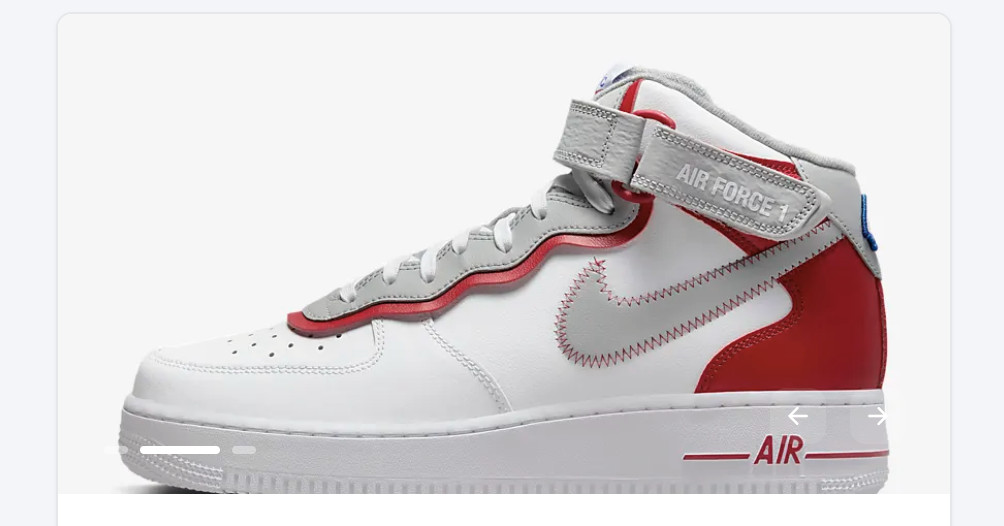
\includegraphics[width=0.3\textwidth]{Carousel.png}
    \caption{\label{fig:carousel}Carousel view of images}
\end{figure}


\begin{listing}[!htp]
\begin{minted}{html}
<n-carousel show-arrow autoplay>
  <img v-for="p in pic" class="carousel-img h-auto" :src="p"/>
  <!-- template for button is omitted -->
  <template #dots="{ total, currentIndex, to }">
    <ul class="custom-dots">
      <li
          v-for="index of total"
          :class="{ ['is-active']: currentIndex === index - 1 }"
          :key="index"
          v-on:click="to(index - 1)"
      ></li>
    </ul>
  </template>
</n-carousel>
\end{minted}
\caption{Component of carousel image view}
\label{listing:carousel}
\end{listing}


\subsection{Product Search, Filtering, and Sorting}
\subsubsection{Product Search}
This function allows customers to search products by product names and enable the vendor to search products by names and IDs. Whether the searching keywords are names or IDs, this function is generally achieved by integrating the front-end and the back-end. 
\\\\
The front-end part of this function is to track an input searching keyword, send a get request to the server with this keyword, and handle the response from the server. To be more specific, after clicking the searching box in \verb|Shop.vue|, the users jump to \verb|Search.vue|. In \verb|Search.vue|, the input searching keyword is tracked by the \verb|v-model| variable named \verb|content|. And get requests are performed with the tracked value of this variable by Axios in \verb|search| function. Since there are two different types of users (customers and the vendor), two different URLs are used in these get requests. The get request with the URL \verb|"/api/search/name/" + content.value| is used for customers and vendors. And an additional get request with the URL \verb|"/api/search/id/" + content.value| is also used for the vendor. After getting the response from the server, the result is pushed into the reactive array named \verb|products|, and \verb|v-for| directive is used to access and show each element in this array (see Listing \ref{listing: The search function in the front end}).
\\\\
\begin{listing}[!htp]
\begin{minted}{javascript}
const search = () => {
// The process of getting images and filtering the products with the selected brand
  let searchResult1 = true
  let searchResult2 = true
  axios
    .get("http://" + config.apiServer + ":" + config.port +
      "/api/search/name/" + content.value)
    .then((res) => {
      if (res.data.status === 'success') {
        const productList = res.data.products;
        productList.forEach((product: ProductState) => {
          products.push(product as ProductState);
        })
      } else if (res.data.status === 'none') {
        searchResult1 = false
        if (store.state.userStatus != 'vendor') {
          result.value = "None"
        }
      }
      if (store.state.userStatus === 'vendor') {
        axios
          .get("http://" + config.apiServer + ":" + config.port +
          "/api/search/id/" + content.value)
          .then((res) => {
            if (res.data.status === 'success') {
              searchResult2 = true;
              products.push(product as ProductState);
            } else if (res.data.status === 'none') {
              searchResult2 = false;
              if (!searchResult1 && !searchResult2) {
                result.value = "None"
              }
            }
          })
      }
    })
}
\end{minted}
\caption{The search function in the front end}
\label{listing: The search function in the front end}
\end{listing}The back-end part of this function is to handle the get request from the front-end, get data from the database, and send a response to the front-end. Specifically, the sent requests are handled by the route handlers \verb|@app.get(‘/api/search/name/{pname}’)| and \verb|@app.get(‘/api/search/id/{pid}’)| in the file \verb|api.py|. And these two route handlers call the method \verb|get_products_by_name(name: str)| and the method \verb|get_product_by_id(id: str)| separately in the file database.py. In these two methods, the matched data is selected from the database (see Listing \ref{listing: The two methods about searching products in the database.py}). It is worth mentioning that the \verb|LIKE| operator is used in SQL to be able to select products by blur product names. After being selected from the database, the corresponding data is put in a dictionary object named \verb|product|. Every \verb|product| object is appended to a list which is put in a dictionary object \verb|playload| and returned as the result from the front-end. 
\\\\
\begin{listing}[!htp]
\begin{minted}{python}
def get_products_by_name(name: str):
    playload = {'status': '', 'products': []}
    try:
        connection = create_connection()
        with connection:
            with connection.cursor() as cursor:
                sql = "SELECT * FROM `product` WHERE `PNAME` LIKE %s"
                cursor.execute(sql, ('%' + name + '%',))
                result = cursor.fetchall()
                if (len(result) == 0):
                    playload['status'] = 'none'
                    return playload
                else:
                    playload['status'] = 'success'
                    for row in result:
                        product = {
                            'pid': row['PID'],
                            # The other attributes in this row 
                            # is similar to this one.
                        }
                        playload['products'].append(product)
                    return playload
    except:
        playload['status'] = 'error'
        return playload
def get_product_by_id(id: str):
    # The code in this method is similar to the previous method, 
    # except the following SQL statement.
    sql = "SELECT * FROM `product` WHERE `PID`=%s"
    cursor.execute(sql, (id,))
\end{minted}
\caption{The two methods about searching products in the database.py}
\label{listing: The two methods about searching products in the database.py}
\end{listing}Based on the understanding of the structure of this function, the problem met in the implementation of this function can be explained in the following part. To be more specific, the problem is how to identify the none results of two responses. Since there are two get requests with two different URLs and these two get requests are asynchronous callbacks, the responses of these get requests may not come in the order of the code. Thus, it is difficult to determine a time point to identify whether the two results in the responses both are none. To solve this problem, the get request with the URL \verb|"/api/search/id/" + content.value| is embedded in the \verb|.then()| method of another Axios get request with the URL \verb|"/api/search/name/"|\\\verb| + content.value|. Thus, when the response of the embedded get request is obtained, the response of the outer one is sure to have been got already. In this situation, the two results can be checked by the \verb|searchResult1| and \verb|searchResult2| separately in \verb|if| conditional statements so that whether there are two none results can be identified (see Listing \ref{listing: The search function in the front end}).
\newpage
\subsubsection{Filtering}
This function allows users to filter the product list by brand. This function is implemented mainly in the front end. To be more specific, a drop-list is provided for users to select the brand. And the brand chosen is tracked by a \verb|v-model| variable \verb|brandFilter| through an arrow function. The value of this variable is used in the \verb|.filter()| method to filter the products with the matched brand from the reactive array \verb|products|. Subsequently, the brand value in the drop-list is updated by a \verb|.map()| method according to the brands of the remaining products in the array (see Listing \ref{listing: Filtering}). 
\begin{listing}[!htp]
\begin{minted}{javascript}
const products_brands = computed(() => {
  return products.map((product) => product.brand);
});

const filtered_products = computed(() => {
  if (brandFilter.value === "all") {
    // The part of sorting products by price is omitted.
    return products;
  } else {
    // The part of sorting products by price is omitted.
    return products.filter((product) => product.brand === brandFilter.value);
  }
}
});
\end{minted}
\caption{Filtering}
\label{listing: Filtering}
\end{listing}\\\\
The brand filter can also be used with the function of searching keywords for products. To be more specific, after getting the responses, a \verb|if| conditional statement is used so that only the products with the matched brands can be pushed into the displayed list (see Listing \ref{listing: Filtering brand in the function of searching}).
\begin{listing}[!htp]
\begin{minted}{javascript}
const search = () => {
  // The part for searching is omitted.
  if (res.data.status === 'success') {
    const productList = res.data.products;
    productList.forEach((product: ProductState) => {
      if (product.brand === brandFilter.value || brandFilter.value == "all") {
        products.push(product as ProductState);
      }
    })
  }
}
\end{minted}
\caption{Filtering brand in the function of searching}
\label{listing: Filtering brand in the function of searching}
\end{listing}
\newpage
\subsubsection{Sorting}
This function allows the users to sort the products by price. The products can be sorted from high to low prices and from the opposite way. This function is implemented mainly in the front end. To be more specific, a drop-list is provided for users to select the way of sorting. A \verb|v-model| variable \verb|sortPrice| tracks the choice. And according to the value of this variable, different arrow functions are put as the parameter in the \verb|.sort()| method to sort the elements in the array (see Listing \ref{listing: Sorting}).
\begin{listing}[!htp]
\begin{minted}{javascript}
const filtered_products = computed(() => {
  // The part of filtering products by brands is omitted.
  if (sortPrice.value === "default") {
    return products;
  } else if (sortPrice.value === "l2h") {
    return products.sort((a, b) => a.price - b.price);
  } else if (sortPrice.value === "h2l") {
    return products.sort((a, b) => b.price - a.price);
  }
});
\end{minted}
\caption{Sorting}
\label{listing: Sorting}
\end{listing}
\subsection{Image Handling}
This part explains how to handle the images, including uploading, storing, displaying, and deleting images. 
\\\\
To upload the images, three steps need to be actualized, including obtaining the input images, sending a post request with these images, and receiving these images in the back end. To be more specific, an \verb|input| tag is used to get the images, and in this \verb|input| tag, the attribute \verb|accept = “image/*”| in this tag limits the types of the uploaded file and prevents the program from throwing some errors caused by the unexpected file type (Listing \ref{listing: The input tag for uploading image}). Subsequently, these input files are caught by \verb|event.target.files| or \verb|event.dataTransfer.files| when the \verb|input| tag is changing (Listing \ref{listing: The input files are tracked as the value of variables}). After that, the grabbed files are appended to a \verb|FormData| object with the same name \verb|‘images’|, and this \verb|FormData| object is contained in a post request with the headers \verb|‘Content-Type’: ‘multipart/form-data’| (Listing \ref{listing: The post request for uploading images}). Finally, this \verb|FormData| object is handled by an async method with the input parameter for a list of \verb|UploadFile| also named \verb|‘images’| in \verb|api.py| (Listing \ref{listing: Receive images in api.py}).
\begin{listing}[!htp]
\begin{minted}{html}
<input accept = "image/*" type = "file" v-on:change = "onFileChange" multiple/>
\end{minted}
\caption{The input tag for uploading images}
\label{listing: The input tag for uploading image}
\end{listing}
\begin{listing}[!htp]
\begin{minted}{javascript}
const onFileChange = (event) => {
  const files = event.target.files || event.dataTransfer.files;
  for (let i = 0; i < files.length; i++) {
    img.push(files[i])
  }
}
\end{minted}
\caption{The input files are tracked as the value of variables}
\label{listing: The input files are tracked as the value of variables}
\end{listing}
\begin{listing}[!htp]
\begin{minted}{javascript}
const createProduct = () => {
  const formData = new FormData();
  formData.append("images", thumbnailImage.value)
  for (let i = 0; i < img.length; i++) {
    formData.append('images', img[i])
  }
  const queryImage = "http://" + config.apiServer + ":" + config.port 
  + "/api/image/upload"
  axios.post(queryImage, formData, {
    headers: {
      'Content-Type': 'multipart/form-data'
    }
  }).then()
  // Other parts are omitted.
}
\end{minted}
\caption{The post request for uploading images}
\label{listing: The post request for uploading images}
\end{listing}
\begin{listing}[!htp]
\begin{minted}{python}
@app.post('/api/image/upload')
async def upload_image(images: List[UploadFile]):
\end{minted}
\caption{Receive images in api.py}
\label{listing: Receive images in api.py}
\end{listing}
\newpage
\leavevmode
\\\\
To store images, two steps need to be actualized, including storing the images in the \verb|img| folder and storing the names of the images in the database. To be more specific, after the images are got in the \verb|api.py|, these images are written in files under the folder \verb|img| (Listing \ref{listing: Save images in the img folder}). Moving on to another part, the names of thumbnails are stored as the value of the attribute \verb|THUMBNAIL| in the entity \verb|Product|. The names of detailed pictures are joined as an entire string with semicolons and stored as the value of the attribute \verb|PIC| in the entity (Figure \ref{fig:Example for storing names for images}). The reason for not storing the images in the database directly is that the images have bigger sizes than other data in general, so they can waste plenty of space in the database and significantly reduce the performance of the database.
\begin{listing}[!htp]
\begin{minted}{python}
for image in images:
    path = os.path.join(fpath, 'img/' + image.filename)
    with open(path, 'wb') as f:
        f.write(image.file.read())
\end{minted}
\caption{Save images in the img folder}
\label{listing: Save images in the img folder}
\end{listing}
\begin{figure}[!htp]
    \centering
    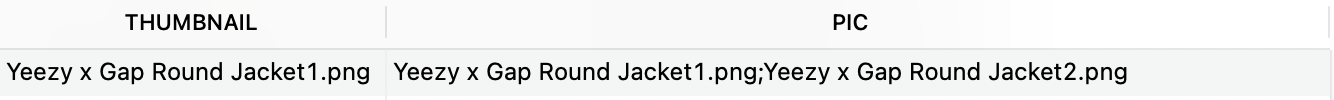
\includegraphics[width=1\textwidth]{Example for storing names for images.png}
    \caption{Example for storing names for images}
    \label{fig:Example for storing names for images}
\end{figure}
\\\\
To display images, there are two different ways to display saved or unsaved images. To be more specific, for the saved images, image names got from the database are used as a part of the URL \verb|"/api/img/" + |\\\verb|pic| (Listing \ref{listing: Build the URLs for getting images}). These URLs are used as attribute \verb|src| in \verb|img| tag. These URLs are handled by the corresponding route handler, and the images are returned through \verb|FileResponse| by this route handler (Listing \ref{listing: Return images through FileResponse}). To display multiple images, an additional component \verb|n-carousel| needs to be imported from Naive UI to have a slide effect for showing these images. Moving on to the unsaved images, the input images can be read as URLs by the \verb|FileReader|. And these URLs are used to update the attribute \verb|src| in image tags so the image can be previewed before saving (Listing \ref{listing: Get the URLs for unsaved images}). 
\begin{listing}[!htp]
\begin{minted}{javascript}
axios
  .get(
    "http://" + config.apiServer + ":" + config.port + "/api/product/" + 
    route.params.pid
  )
  .then((res) => {
    // Other parts are omitted.
    const json = res.data.product;
    product.pic = [];
    json.pic.split(";").forEach((pic: string) => {
      product.pic.push(
        "http://" + config.apiServer + ":" + config.port + "/api/img/" + pic
      );
    });
  })
\end{minted}
\caption{Build the URLs for getting images}
\label{listing: Build the URLs for getting images}
\end{listing}
\begin{listing}[!htp]
\begin{minted}{python}
@app.get("/api/img/{filename}")
async def root(filename: str):
    return FileResponse(os.path.join(fpath, 'img/' + filename))
\end{minted}
\caption{Return images through FileResponse}
\label{listing: Return images through FileResponse}
\end{listing}
\begin{listing}[!htp]
\begin{minted}{javascript}
for (let i = 0; i < img.length; i++) {
  let reader = new FileReader()
  reader.readAsDataURL(img[i])
  reader.onload = function() {
    let dataURL = reader.result as string
    imgList.value.push(dataURL)
  }
}
\end{minted}
\caption{Get the URLs for unsaved images}
\label{listing: Get the URLs for unsaved images}
\end{listing}
\\\\
To delete images, there are also two different ways to delete saved or unsaved images. To be more specific, for the saved images, the route handler uses the names of the images to find the images and removes the images from the \verb|img| folder (Listing \ref{listing: Remove images from the img folder}). For the unsaved images, the string of names of images is split into a list. The deleted images are found by the data URL, and the name of the images are popped from the list. After that, the updated list is joined into a string, and the deleted images are not uploaded at all. 
\begin{listing}[!htp]
\begin{minted}{python}
@app.post('/api/image/delete')
async def delete_image(deleteImageData: DeleteImageData):
    path = os.path.join(fpath, 'img/' + deleteImageData.picName)
    os.remove(path)
\end{minted}
\caption{Remove images from the img folder}
\label{listing: Remove images from the img folder}
\end{listing}
\newpage
\subsection{Password Security}
This part explains three aspects of password security – password strength, storing hash values of passwords, and verifying passwords. 
\\\\
For password strength, the passwords must contain at least six characters, one digit, and one capital letter. To check whether the password meets the strength requirement, the length of the password is checked first. Subsequently, every character in this password is checked to identify whether it is a digit or a capital letter. If all the requirements are satisfied, the password can be stored in the database. Otherwise, an alert will be popped up to remind the user to change the password (Listing \ref{listing: Check password strength}).
\begin{listing}[!htp]
\begin{minted}{javascript}
const checkPassword = () => {
  let numberFlag = false
  let capitalFlag = false
  if (password.value.length >= 6) {
    for (var char of password.value) {
      for (var digit of ['0', '1', .. '8', '9']) {
        if (char == digit) {
          numberFlag = true
          break
        }
      }
      for (var letter of ['A', 'B', .. 'Y', 'Z']) {
        if (char == letter) {
          capitalFlag = true
          break
        }
      }
    }
    if (numberFlag == true && capitalFlag == true) {
      return true
    } else {
      alert("At least one digit\nAt least one capital letter")
      return false
    }
  } else {
    alert("At least 6 characters")
    return false
  }
}
\end{minted}
\caption{Check password strength}
\label{listing: Check password strength}
\end{listing}
\\\\
Passwords are saved in hash values in the database, which can prevent the database staff from knowing the users’ passwords and performing some actions without permission. To achieve this function, the passwords with the corresponding \verb|ACCID|s are merged as hash values by the hash algorithm \verb|sha256()| of the library \verb|hashlib| (Listing \ref{listing: Get the hash value of the password}).
\begin{listing}[!htp]
\begin{minted}{python}
# database.py
password_validator.hash(password, accId)

# password_validator.py
def hash(password, password_encoding_salt):
    hashed = hashlib.sha256((password + password_encoding_salt).encode('utf-8'))
    .hexdigest()
    return hashed
\end{minted}
\caption{Get the hash value of the password}
\label{listing: Get the hash value of the password}
\end{listing}
\newpage
\leavevmode
\\\\
In terms of verifying passwords, the email is used to select the specific account information and get the \verb|ACCID| and the \verb|HASHEDPASSWORD|. The \verb|ACCID| is merged with the given password as a new hash value that is compared with the \verb|HASHEDPASSWORD|. If they are the same, the password is verified successfully (Listing \ref{listing: Verify the password}).
\begin{listing}[!htp]
\begin{minted}{python}
given_hashed_password = password_validator.hash(password, result['ACCID'])
if given_hashed_password == result['HASHEDPASSWORD']:
    playload['status'] = 'success'
\end{minted}
\caption{Verify the password}
\label{listing: Verify the password}
\end{listing}
\subsection{Purchase Order Processing}
This part explains the control for changing purchase order status. This function is achieved on two levels – the outer level is used to check the availability for this changing status action, and the inner level is a common method \verb|update_status()| to change the status. To be more specific, the present purchase status is checked in the \verb|if| conditional statement. If the present status is the required status, the status can be updated. Otherwise, updating is rejected (Listing \ref{listing: The control for changing purchase order status}).
\begin{listing}[!htp]
\begin{minted}{python}
def update_status(pono: str, status: str):
    # Other parts are omitted.
    sql = "UPDATE `purchase` SET `STATUS` = %s WHERE `PONO` = %s"
    cursor.execute(sql, (status, pono))
    connection.commit()
def cancel_purchase(accType: str, pono: str):
    # Other parts are omitted.
    if(status == 'pending' or status == 'hold'):
        update_status(pono, 'cancelled')
        playload['status'] = 'success'
        return playload
    else:
        playload['status'] = 'forbidden'
        return playload
def ship_purchase(pono: str):
    # Other parts are omitted.
    if(status == 'pending'):
        update_status(pono, 'shipped')
        playload['status'] = 'success'
        return playload
def hold_purchase(pono: str):
    # Other parts are omitted.
    if(status == 'pending'):
        update_status(pono, 'hold')
        playload['status'] = 'success'
        return playload
def unhold_purchase(pono: str):
    # Other parts are omitted.
    if(status == 'hold'):
        update_status(pono, 'shipped')
        playload['status'] = 'success'
        return playload
\end{minted}
\caption{The control for changing purchase order status}
\label{listing: The control for changing purchase order status}
\end{listing}
\clearpage
\subsection{UI Design}
For UI design, we picked the Tailwind CSS framework instead of regular CSS to render our front-end pages. Tailwind CSS is a functional class-first CSS framework based on the idea of tools that are smaller and more flexible than components. This idea would rather simply use classes than achieve personalizing on the basis of components to ensure flexibility and facilitate custom components.
\\\\
It means, first of all, Tailwind CSS has incredible performance due to its ultra-small file size. In development mode, every possible classes are generated in order to avoid waiting for the build process to finish. While once Tailwind CSS goes into production mode,  all classes not used with the PurgeCSS tool will be purged , which is achieved by searching the project file for the name of the class and keeping only those that are used. 
\\\\
With regular CSS, custom classes need to be written for each element on the page. While this provides better control, writing custom classes takes a lot of time: we have to add the class in HTML, create it in CSS, and write out each property in long form. Then we have to wait for the CSS to build to see the results - and if we need to make more changes, we need to rebuild every time, which can take a few seconds and interrupt our flow.
\\\\
Tailwind CSS removes these extra steps and provides a simple, straightforward development experience when styling elements. We can see the element we want to style, add the required properties using shorthand, and change quickly without waiting for CSS bundles. So as long as we focus on one place, we do not have to switch to different files frequently, and the whole process feels smooth.
\\\\
Referring to the usage of Tailwind CSS, the style declaration is plugged into the class of an HTML element. It also supports selectors like \verb|hover:| which refers to the style when the user hovers their mouse on that element. In this example \ref{listing:tailwindcss}, it describes a style of a pagination selector. The selector has two buttons for the jump to the next and previous page. The two buttons are arranged in the same row. So we used the \verb|grid-cols-2| layout. It can divide a row into two columns. Moreover, the other style declarations such as \verb|bg|, \verb|border|, and \verb|h-6| are respectively background color, border style, and box height.
\begin{listing}[!htp]
\begin{minted}{html}
<div class="mt-2 grid grid-cols-2 gap-2">
    <button 
        v-on:click="prevPage" 
        class="hover:bg-slate-100 hover:shadow-none border 
               text-blue-500 rounded h-6 shadow"
    >Previous</button>
    <button 
        v-on:click="nextPage" 
        class="hover:bg-slate-100 hover:shadow-none border 
               text-blue-500 rounded h-6 shadow"
    >Next</button>
</div>
\end{minted}
\caption{Usage of Tailwind CSS}
\label{listing:tailwindcss}
\end{listing}

\leavevmode
\\\\
Considering all of the above, Tailwind CSS can provide better semantic understanding and better responsive layout to design our interface conveniently and efficiently.
\\\\
In the early days of web design, pages were built to target particular screen sizes. If the user had a larger or smaller screen than the designer expected, results ranged from unwanted scrollbars to overly long line lengths, and poor use of space. As more diverse screen sizes became available, the concept of responsive web design (RWD) appeared \cite{responsive}, a set of practices that allows web pages to alter their layout and appearance to suit different screen widths, resolutions, etc. That is, a single HTML code can be rendered into the target device with an adaptive layout that can fit each of the screen sizes with the most suitable appearance.
\\\\
OpenMall is designed as a mobile-first web application. However, to have better support for desktop browsers, we adopted the feature of a flexible box (a solution of responsive layout) in Tailwind CSS. So the desktop version of OpenMall has an elegant interface involving a waterfall content list, as seen in Figure \ref{fig:waterfall}

\begin{figure}[!htp]
    \centering
    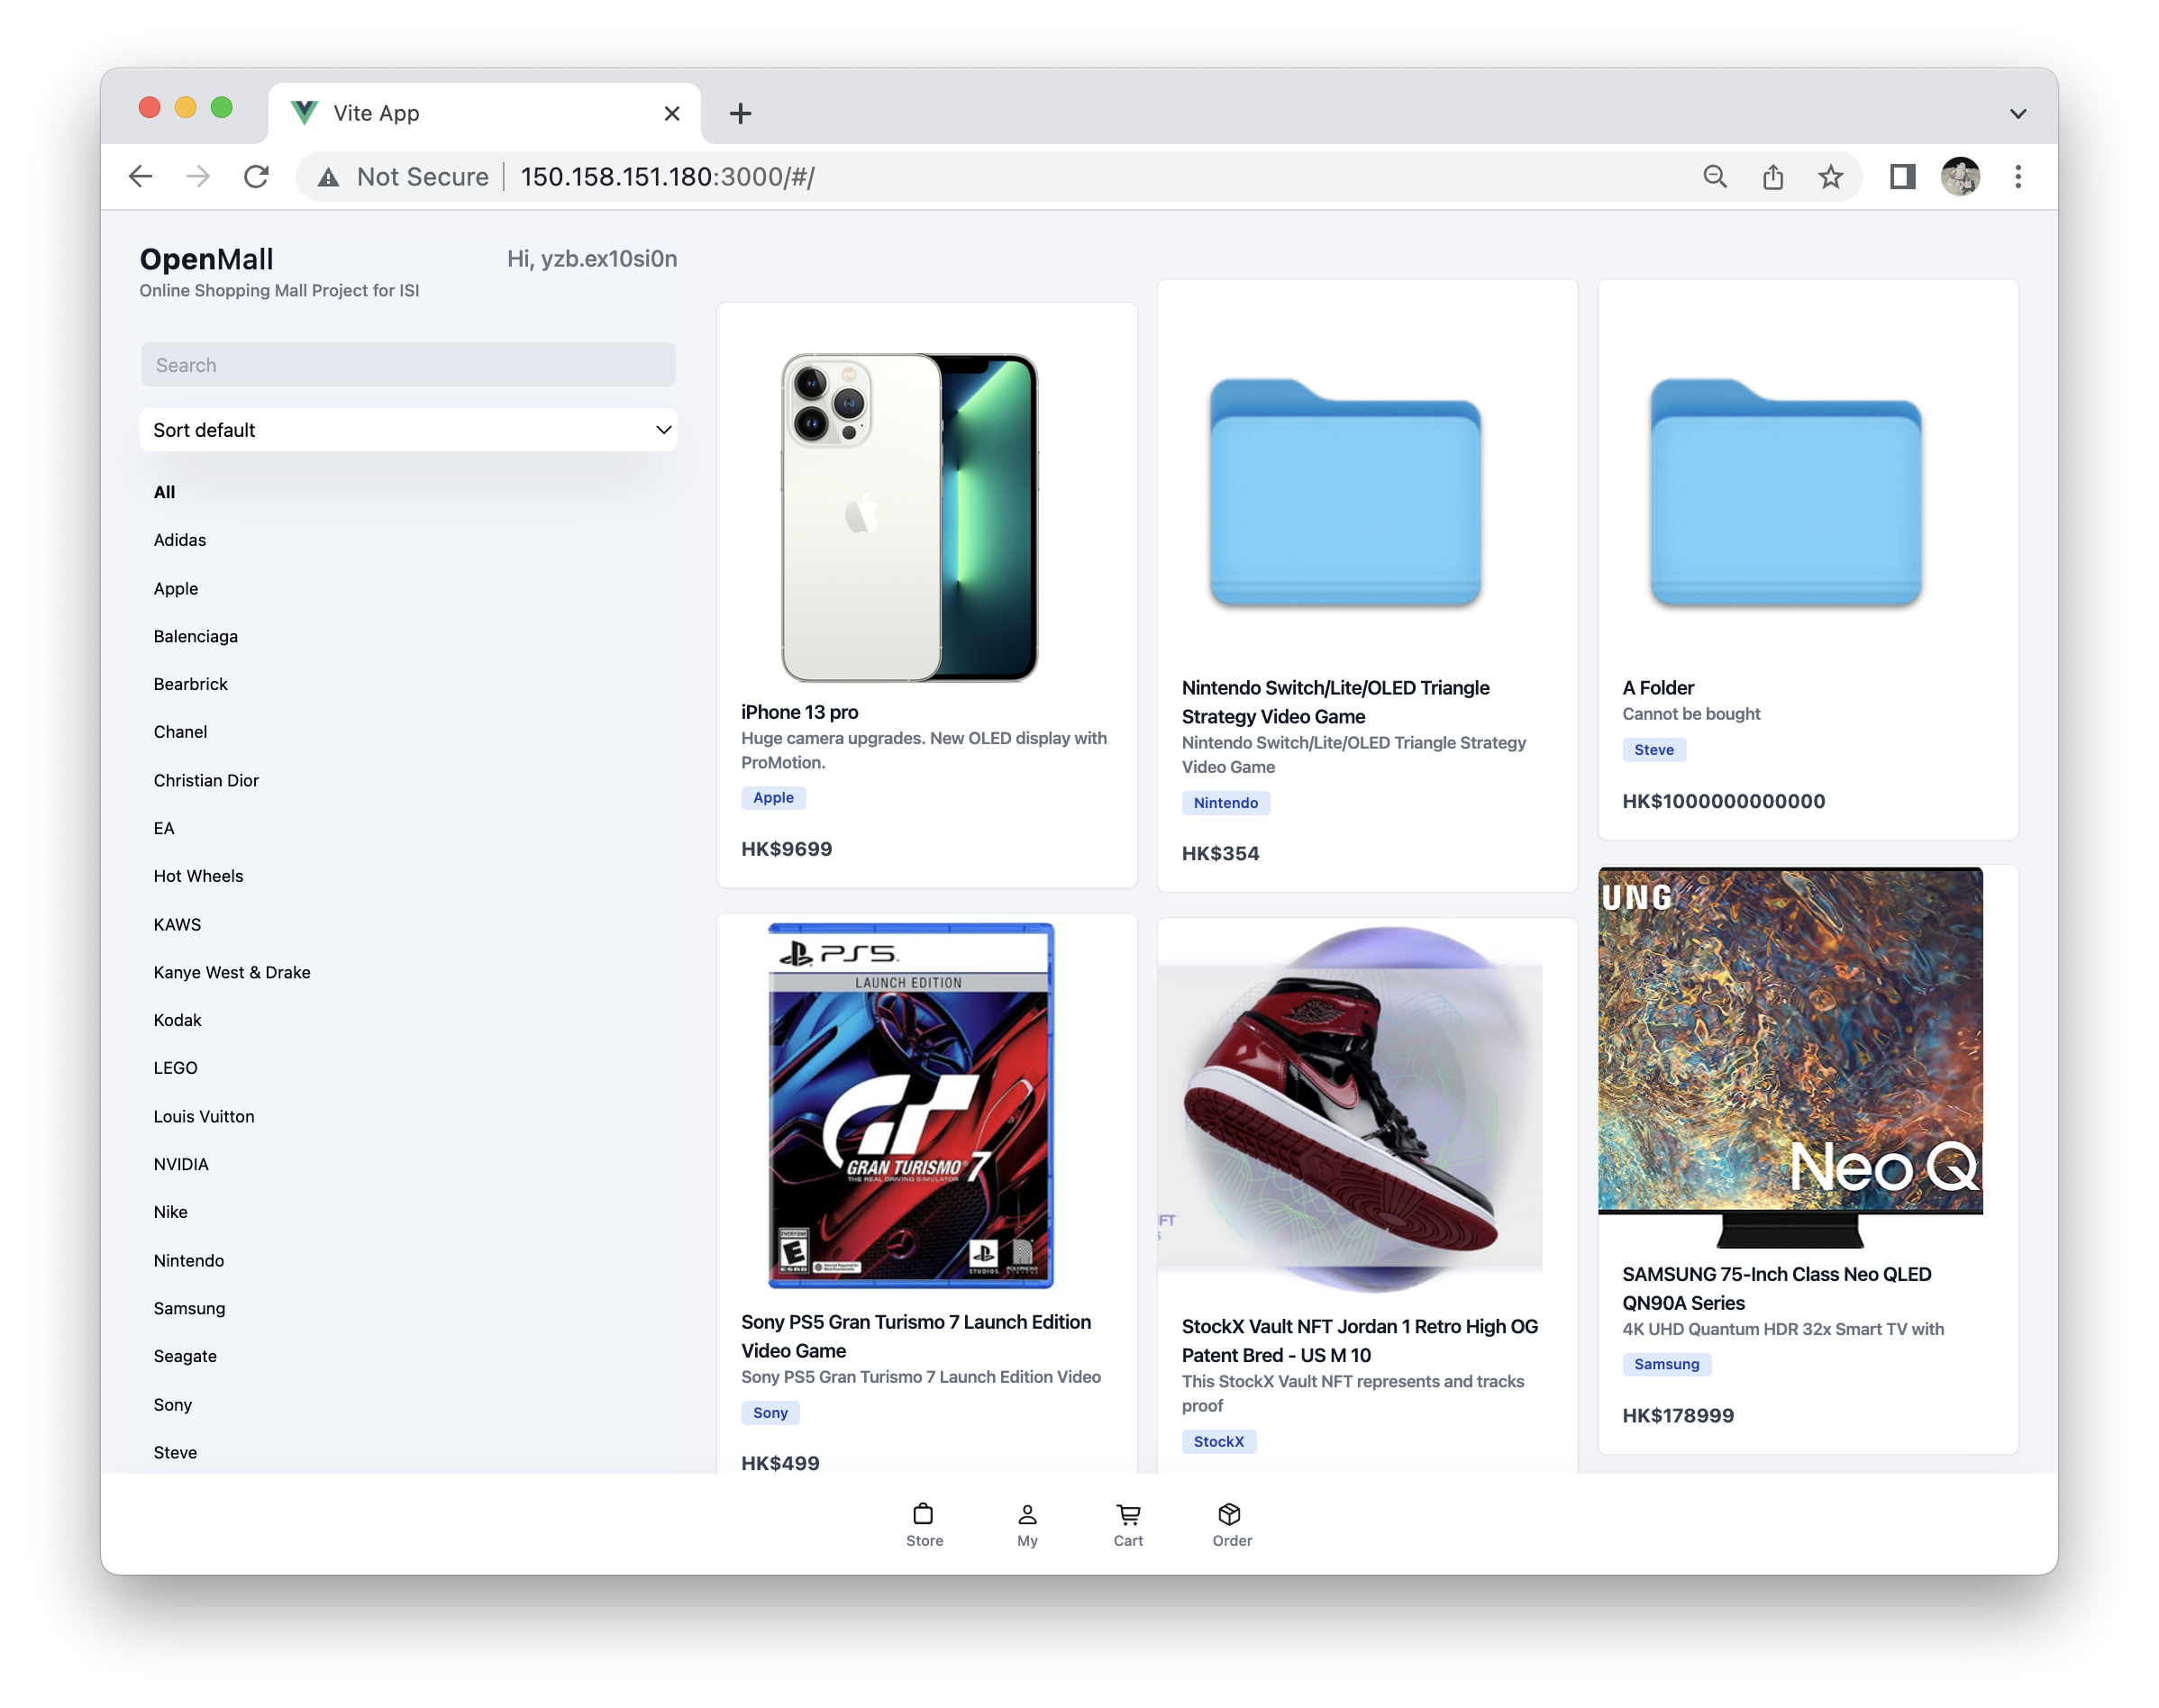
\includegraphics[width=1\textwidth]{waterfall.png}
    \caption{\label{fig:waterfall}Waterfall column of content}
\end{figure}

\leavevmode
\\\\
The original design of the item list is based on the grid view of Tailwind CSS. However, the outcome is not so pretty due to the fixed height of all item cards. Text and images are usually not within a similar box height, so the grid view generates a weird look. Hence, we change the grid layout to the waterfall column layout, as seen in listing  \ref{listing:columnLayout}. 

\begin{listing}[!htp]
\begin{minted}{html}
<div v-if="displayed_products.length >= 3" class="lg:columns-3 lg:ml-8 lg:h-full">
        ...
</div>
\end{minted}
\caption{Waterfall column layout in Desktop browser}
\label{listing:columnLayout}
\end{listing}

\leavevmode
\\\\
When a user is using OpenMall using a mobile browser or App, the waterfall column layout does not fit the small screen. The layout will automatically change to the linear listing. as shown in Figure \ref{fig:mobileLayout}.

\begin{figure}[!htp]
    \centering
    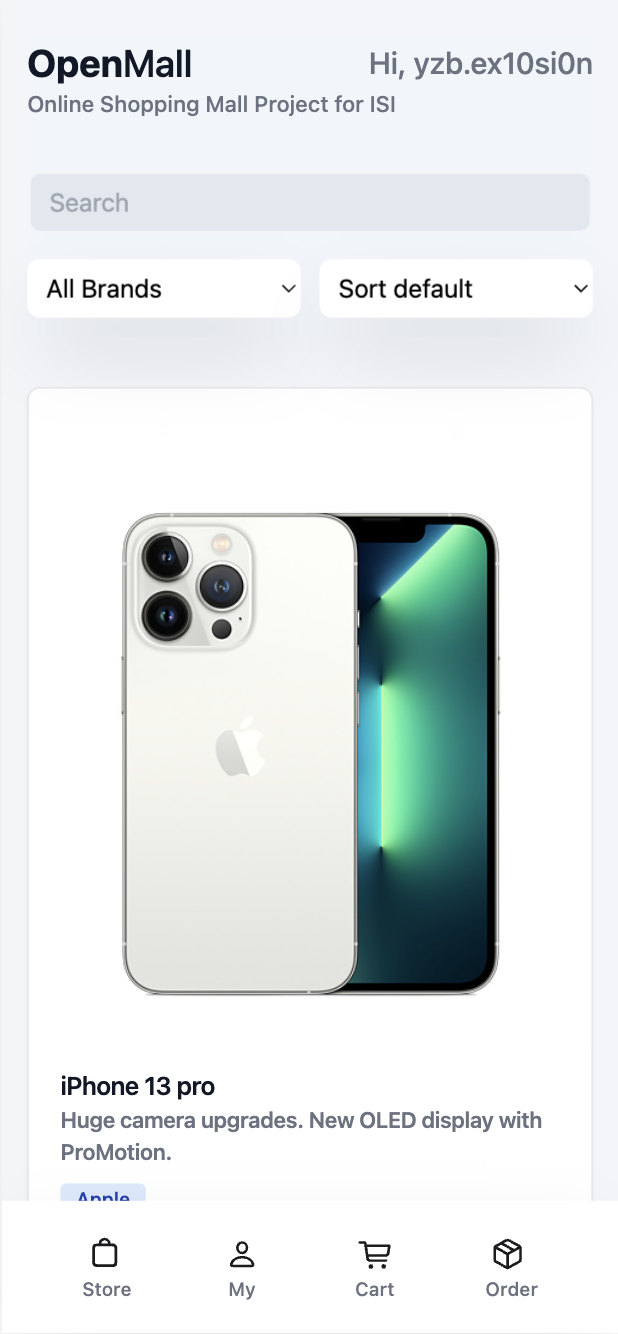
\includegraphics[width=0.3\textwidth]{mobileLayout.png}
    \caption{\label{fig:mobileLayout}Mobile linear listing layout}
\end{figure}


\subsection{Implementation of iOS App}

The implementation process of the iOS Universal App is on the development platform of macOS Xcode. SwiftUI helps the developer build great-looking apps across all Apple platforms with the power of Swift — and as little code as possible. In addition, a single project can run on both iOS, iPadOS, and even macOS with the same source code. The Xcode IDE supports many advanced features such as drag and drops to manage the structure of code snippets. It has a concise UI and powerful functionality. It also has the complete support of Vim.

\begin{figure}[!htp]
    \centering
    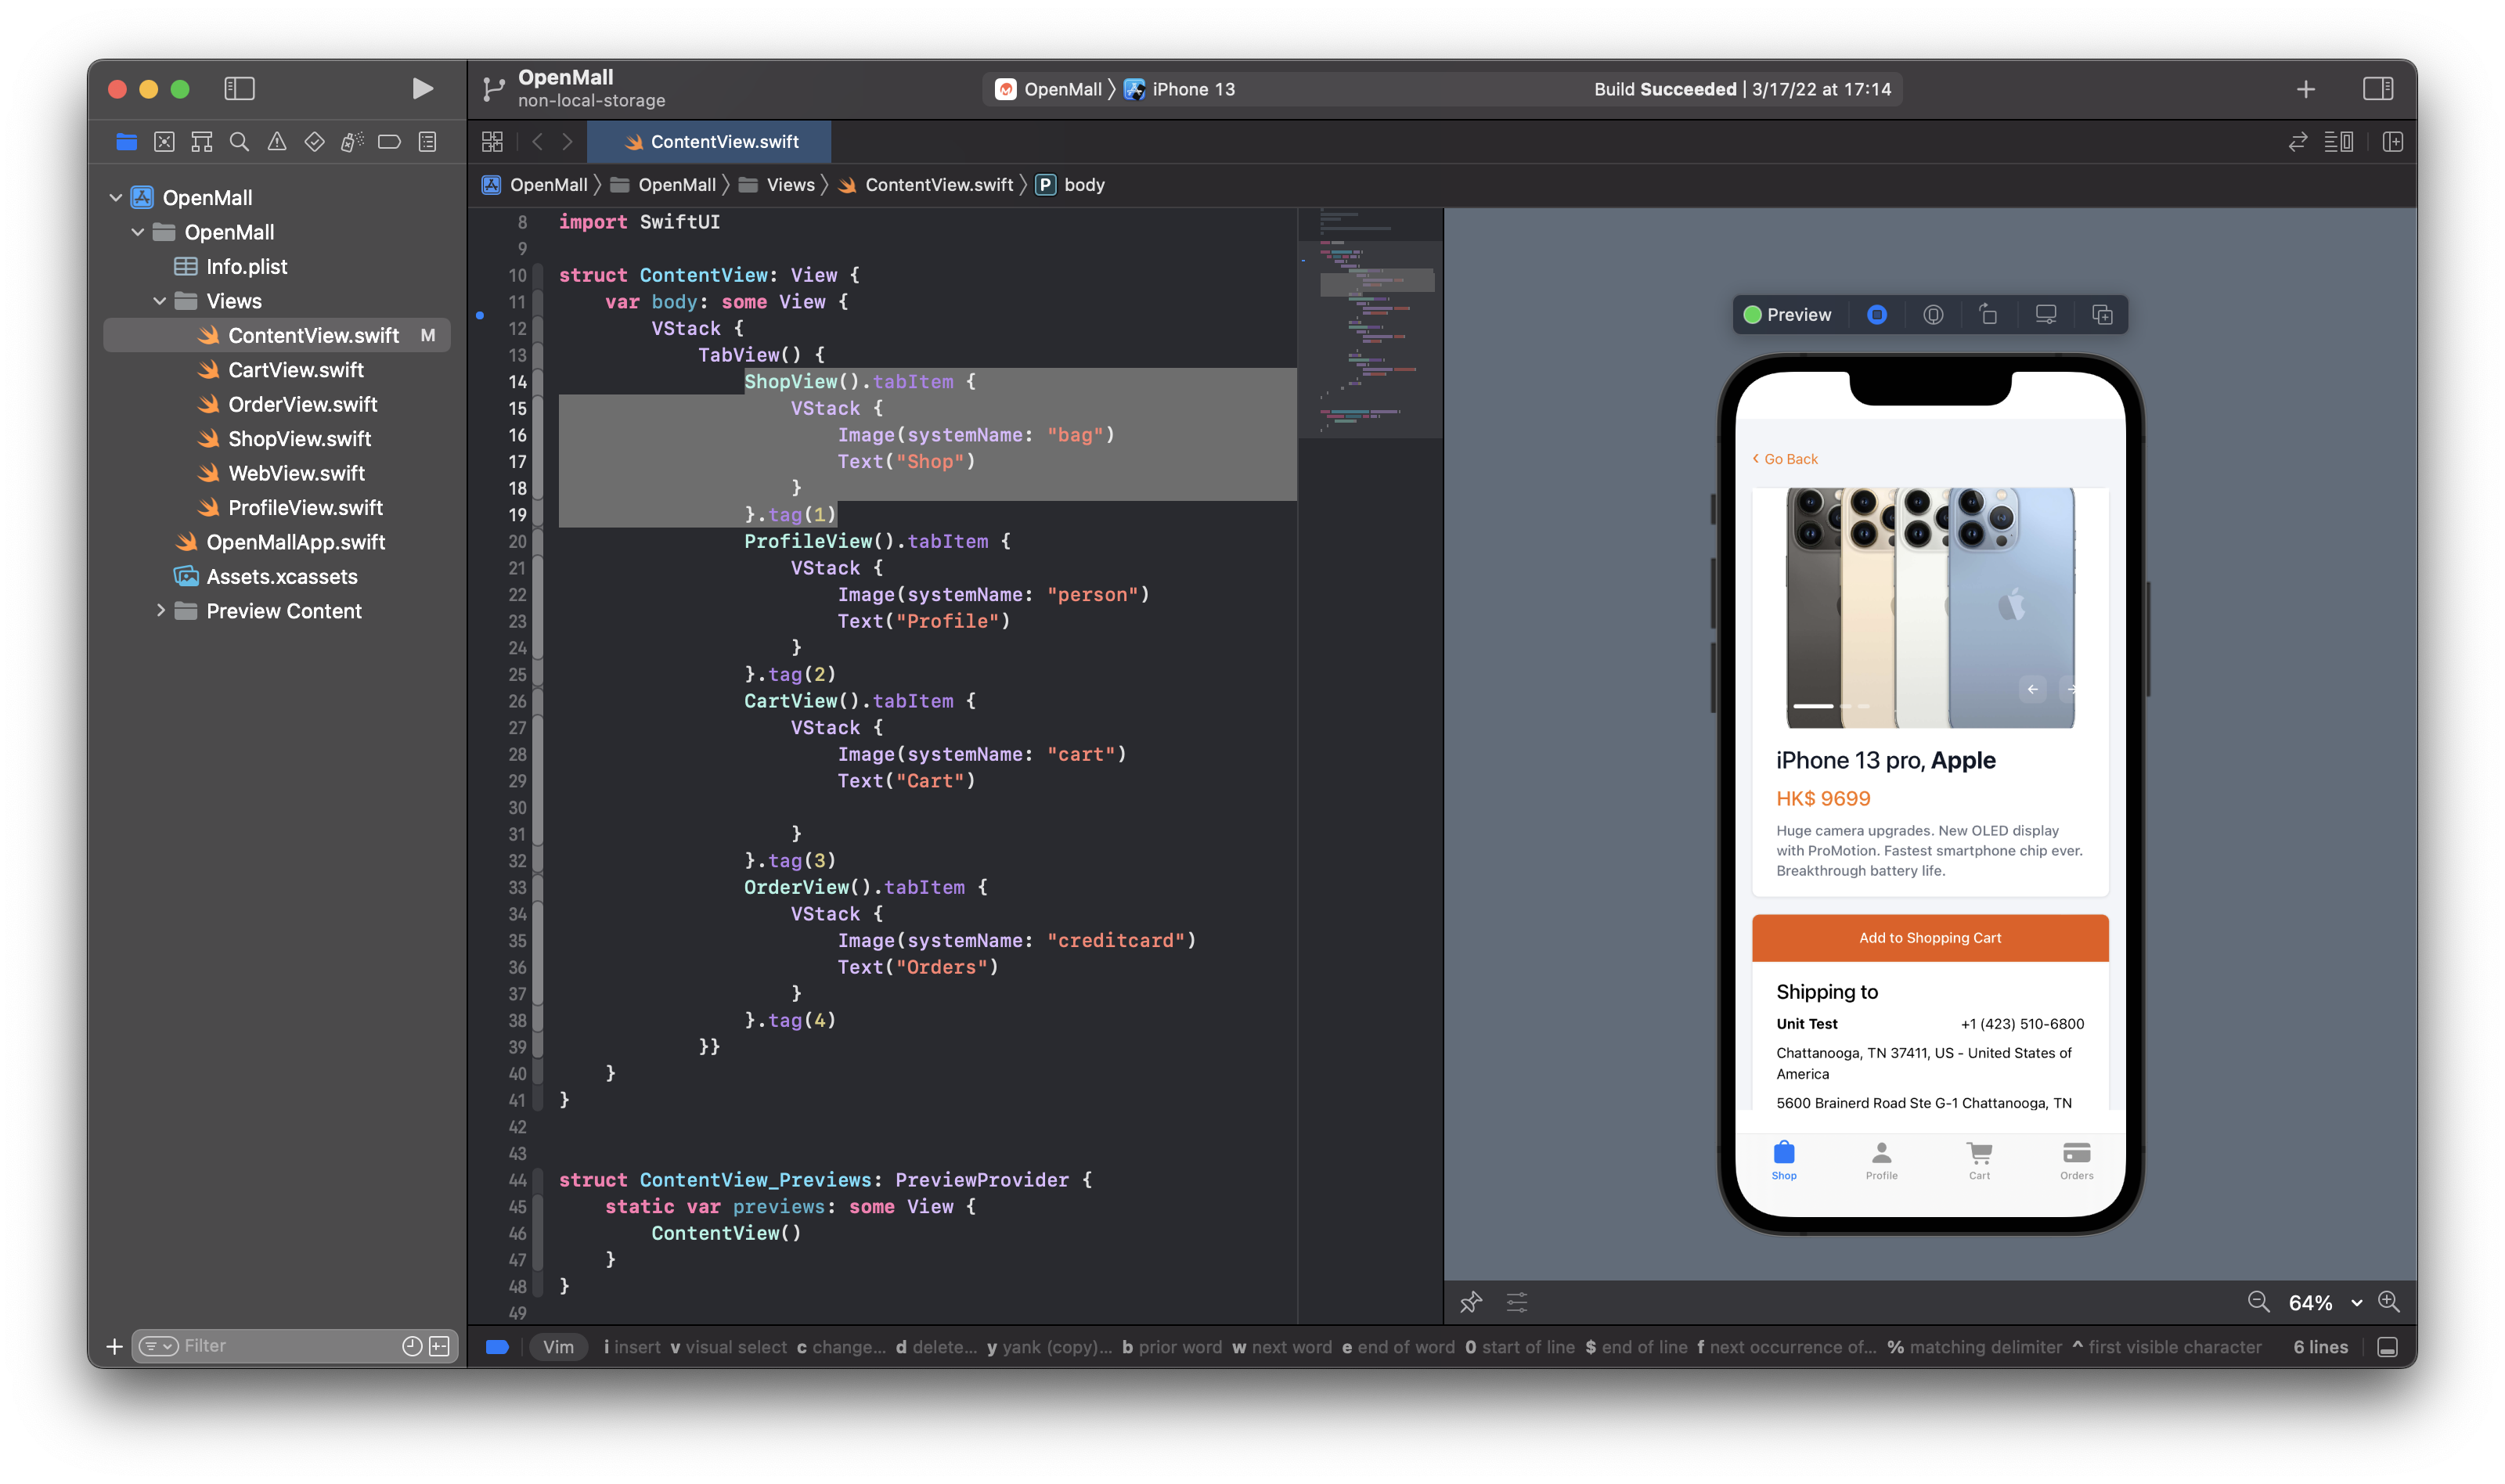
\includegraphics[width=0.9\textwidth]{xcode.png}
    \caption{\label{fig:Xcode}Xcode IDE Interface}
\end{figure}

\subsubsection{Hybrid Tab View Application}
The structure of the OpenMall iOS App is based on the template shown in Figure \ref{fig:tabview} of the SwiftUI App. The OpenMall is a tab view App. It has tabs for different functionalities underneath the screen. The Swift code to implement the tab-base architecture is shown in Listing \ref{listing:tabview}.

\begin{listing}[!htp]
\begin{minted}{swift}
import SwiftUI

struct ContentView: View {
    var body: some View {
        VStack {
            TabView() {
                ShopView().tabItem {
                    VStack {
                        Image(systemName: "bag")
                        Text("Shop")
                    }
                }.tag(1)
                // more tabs omitted
            }
        }
    }
}
\end{minted}
\caption{Implement Tab views in Swift}
\label{listing:tabview}
\end{listing}

\begin{figure}[!htp]
    \centering
    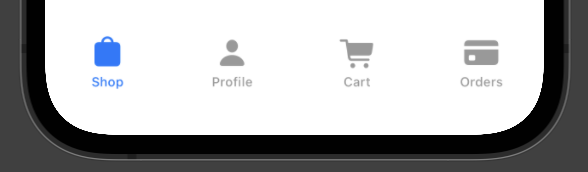
\includegraphics[width=0.4\textwidth]{tab.png}
    \caption{\label{fig:tabview}Tab View}
\end{figure}

\leavevmode
\\\\
Hybrid apps work similar to Web apps but, like native apps, are downloaded to the device. Like Web apps, hybrid apps are typically implemented by a front-end technical stack. Hybrid apps run code inside a container. The device's browser engine is used to render HTML and JavaScript and native APIs to access device-specific hardware. Although a hybrid app will typically share similar navigation elements as a Web app, whether or not the application can work offline depends on its functionalities. If an application does not need support from a database, it can function offline. Since we have implemented the complex functions and UI by the front-end technical stack of Vue.js 3.0 and Tailwind CSS. To simplify the development process of the mobile app,  we adopted view-based WebKit web view components to implement each tab page of functionalities. That meets the philosophy of a hybrid web app. 


\subsubsection{Project Structure}

For the SwiftUI project under Xcode 13.0, the project structure recommended by Apple is a hierarchy view. Four major pages of OpenMall are the Item list, User profile, Shopping cart, and Orders. The corresponding SwiftUI views are \verb|ShopView|, \verb|ProfileView|, \verb|CartView|, and \verb|OrderView|. In addition, the \verb|WebView| is the helper view class implemented the WebKit web view interface (as shown in listing \ref{webview}). All of the views are called inside \verb|ContentView|.

\begin{listing}[!htp]
\begin{minted}{swift}
import WebKit

struct WebView: UIViewRepresentable {
    var url: URL
    
    func makeUIView(context: Context) -> WKWebView {
        return WKWebView()
    }
    
    func updateUIView(_ uiView: WKWebView, context: Context) {
        let request = URLRequest(url: url)
        uiView.load(request)
    }
}
\end{minted}
\caption{Implementation of WebView in Swift}
\label{webview}
\end{listing}

\leavevmode
\\\\
For the four major views in the last paragraph, the code implementation is similar. As an example of \verb|ShopView.swift| . For the item list, the code is shown at \ref{listing:shopview}.

\begin{listing}[!htp]
\begin{minted}{swift}
import SwiftUI

struct ShopView: View {
    var body: some View {
        let urlString: String = baseURL + "#/"
        VStack {
            WebView(url: URL(string: urlString)!)
                .cornerRadius(0)
                .navigationBarTitleDisplayMode(.inline)
                .ignoresSafeArea(.all, edges: .top)
        }
    }
}

struct ShopView_Previews: PreviewProvider {
    static var previews: some View {
        ShopView()
    }
}
\end{minted}
\caption{Implementation of ShopView in Swift}
\label{listing:shopview}
\end{listing}

\begin{figure}[!htp]
    \centering
    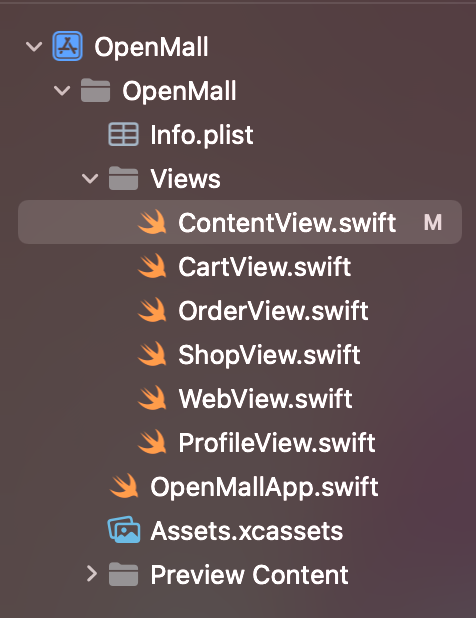
\includegraphics[width=0.4\textwidth]{file-struct.png}
    \caption{\label{fig:Xcode}Xcode Project Structure}
\end{figure}

\leavevmode
\\\\
Due to the intention of security protection, Apple canceled to support web view via the HTTP protocol in Xcode. However, registering an HTTPS certification costs a high price. In addition, we have not specified a domain name for OpenMall. It is needed to change the project configuration file \verb|info.plist| by adding lines of code to allow all of the unsecured connections.

\begin{listing}[!htp]
\begin{minted}{xml}
<key>NSAppTransportSecurity</key>
<dict>
  <!--Include to allow all connections (DANGER)-->
  <key>NSAllowsArbitraryLoads</key>
      <true/>
</dict>
\end{minted}
\caption{Enable Unsecured connections via HTTP}
\label{infoplist}
\end{listing}
\leavevmode
\\\\
After implementing all of the essential tab views, Xcode can build OpenMall for the simulator and iPhone. After validating the Apple developer certificate. The app can be distributed as a pre-released edition to mobile devices with the developer profile on OpenMall. Furthermore, to distribute the release version. We need to pay for the Apple developer license. Then the OpenMall can be downloaded from the App Store.

\begin{figure}[!htp]
    \centering
    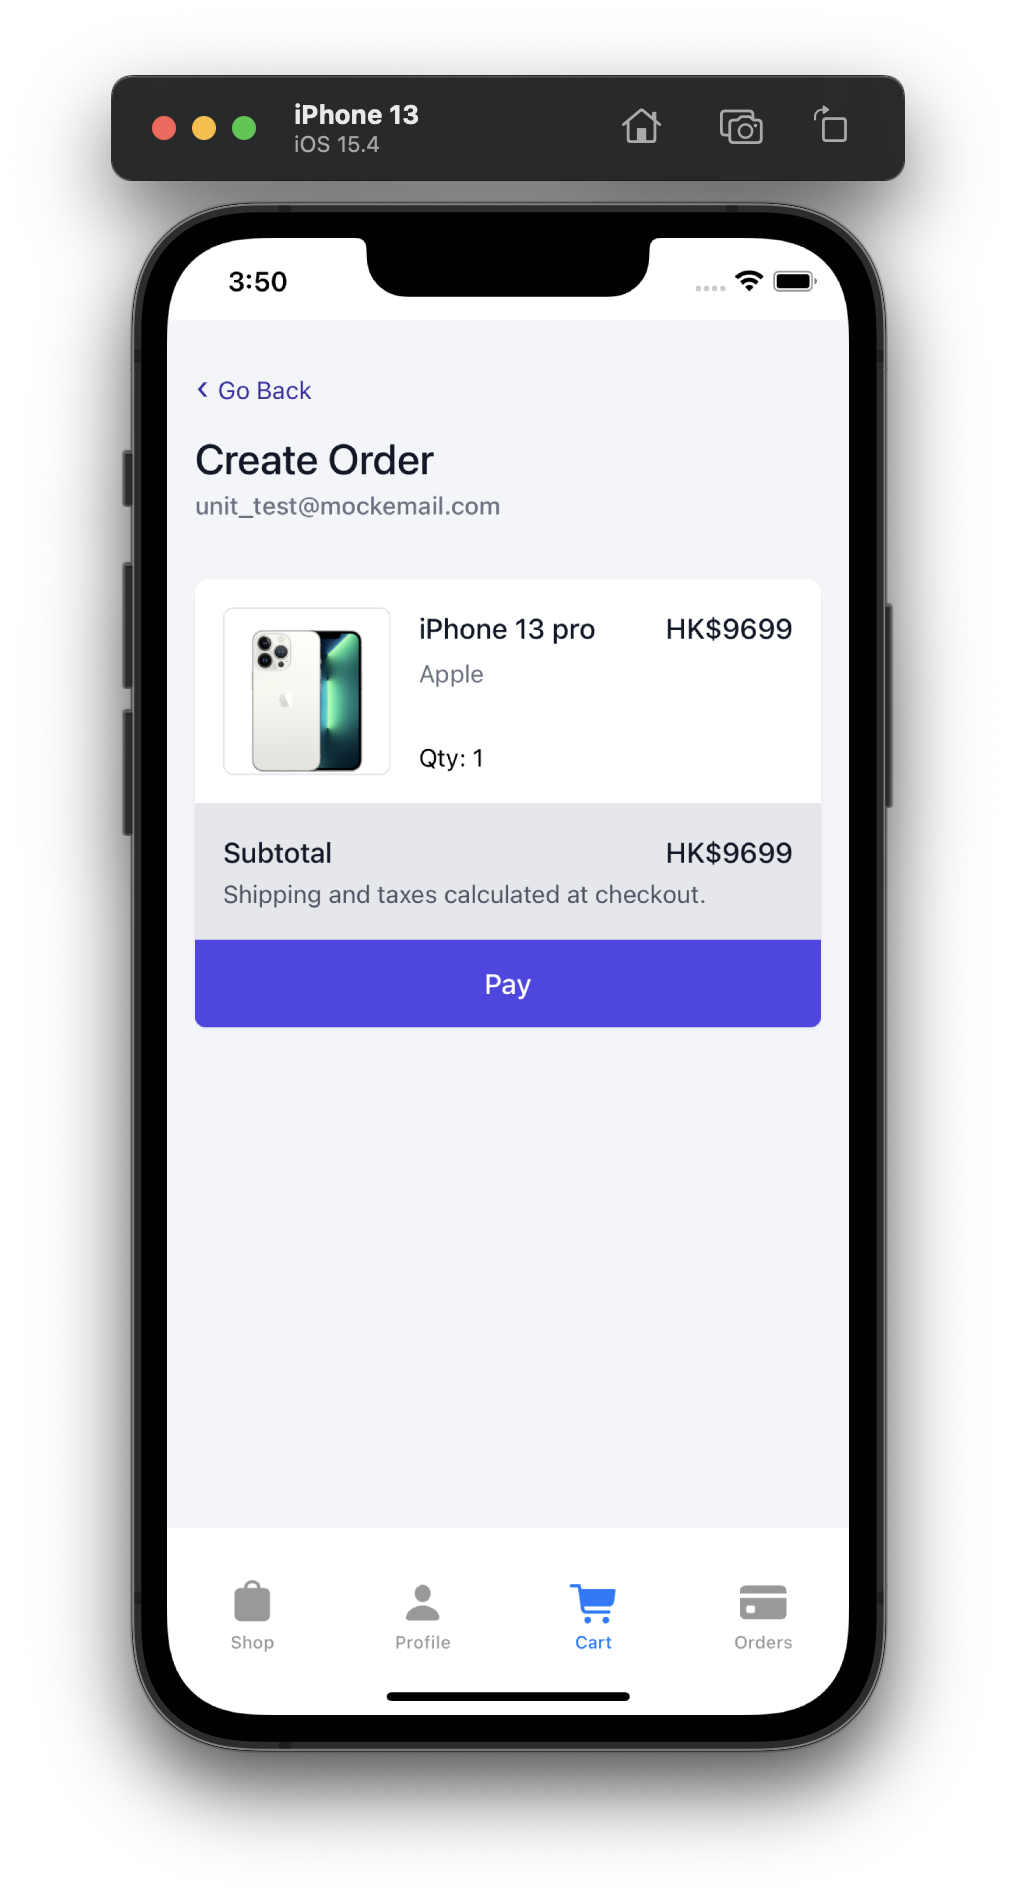
\includegraphics[width=0.35\textwidth]{simulator.png}
    \caption{\label{fig:Xcode}OpenMall running on iPhone 13 simulator}
\end{figure}
\clearpage
\subsection{Persist User Status in separation of front-end and back-end}

As we know, the HTTP protocol is stateless, which means that if we have authenticated a user, the next time he/she makes a request, the server does not be able to know who he/she is, and he/she have to authenticate again. Therefore, user status persistence is indispensable. In the traditional way, the data of the user who has been authenticated is stored on the server, such as Session. User requests with the session ID, and Websites use the session ID to respond to user interactions during a web session.\cite{sec} But it comes with an irremediable shortage which is the server has to create a record to store an authenticated user, and with the number of users increasing the load of the server is increasing soon. 
\\\\
To reduce the load of the server and persist user status, JSON Web Token is used in OpenMall project. JSON Web Token (JWT) is an open standard (RFC 7519) that defines a compact and self-contained way for securely transmitting information between parties as a JSON object. This information can be verified and trusted because it is digitally signed.\cite{jwt} Both JSON Web Token and Session are used to store user data, but JSON Web Token decentralizes user data to the client-side. JSON Web Token is stateless, no user information is stored in the server or session. Hence, procedures of interaction between the front-end and the back-end are as followed figure\ref{fig:JWT}.

\begin{figure}[!htp]
    \centering
    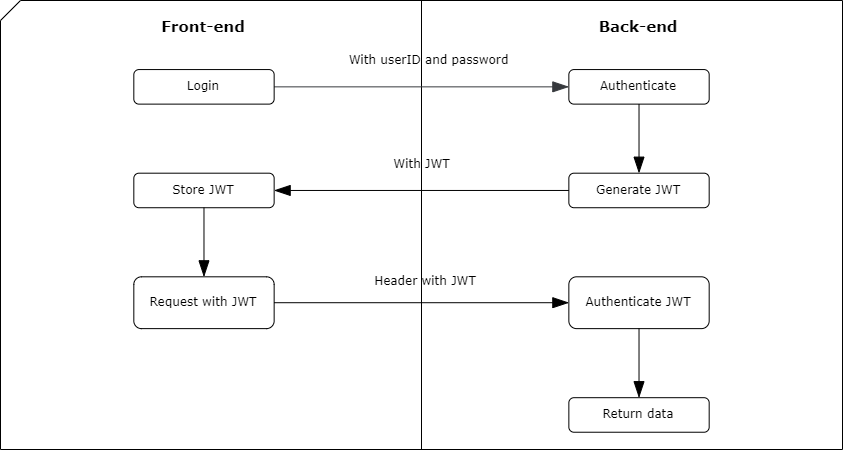
\includegraphics[width=0.9\textwidth]{JWT.png}
    \caption{\label{fig:JWT}Interaction between front-end and back-end with JWT}
\end{figure}

\subsubsection{Generation of JSON Web Token}

We have to have a primary JWT if we are going to use it as users’ credentials. Then, add an expiration for this token. Finally, the user will have to sign in again to get a new token when his/her token is expired.  
\\\\
In the OpenMall project, we installed \verb|python-jose| to generate and verify the JWT token in Python. We randomly generated an initial JWT token and assigned it to \verb|SECRET _KEY|. We created variables for the algorithm used to sign the JWT token and the expiration of the token. Besides, the function of creating a new JWT token for users is created. The python code is shown below in Listing 37.

\begin{listing}[!htp]
\begin{minted}{python}
from jose import JWTError, jwt

SECRET_KEY = "6a5c696a4469597fe2962bcd83e05846fe86ec5bbde835c7983955a295e092da"
ALGORITHM = "HS256"
ACCESS_TOKEN_EXPIRE_MINUTES = 4320

class Token(BaseModel):
    access_token: str
    token_type: str = Field(default='Bearer')
	
def create_access_token(data: dict, expires_delta: Optional[timedelta] = None):
    to_encode = data.copy()
    if expires_delta:
        expire = datetime.utcnow() + expires_delta
    else:
        expire = datetime.utcnow() + timedelta(minutes=10080)
    to_encode.update({"exp": expire})
    encoded_jwt = jwt.encode(to_encode, SECRET_KEY, algorithm=ALGORITHM)
    return encoded_jwt

\end{minted}
\caption{Generation of JSON Web Token}
\label{JWT grneration}
\end{listing}

\subsubsection{Front-end requests and stores JSON Web Token}

Moving to the front end, it should be able to access the JWT token from the back-end and store the JWT token in the local storage. Moreover, add JWT token to the Authentication part of HTTP headers on each request.
\\\\
In the OpenMall project, the front-end uses Axios to request the API for accessing JWT token after the user login in successfully. The Axios request is attached in Listing 38.

\begin{listing}[!htp]
\begin{minted}{javascript}
const queryToken = "http://" + config.apiServer + ":" + config.port + "/api/token/"
axios.post(queryToken, qs.stringify({
  username: email.value,
  password: password.value
})).then((res) => {
  store.commit('chgLogin', {
    Authorization: res.data.access_token
  });
  localStorage.setItem('Authorization', res.data.access_token);
})
\end{minted}
\caption{Axios request for JWT token}
\label{Axios for JWT}
\end{listing}
\leavevmode
\\\\
Then, we store it in the local storage of the client-side. The corresponding code is as below.

\clearpage

\begin{listing}[!htp]
\begin{minted}{javascript}
chgLogin(state, authorization) {
  state.Authorization = authorization;
  localStorage.setItem('Authorization', authorization);
}
\end{minted}
\caption{Store JWT token}
%\label{listing:6}
\end{listing}
\leavevmode
\\\\
If we have JWT token in the local storage of client-side, we will be able to get it and add it to the Authentication part of each HTTP request.

\begin{listing}[!htp]
\begin{minted}{javascript}
axios.defaults.headers.common['Authorization'] = "Bearer " +
localStorage.getItem('Authorization');

axios.interceptors.request.use(
  config => {
    if (config.headers === undefined) {
      config.headers = {};
    }
    if (localStorage.getItem('Authorization')) {
      config.headers.Authorization = "Bearer " + localStorage.getItem('Authorization');
    }

    return config;
  },
  error => {
    return Promise.reject(error);
  });
\end{minted}
\caption{Add JWT token to each request}
\label{Add JWT}
\end{listing}

\subsubsection{JSON Web Token verification and data return APIs}

Finally, with the requests from the front-end, the back-end API needs to verify the token. After that, find the user information by interacting with the database and return it.
\\\\
For the OpenMall project, the asynchronous function named \verb|get_current_user| was created to verify the token and get the user information. In the function, the token will decode by a method included in Python \verb|jwt| library and return the user information after successfully verifying, otherwise it will raise a \verb|TokenVerifyException| error. Meanwhile, the API for getting current user information was created.The python code is as follow.

\begin{listing}[!htp]
\begin{minted}{python}
async def get_current_user(token: str = Depends(oauth2_scheme)):
    TokenVerifyException = HTTPException(
        status_code= 401,
        detail="Could not validate credentials",
        headers={"WWW-Authenticate": "Bearer"},
    )
    try:
        payload = jwt.decode(token, SECRET_KEY, algorithms=[ALGORITHM])
        username: str = payload.get("sub")
        if username is None:
            raise TokenVerifyException
        token_data = TokenData(username=username)
    except PyJWTError:
        raise TokenVerifyException
    from db.database import get_user
    user = get_user(email=token_data.username)
    if user is None:
        raise TokenVerifyException
    return user
	
@app.post('/api/token/')
async def login_for_access_token(form_data: OAuth2PasswordRequestForm=Depends()):
    from db.database import login_check
    user = login_check(form_data.username, form_data.password)
    if user['status'] == 'success':
        access_token_expire = timedelta(minutes=ACCESS_TOKEN_EXPIRE_MINUTES)
        access_token = create_access_token(data={"sub": form_data.username},
            expires_delta=access_token_expire)
    else:
        raise HTTPException(
        status_code= 401,
        detail="Could not validate credentials",
        headers={"WWW-Authenticate": "Bearer"},
    )
    return {"access_token": access_token, "token_type": "bearer"}

\end{minted}
\caption{JSON Web Token verification and data return APIs}
\label{JWT verification and data return}
\end{listing}

\clearpage

\section{Result and Discussion}

\subsection{Project Outcome}

\subsubsection{Customer-Product list with paging, search and filter}
The user opens the Open Mall and sees a list of products. Each product will display some basic information in the form of a card view [Figure \ref{fig:card view}], including product name, brand, price, and a thumbnail image. And each product has a tag of the brand it belongs to[Figure \ref{fig:product list}].

\begin{figure}[!htp]
    \centering
    
\includegraphics[width=0.3\textwidth]{card view 2.png}
    \caption{\label{fig:card view}Card view}
\end{figure}

\begin{figure}[!htp]
    \centering
    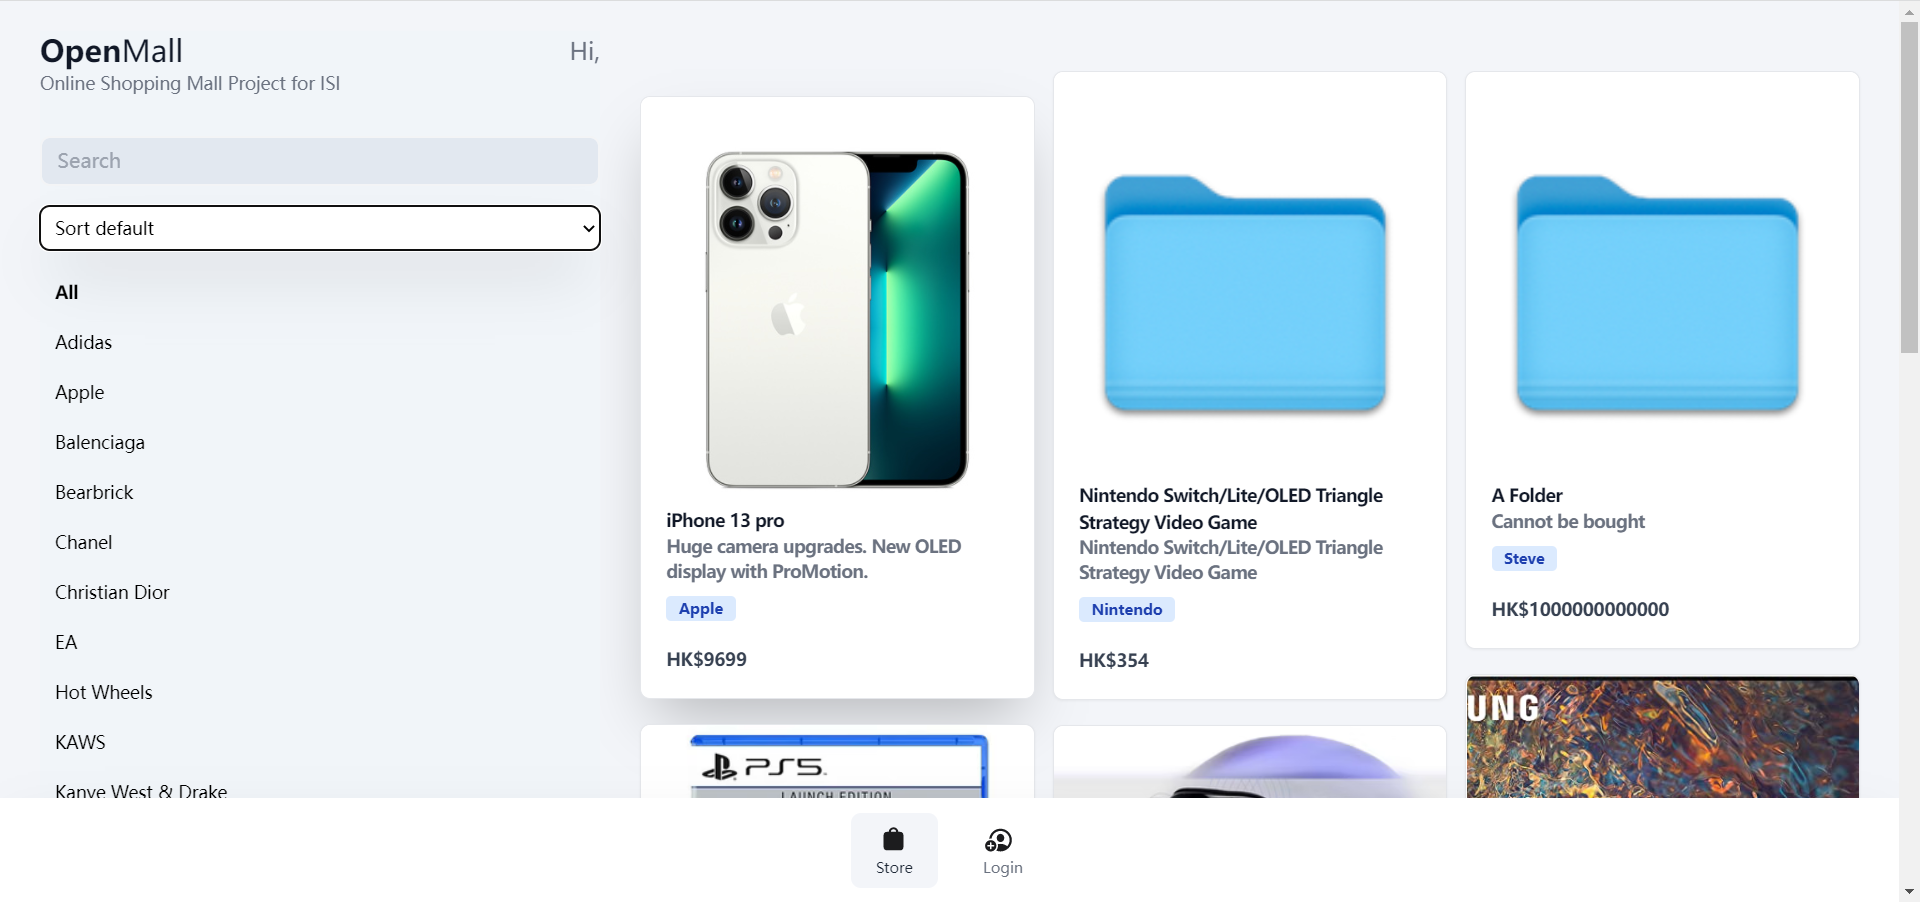
\includegraphics[width=0.8\textwidth]{product list.png}
    \caption{\label{fig:product list}Main interface for the Customer}
\end{figure}

To control the number of items displayed on each page to provide a better user experience, paging is set at the bottom right corner of the page.[Figure \ref{fig:paging}]  Users can skip to the previous or next page by clicking “Next” or “Previous”. To jump directly to a specific page number,customers can enter the corresponding page number. If the entered page number is greater than the total number of pages, the system will jump to the last page. Similarly, if the number of pages entered is less than 1, it will jump to the first page.
\begin{figure}[!htp]
    \centering
    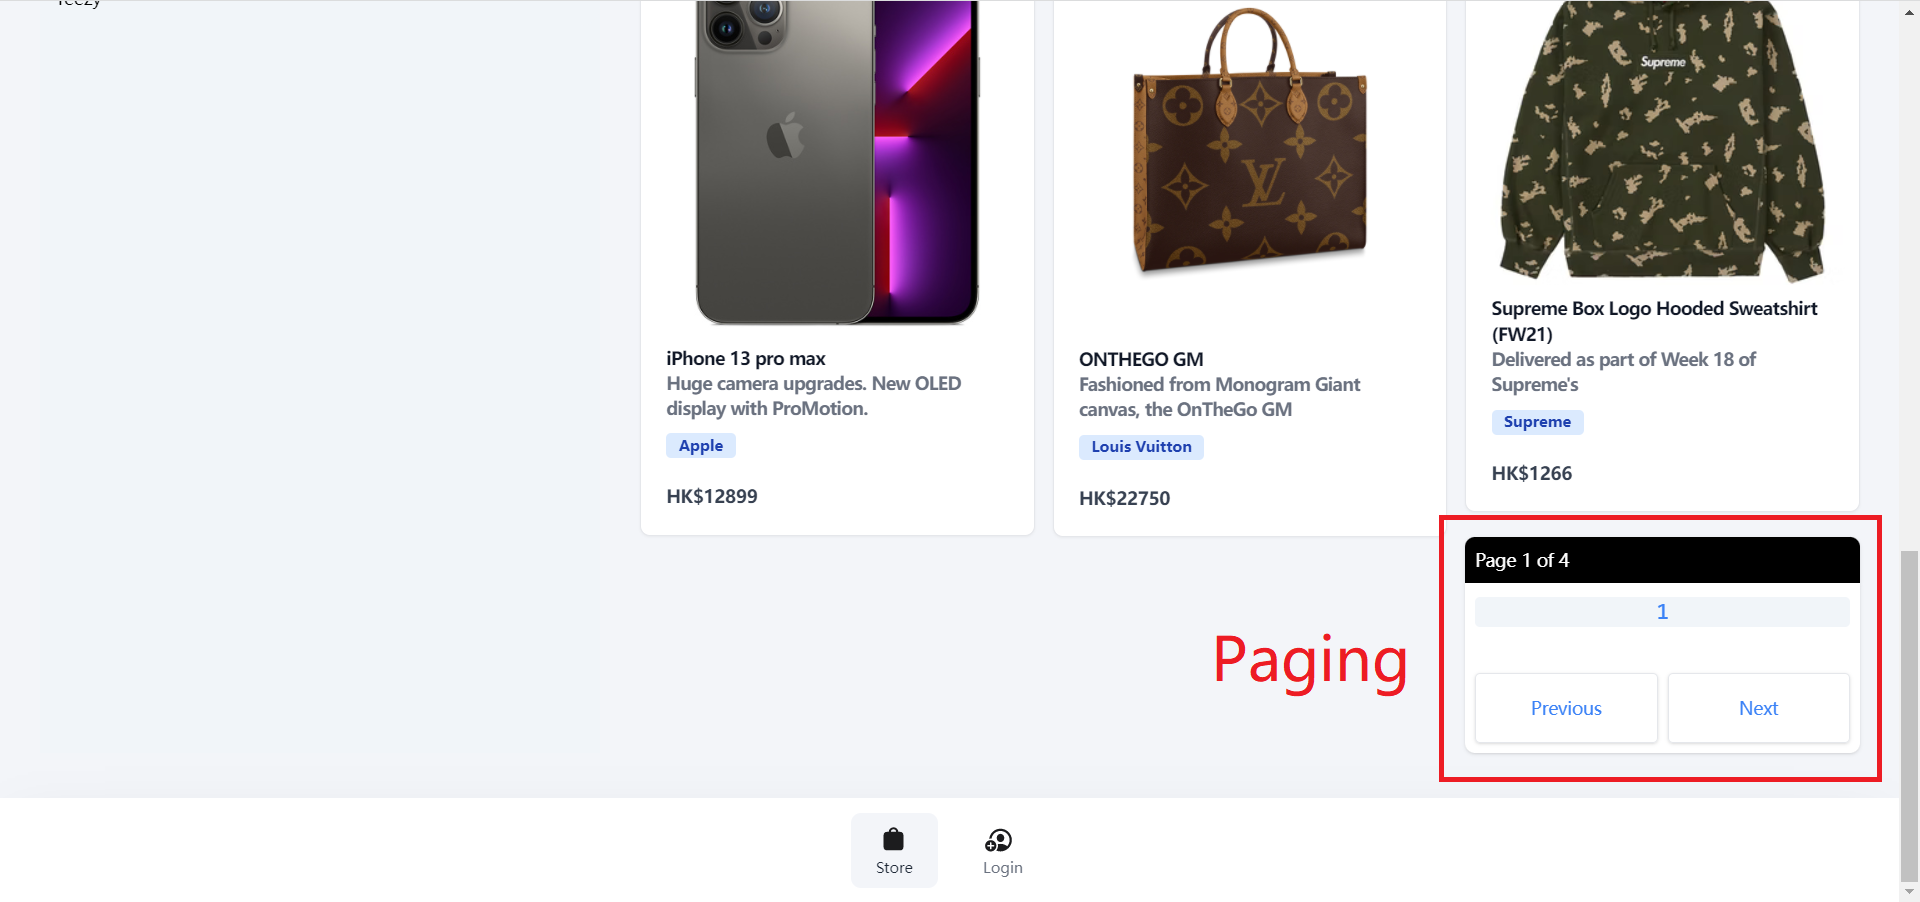
\includegraphics[width=0.6\textwidth]{paging.png}
    \caption{\label{fig:paging}Paging}
\end{figure}
\\\\
When users do not want to search for products through browse Product List, they can use a filter to select the desired brand, and then browse the filtered product list. Or, they can directly enter the keyword in the search bar to search for the product they want. "Sort by Price", from high to low or from low to high. All of these selecting tools are on the left-hand side of the website [see Figure \ref{fig:filter and search bar and sort}].
\begin{figure}[!htp]
    \centering
    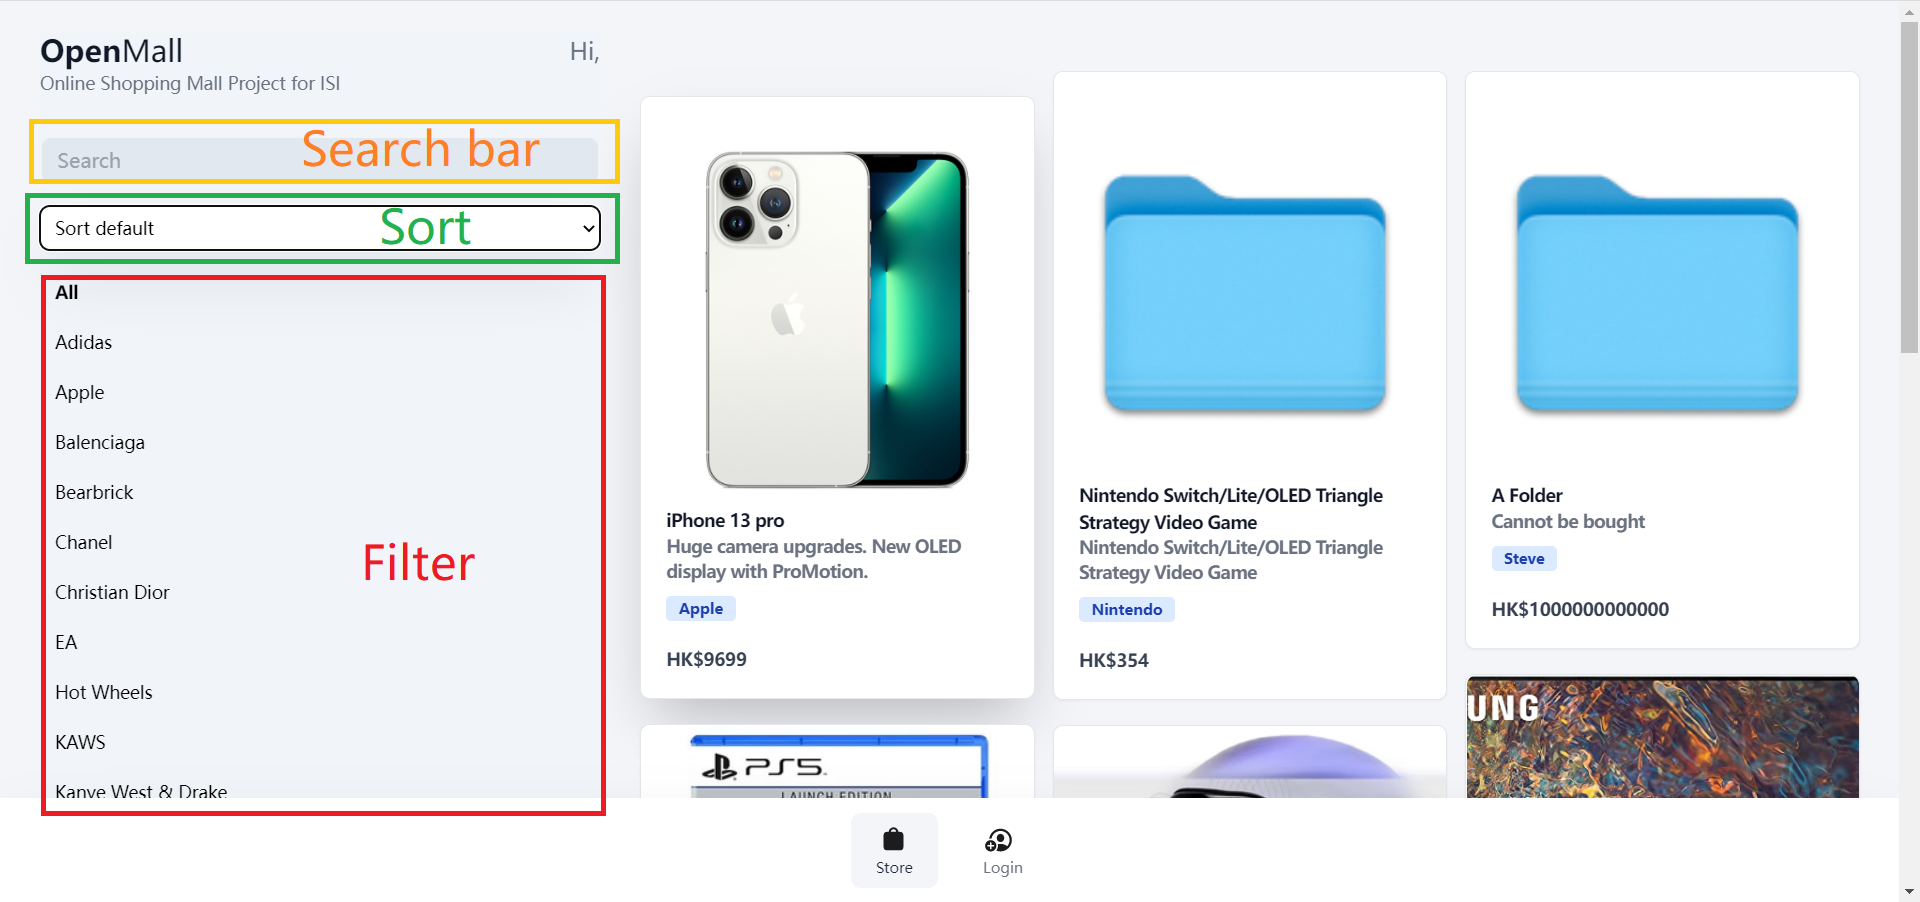
\includegraphics[width=0.6\textwidth]{search bar and sort.png}
    \caption{\label{fig:filter and search bar and sort} Filter, search bar and sort tool}
\end{figure}

\subsubsection{Customer-Product detail page}
After finding the product, customer can go to the Product Detail page by clicking on the picture of the product. On this page [see Figure \ref{fig:product detail page}], more detailed information which includes the product name, brand, price, and a thumbnail image will be shown. In addition, the product detail page also shows a detailed description as a list of at least two properties. Moreover, not only the thumbnail image, more detailed photographs will be displayed on this page. Users can press the buttons to control to displaying which photograph.
\begin{figure}[!htp]
    \centering
    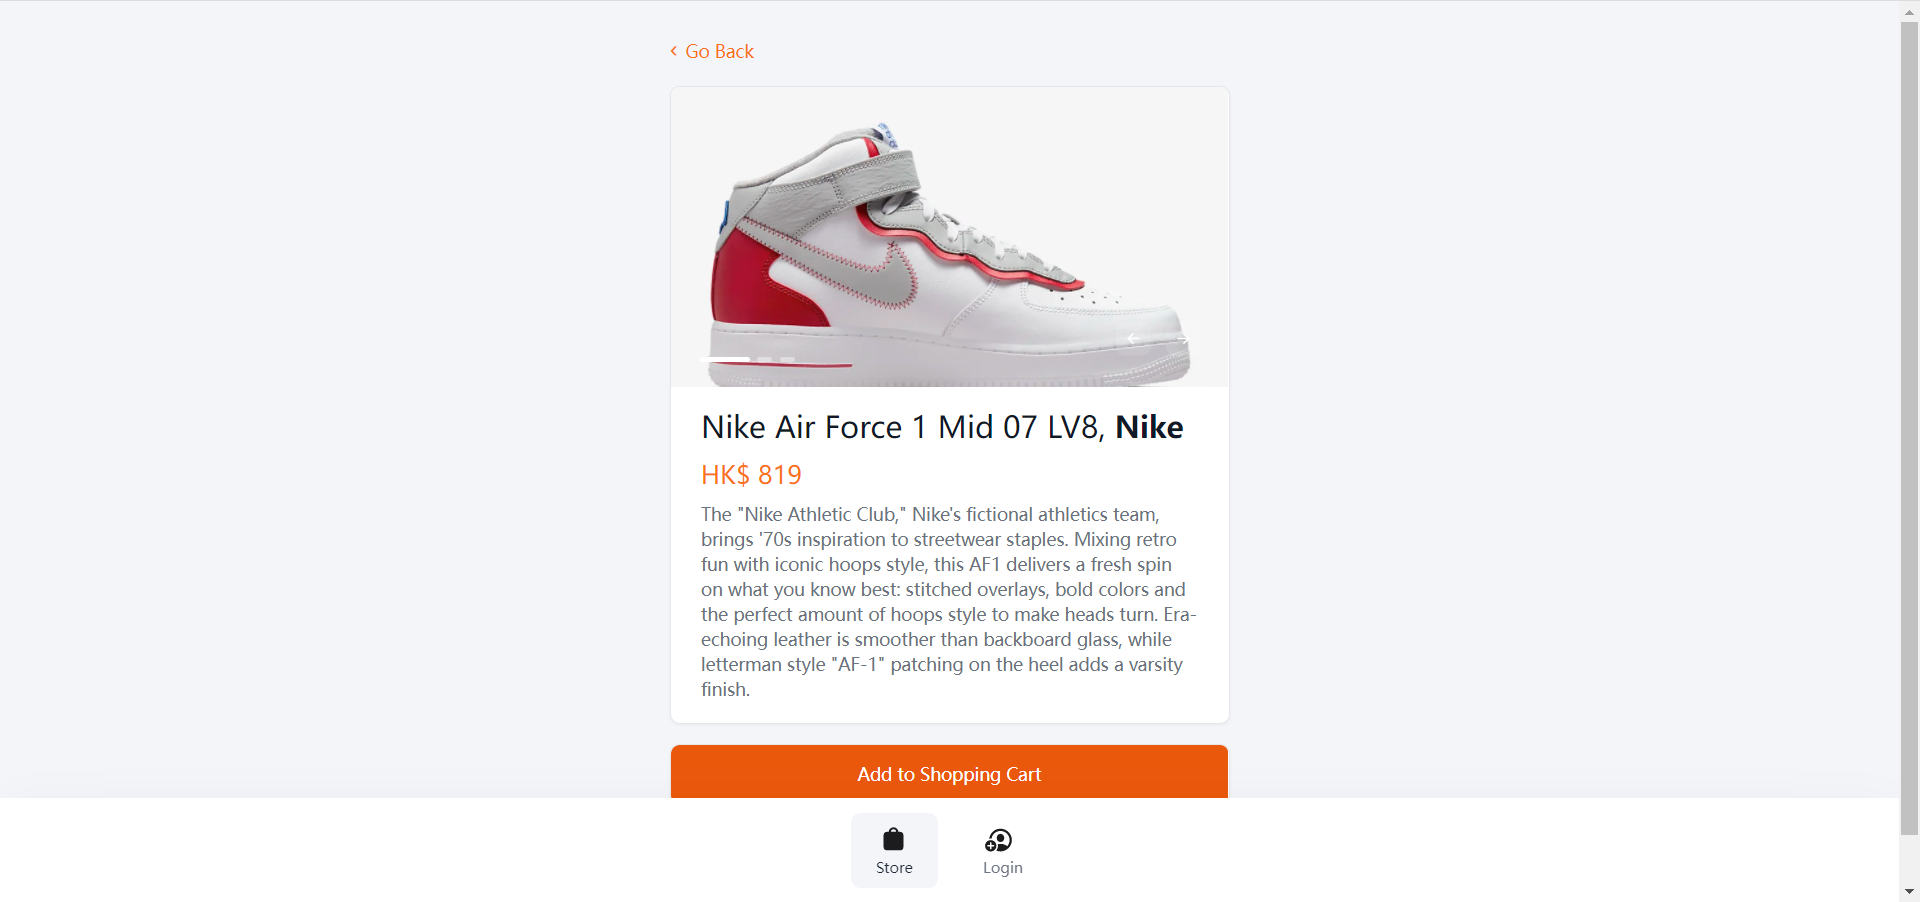
\includegraphics[width=0.6\textwidth]{product detail page.png}
    \caption{\label{fig:product detail page}Product detail page }
\end{figure}
\\\\
There is an orange button on the bottom of the product -- “Add to the shopping cart”. Users can press this bottom to add the product to the shopping cart. But there are two situations there, one is if the user is login, the product will be added to the shopping cart successfully. The content of the orange button will change to “In Shopping Cart” [see Figure \ref{fig:add in shopping_cart}].
\begin{figure}[!htp]
    \centering
    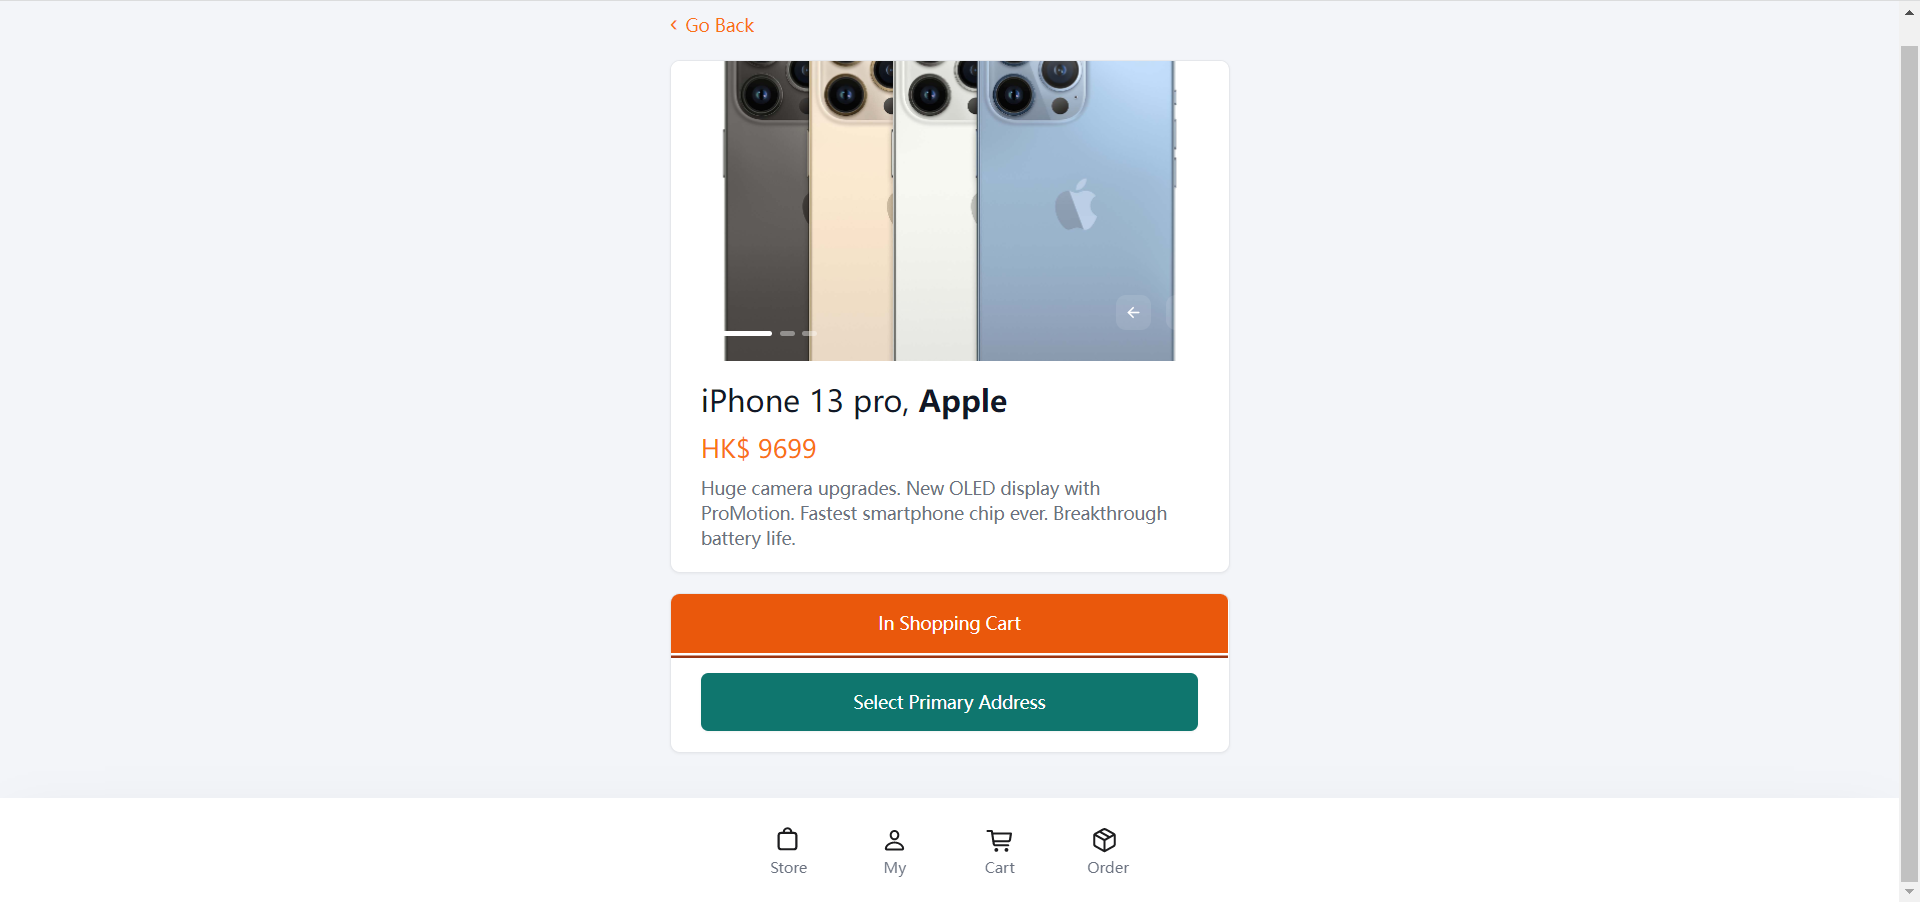
\includegraphics[width=0.6\textwidth]{Add in shopping_cart.png}
    \caption{\label{fig:add in shopping_cart} Add to the shopping cart successfully}
\end{figure}
\\\\
Another one is if the user is not login, the system will directly redirect to the login page. Users need to login with the email address and password and the system will redirect the user bach to the original product detail page to add the product to the shopping cart.

\subsubsection{Customer-Registration}
If they do not want to ship the product to the address in the current address, they can click the green button [see Figure \ref{fig:add in shopping_cart}] which will jump to the address management page [see Figure \ref{fig:manage address}]. On this page, users can add new addresses and select the primary address.
\begin{figure}[!htp]
    \centering
    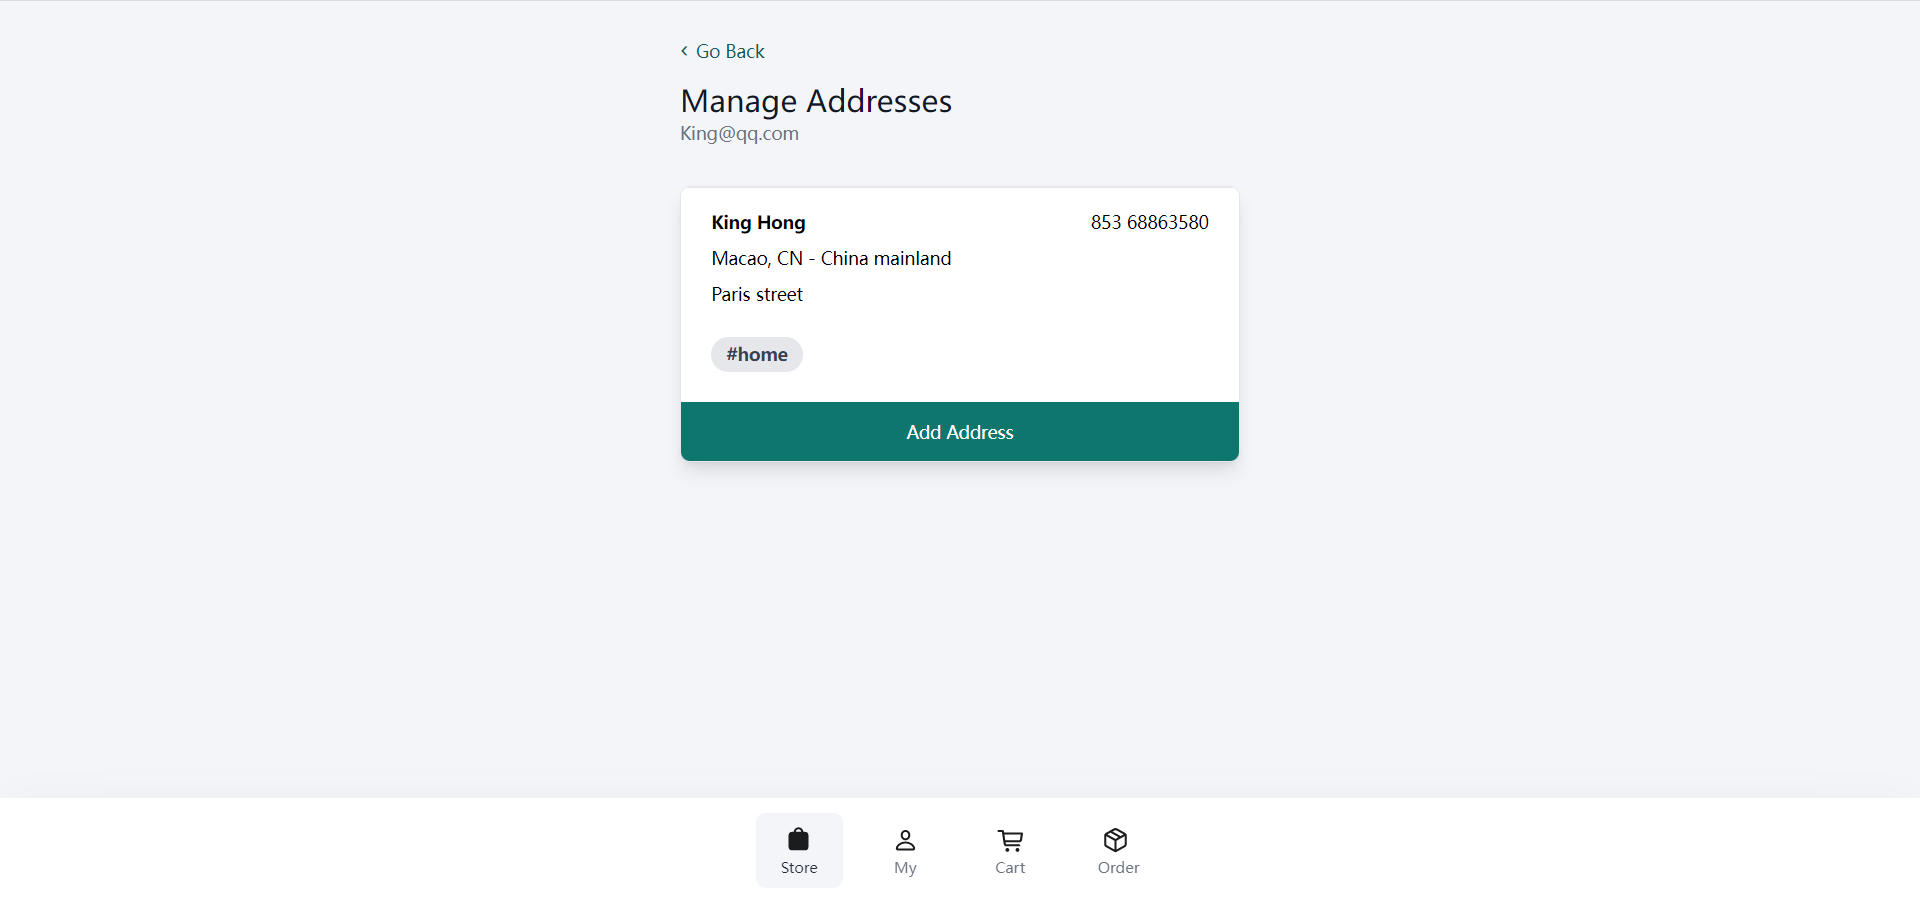
\includegraphics[width=0.6\textwidth]{manage address.png}
    \caption{\label{fig:manage address} Address management page}
\end{figure}
\\\\
When users want to buy the product on our platform, they will need to register their accounts. On the register page [see Figure \ref{fig:register}], there are two steps. In the first step, users have to provide a user name, email address, and password. Password need at least 6 letters, in particular, it needs at least one capital letter. Users also need to read the user policy and agree with that.  
\begin{figure}[!htp]
    \centering
    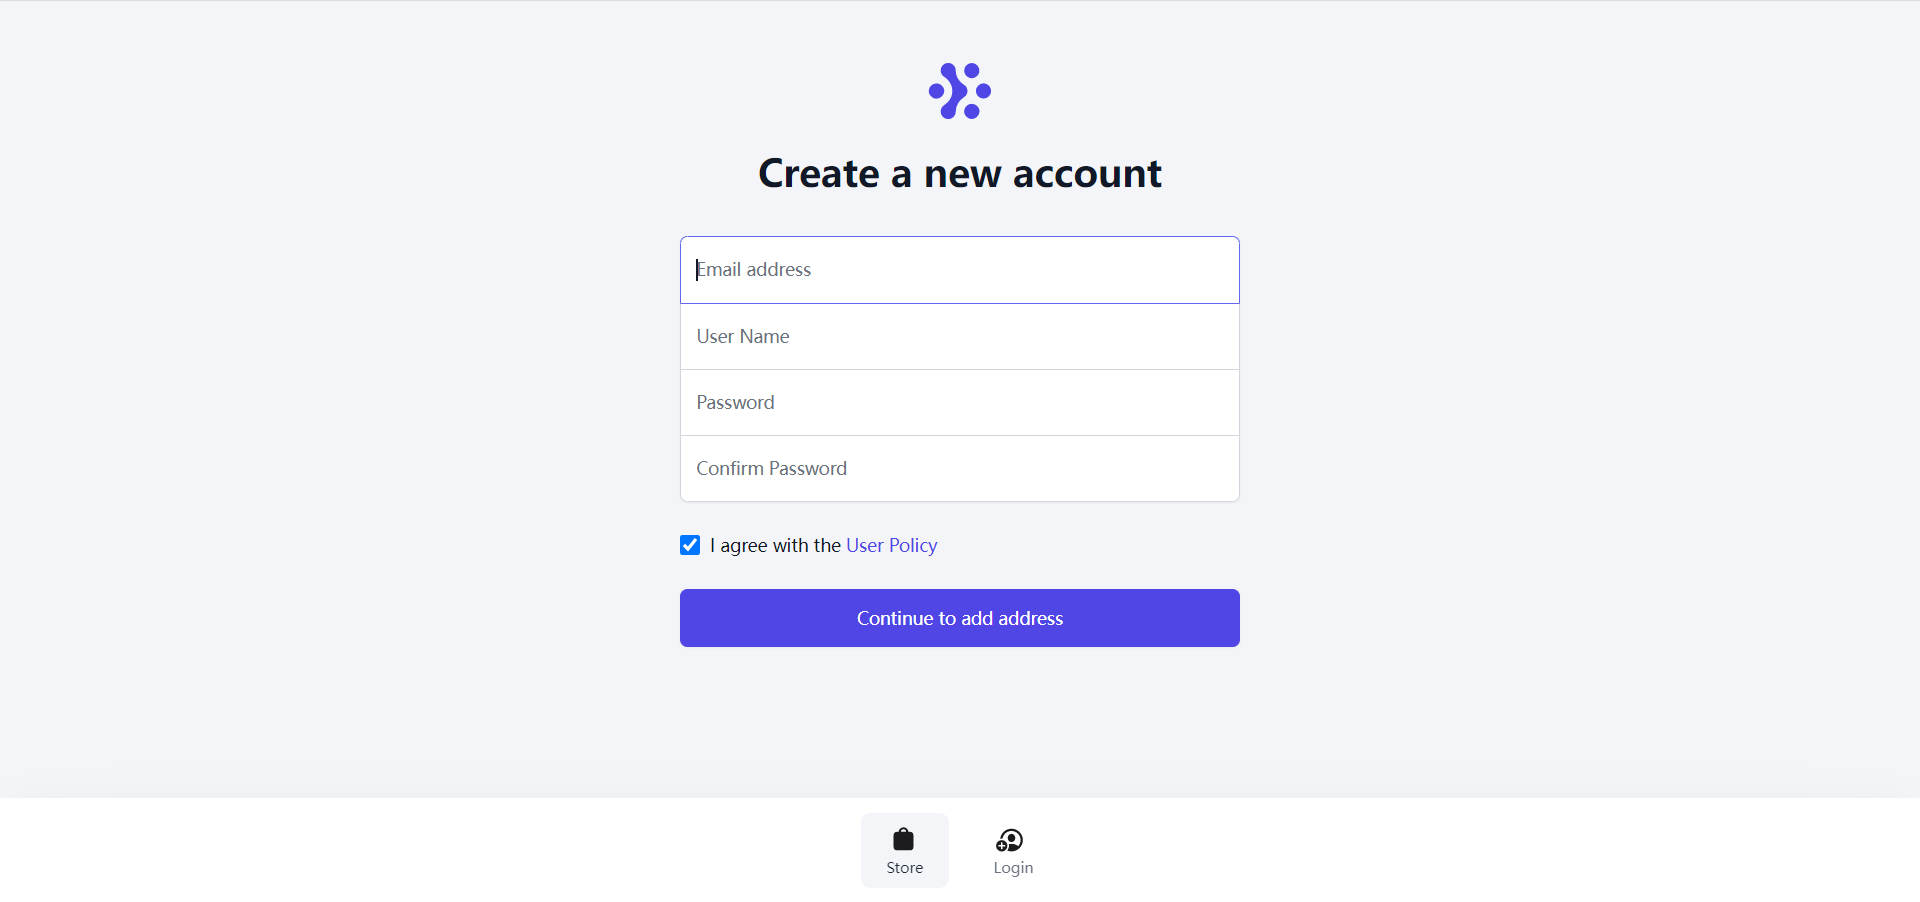
\includegraphics[width=0.6\textwidth]{register.png}
    \caption{\label{fig:register}Register page}
\end{figure}
\\\\
The second step is adding an address [see Figure \ref{fig:add address}]. Users have to provide their first name, last name, phone number, and address. In addition, they can put a tag on this address to helping to manage addresses.
\begin{figure}[!htp]
    \centering
    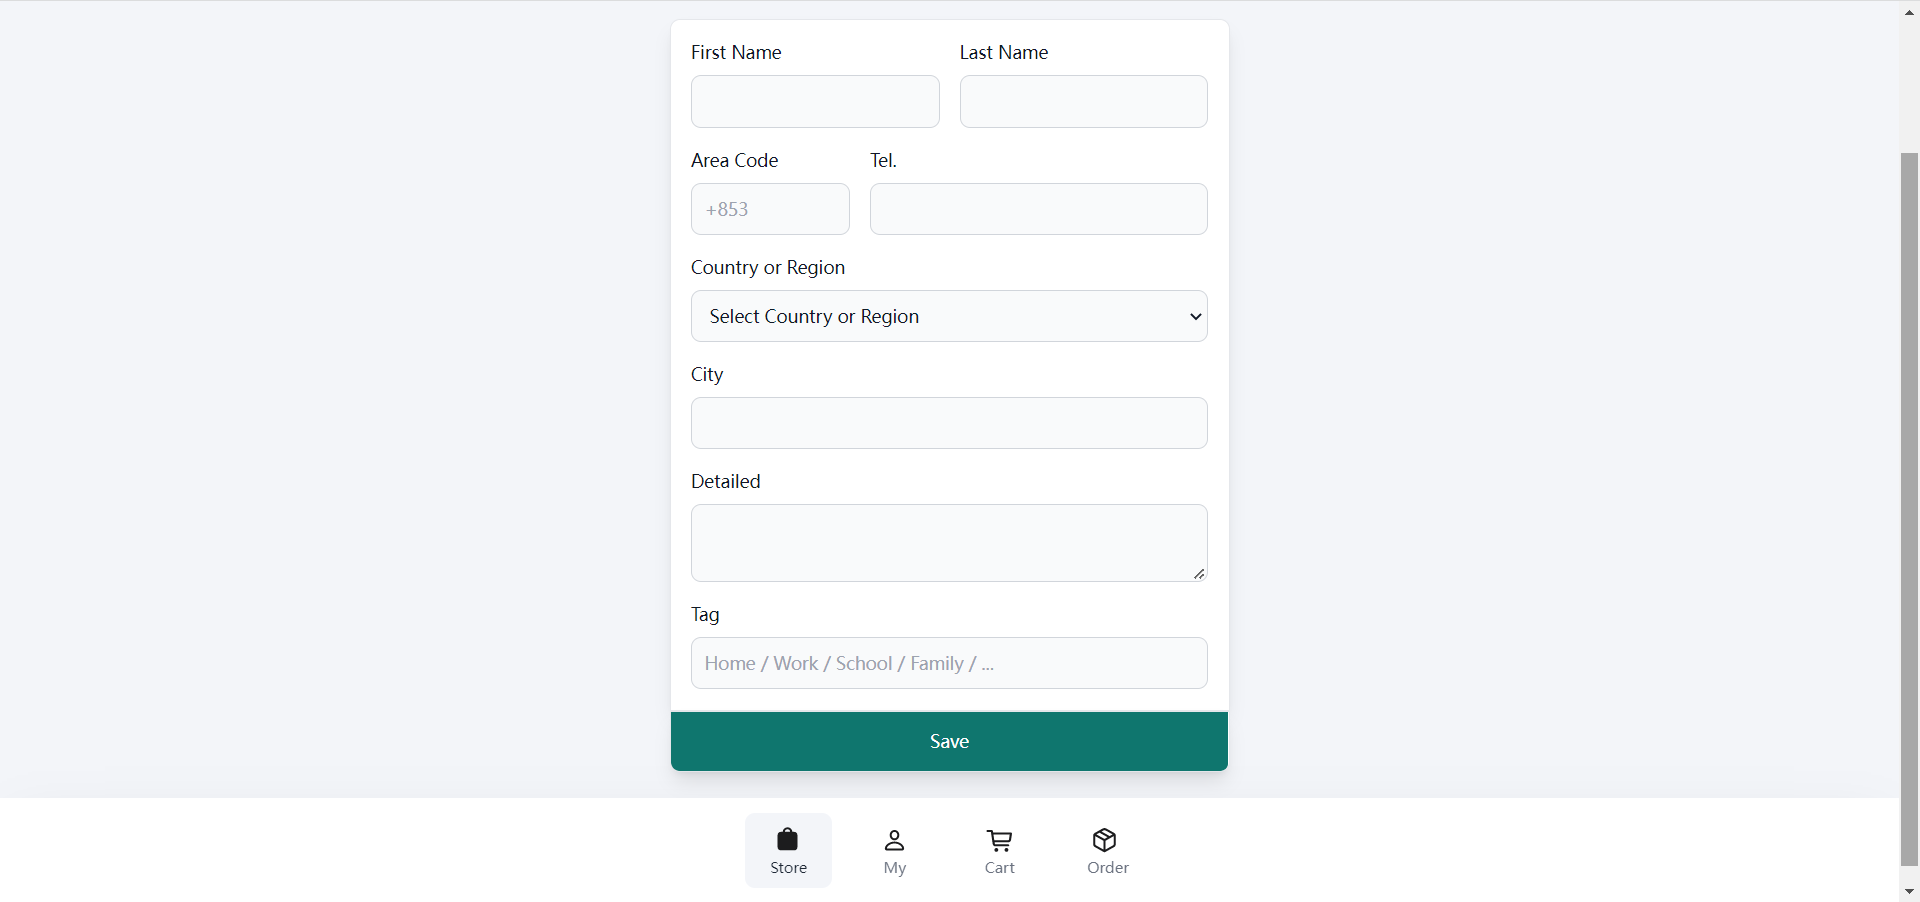
\includegraphics[width=0.6\textwidth]{add address.png}
    \caption{\label{fig:add address} Adding address page }
\end{figure}
When users successfully register, the system will automatically help users to log in and jump to the account management page [see Figure \ref{fig:account management page}].
\begin{figure}[!htp]
    \centering
    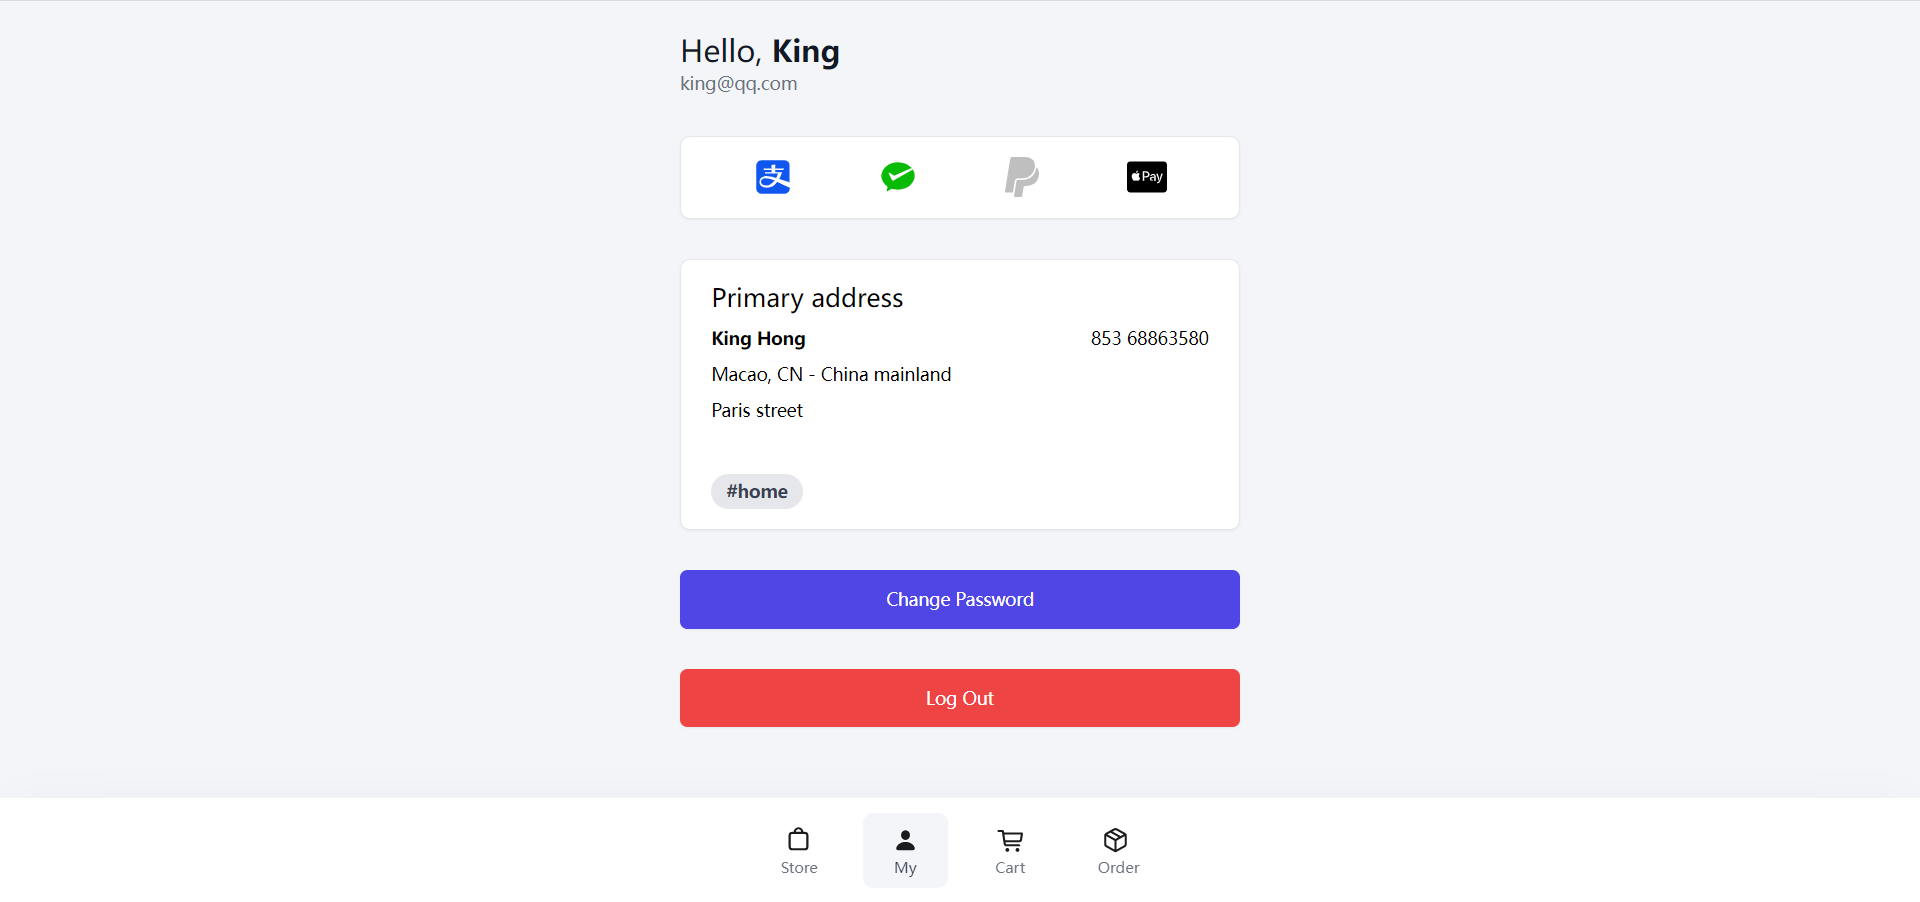
\includegraphics[width=0.6\textwidth]{account management.png}
    \caption{\label{fig:account management page} Account management page}
\end{figure}

\subsubsection{Customer-Shopping cart}
After users have finished browsing and selecting, the shopping cart function will be provided for them to check out. On the shopping cart page [see Figure \ref{fig:shopping cart page}], users can list the products in their shopping cart. The entry for each product shows the product name, price, and the quantity to buy. The page also shows the total order amount in the shopping cart. The user can click an item in the shopping cart to go to the product detail page of the entry. User can remove the item or change the quantity of an item. But the most important function of this page is that users can press the button “Checkout” to check out all items in the shopping cart. Here is a very user-friendly design. When the user adds a duplicate product to the shopping cart, the system will give a warning message and does not change the content of the shopping cart.
\begin{figure}[!htp]
    \centering
    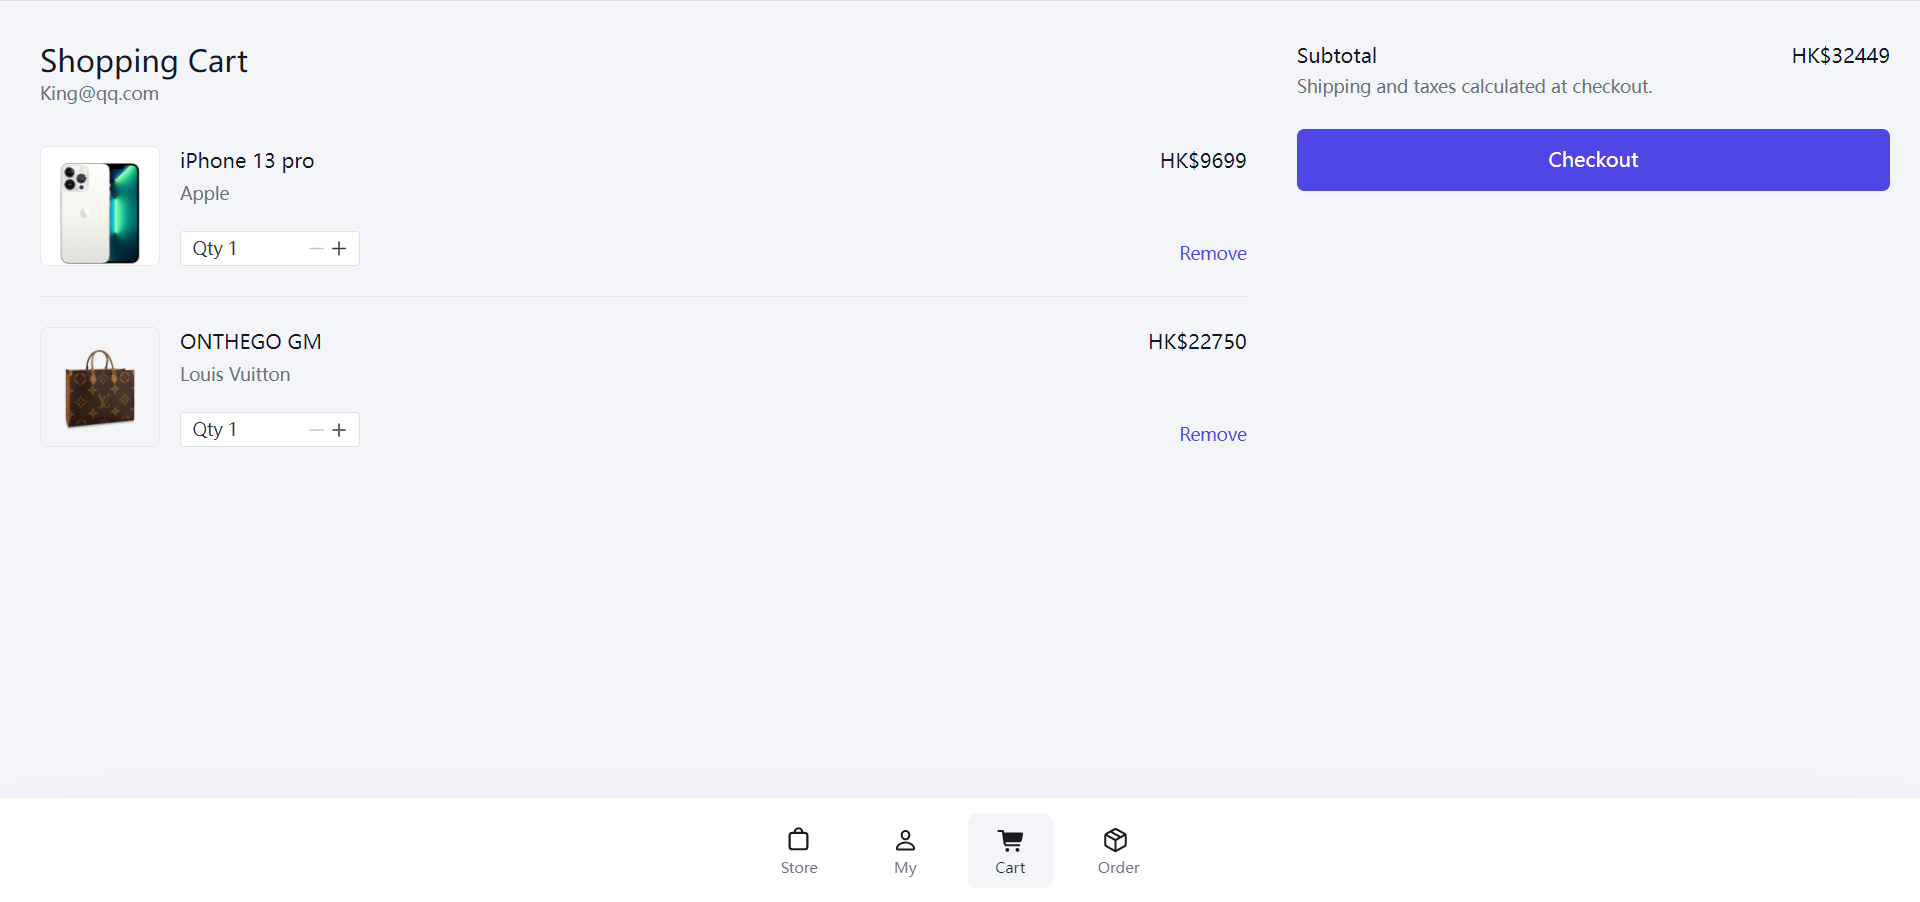
\includegraphics[width=0.6\textwidth]{shopping cart page.png}
    \caption{\label{fig:shopping cart page} Shopping cart page}
\end{figure}
\\\\
After clicking the “Checkout” button, the system will create an order [see Figure \ref{fig:order detail page}] including the product name, price, and the quantity to buy. After checking the content of the order, if there is no error about the content, users can click the “Pay” button to pay for the order. If there is an error in the content, the user can click “Go Back” to check the shopping cart again.
\begin{figure}[!htp]
    \centering
    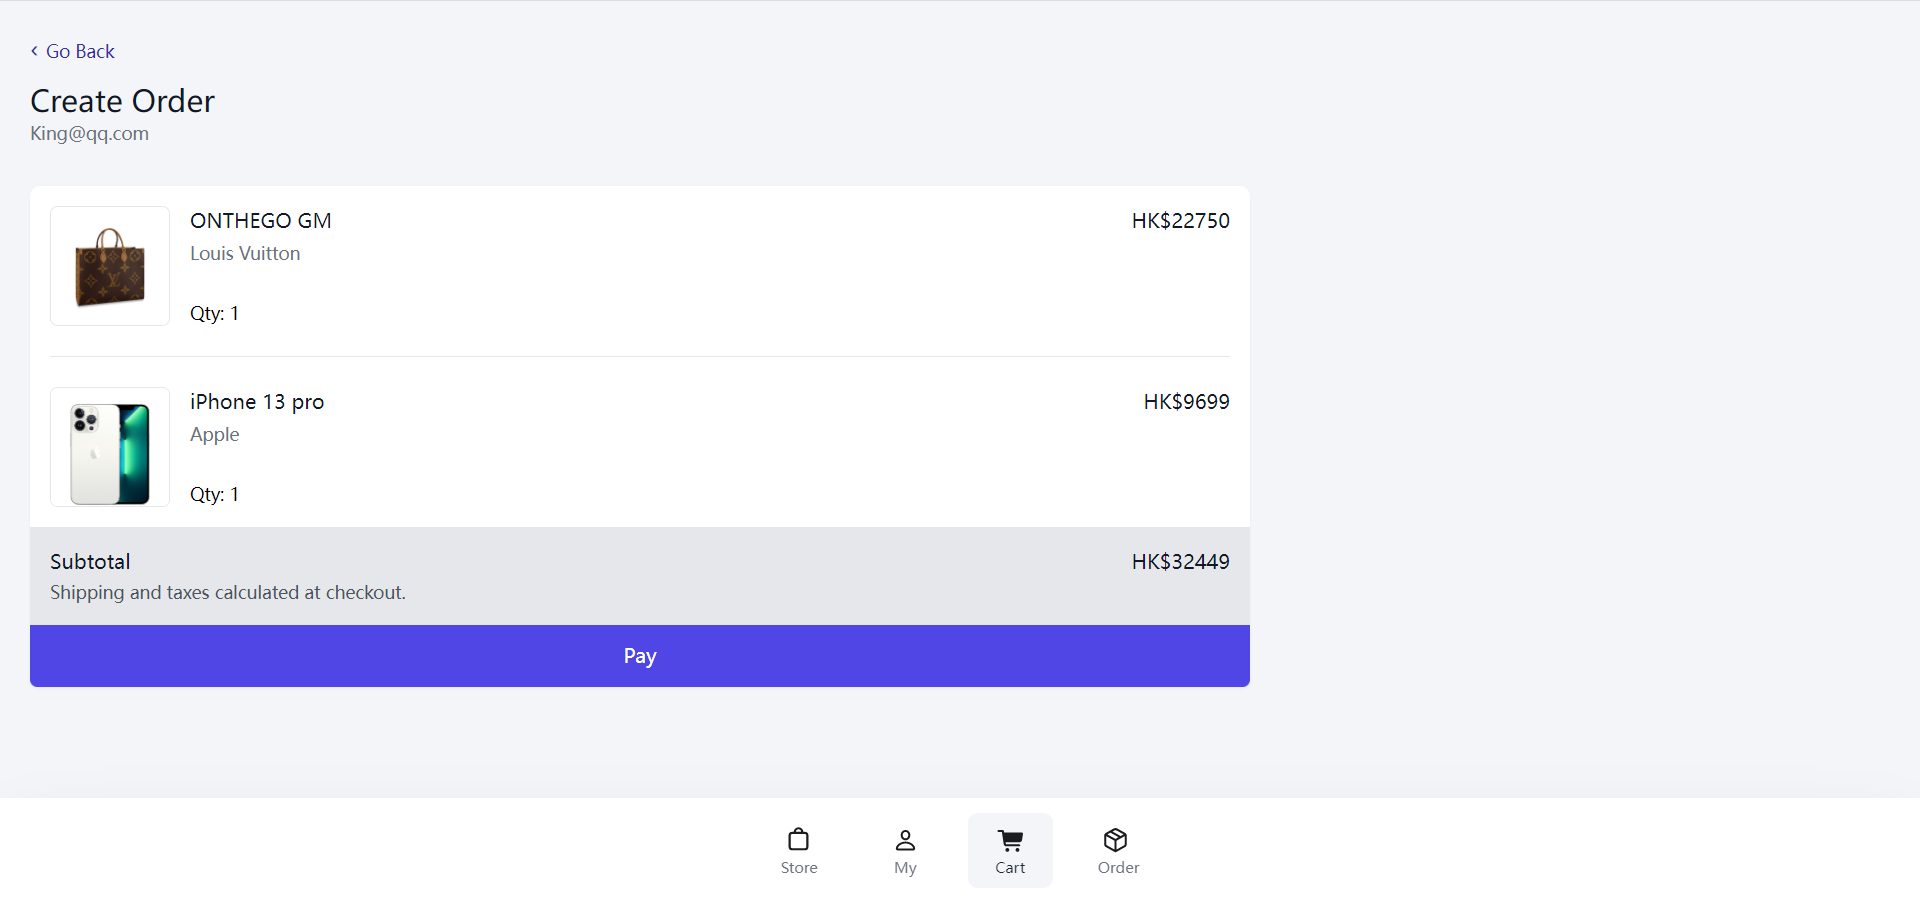
\includegraphics[width=0.6\textwidth]{order detail page.png}
    \caption{\label{fig:order detail page}Order detail pgae}
\end{figure}
\\\\
Once paying is finished, the system will create a purchase order [see Figure \ref{fig:purchase detail page}] with a newly allocated unique P.O. number and clears the content of the cart. Then the system will show the purchase order detail page of the newly created purchase order. The purchase order detail page shows the P.O. number, the purchase date, the customer name, the shipping address, the total order amount, and the purchases order status. The page also includes, for each product in the purchase order, the product name, the quantity, the unit price, and the subtotal. 
\begin{figure}[!htp]
    \centering
    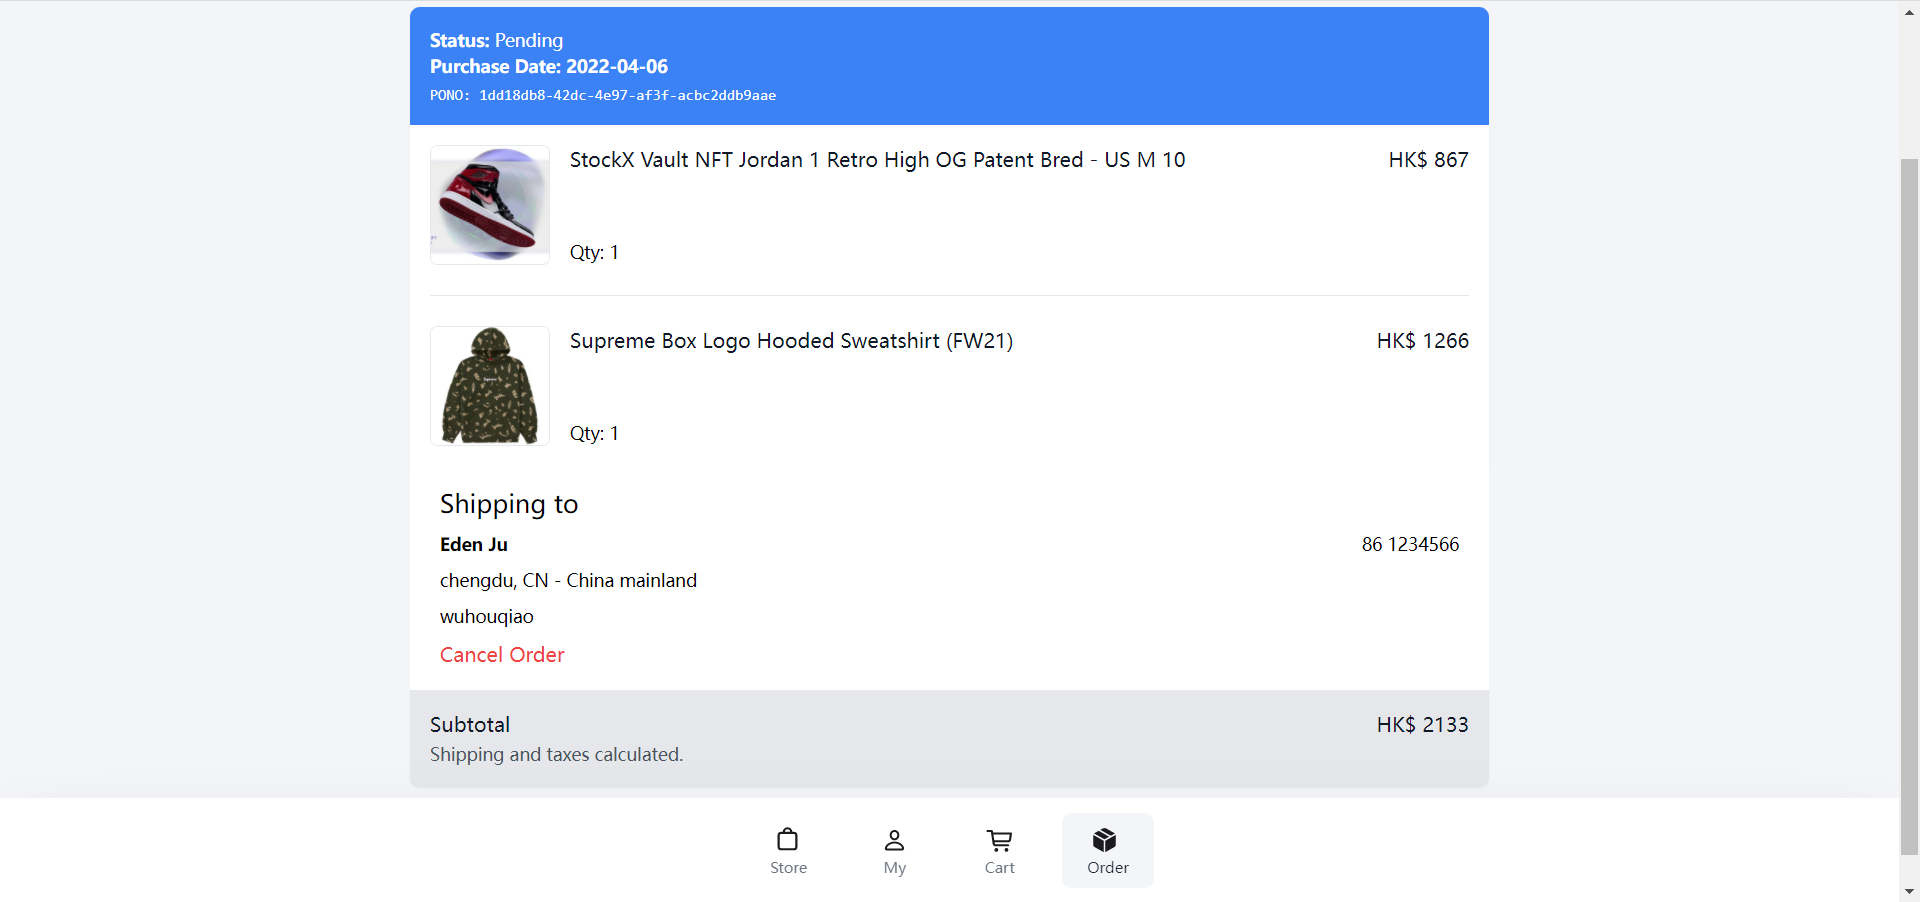
\includegraphics[width=0.6\textwidth]{purchase detail page.png}
    \caption{\label{fig:purchase detail page}Purchase detail page }
\end{figure}

\subsubsection{Customer-Purchase tracking}
The User can trace the processing status of the order on the purchase tracking page [see Figure \ref{fig:purchase list}]. The purchase tracking page lists the purchase orders that the user has placed. This page shows the following for each purchase order: the P.O. number, the purchase date, the total order amount, and the purchase order status. The purchase orders are displayed in reverse chronological order of purchase date. When the user clicks an entry in the list, they can see the detail in a purchase order detail page.
\begin{figure}[!htp]
    \centering
    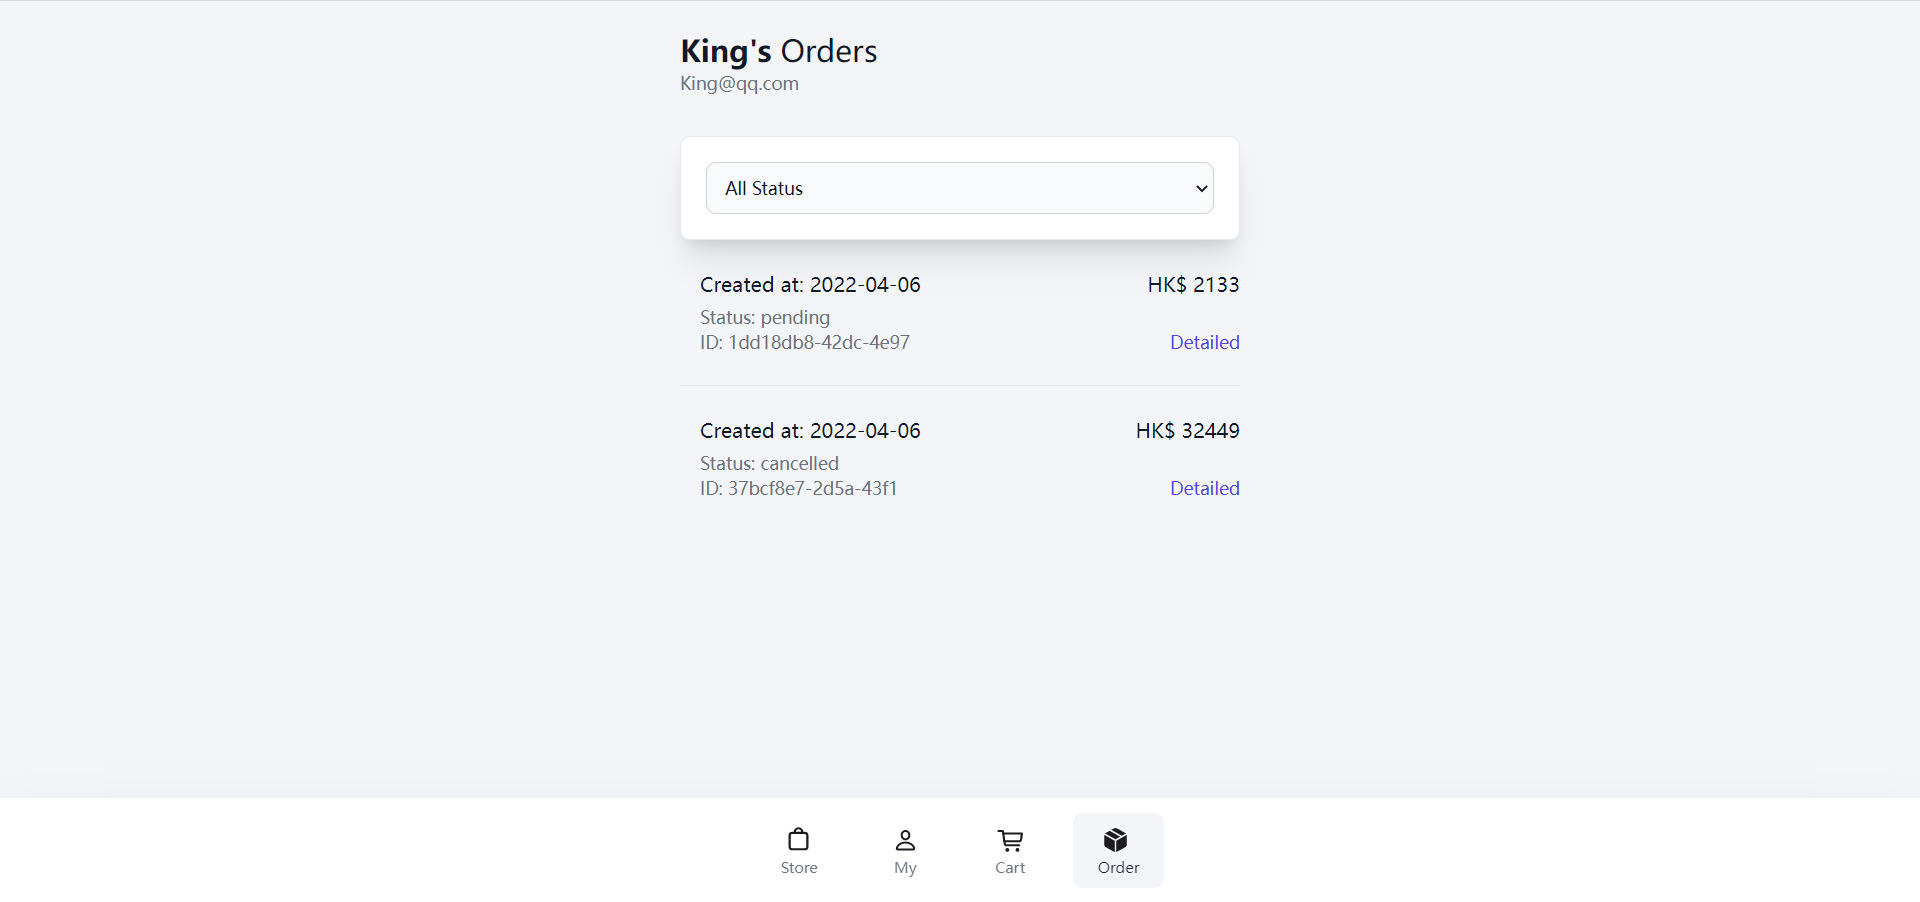
\includegraphics[width=0.6\textwidth]{purchase list.png}
    \caption{\label{fig:purchase list} Purchase list}
\end{figure}
\\\\
Before a purchase order is shipped, the customer can cancel the order. This can be done by clicking a button on the purchase order detail page [see Figure \ref{fig:order detail page}].
\\\\
There are a few differences in the user interface between login and not log in. The first difference is the user name will be displayed in the interface [see Figure \ref{fig:logined product list } and \ref{fig:product list}]. The second difference is the navigation bar. Logged-in users can browse shopping carts, manage accounts, and browse order lists. Users who do not login can only browse the product list and log in.
\begin{figure}[!htp]
    \centering
    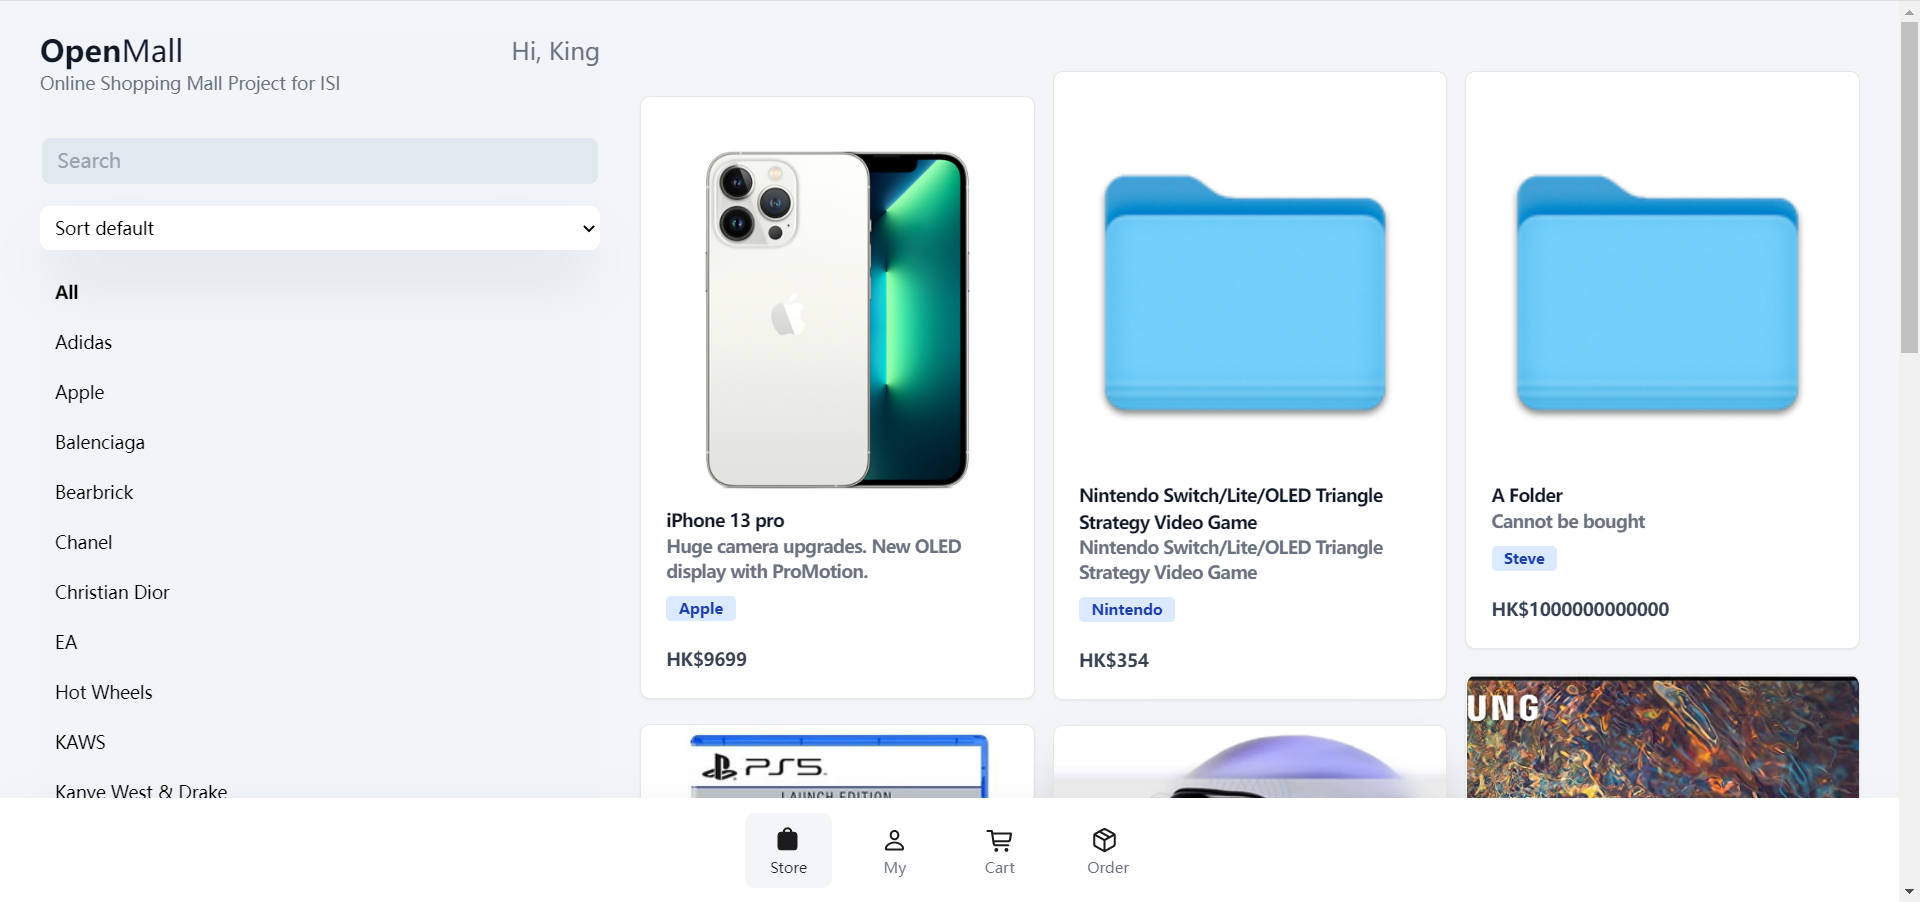
\includegraphics[width=0.6\textwidth]{logined product list.png}
    \caption{\label{fig:logined product list }Main interface for the login customer}
\end{figure}

\newpage
\subsubsection{Vendor}
The vendor can maintain product catalogue in the shopping mall and process purchase orders from customers as well. 
\begin{figure}[!htp]
    \centering
    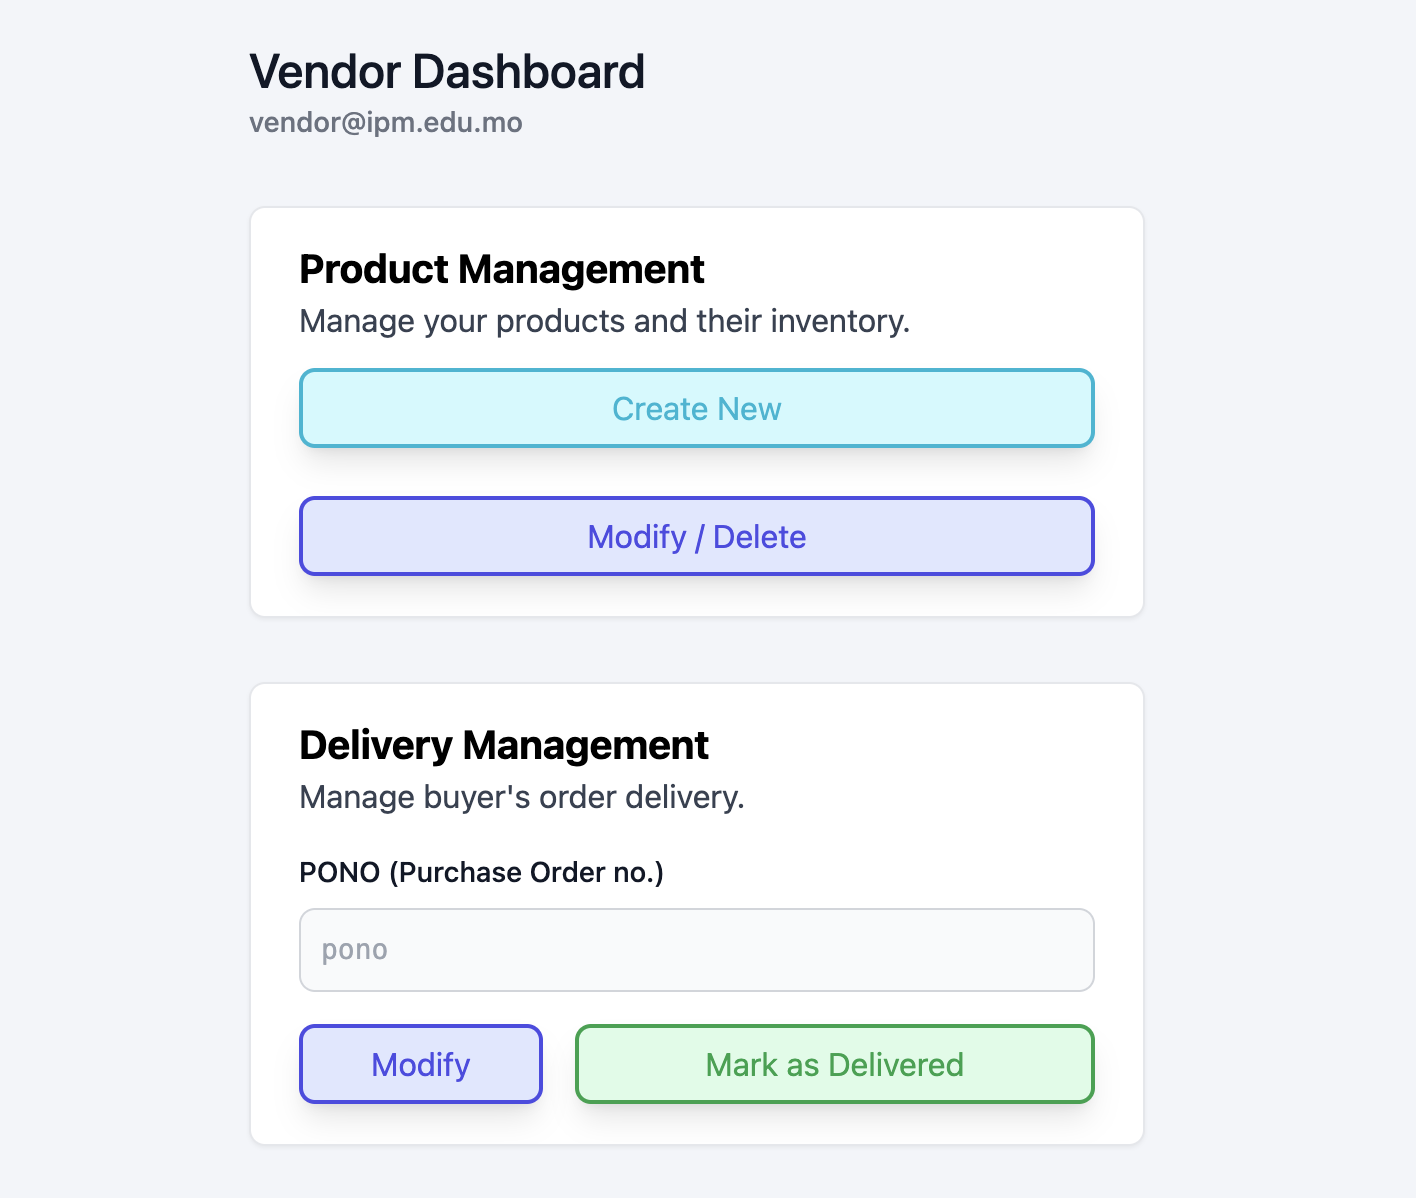
\includegraphics[width=0.6\textwidth]{vendor outlook.png}
    \caption{\label{fig:vendor outlook}Main interface for the Vendor}
\end{figure}

\subsubsection{Vendor-Product catalog management}
The first feature is product management. The vendor can create new product or modify current products in this field. With pressing “Create New” button, an empty list should the vendor type to upload necessary information including product name, brand, price, a thumbnail image, 1 to 4 detailed photographs and some detailed information in order to create a new product. 
\begin{figure}[htbp]
\centering
\begin{minipage}[t]{0.48\textwidth}
\centering
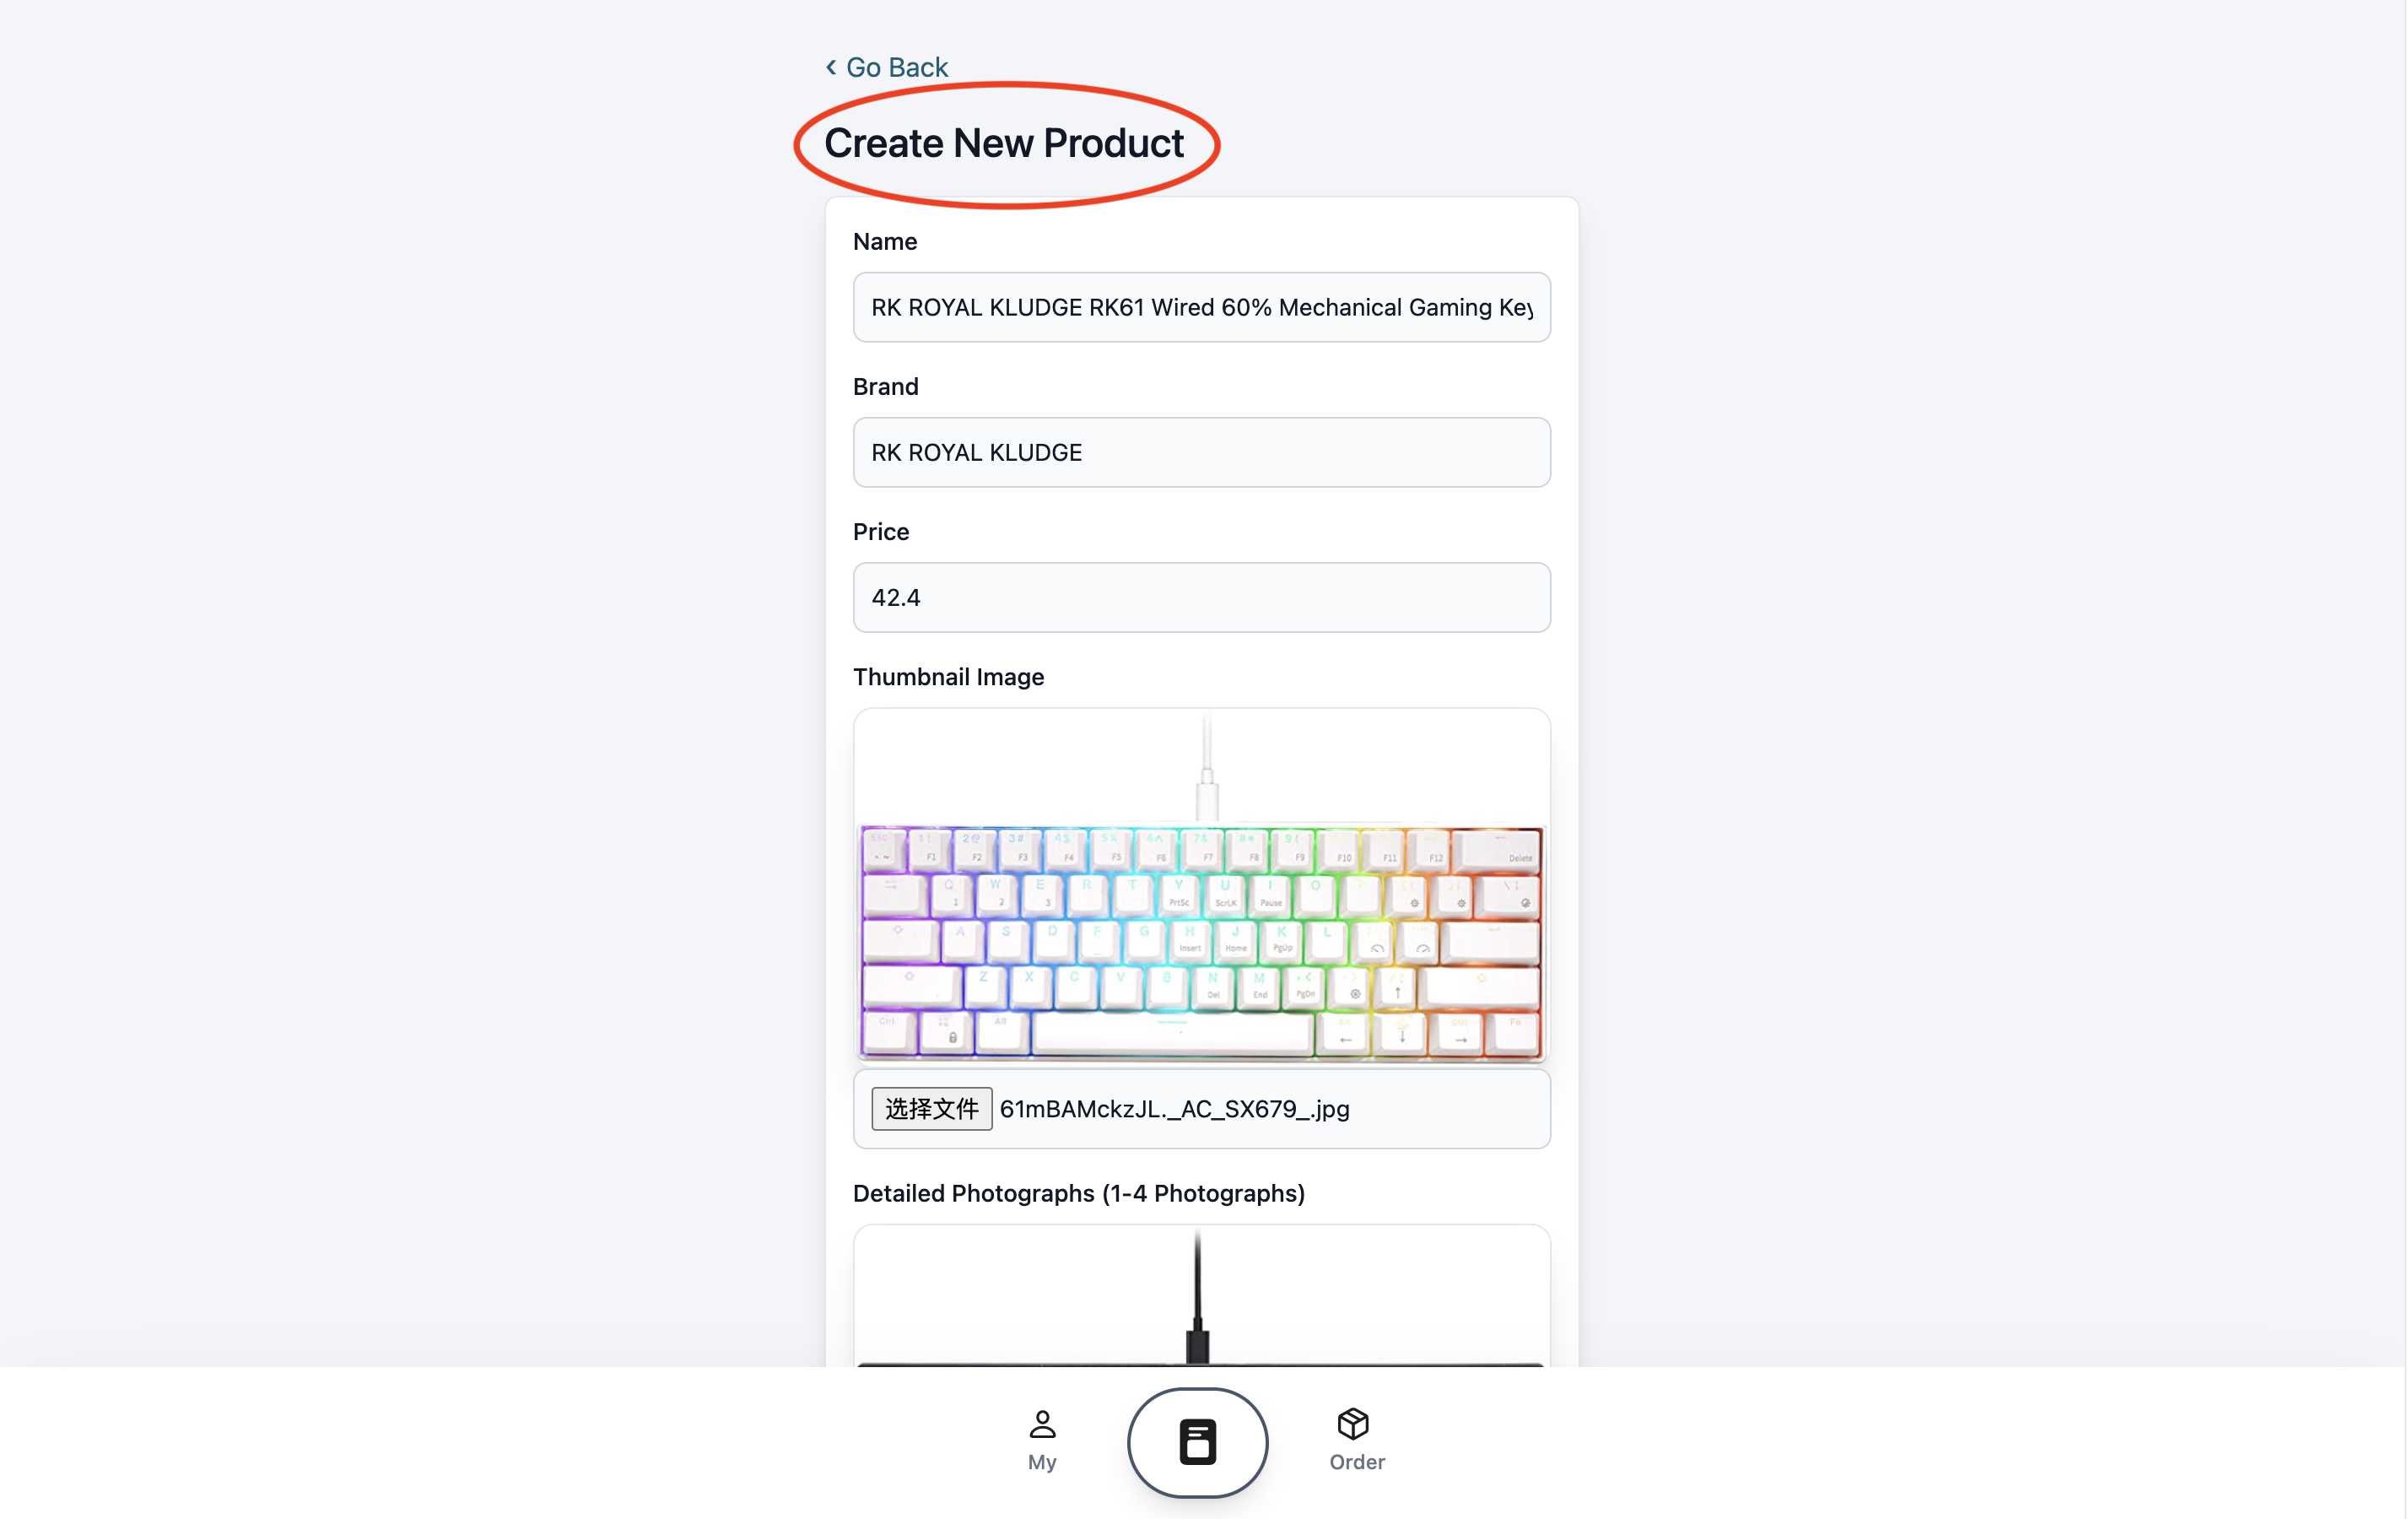
\includegraphics[width=6cm]{create example 1.png}
\caption{Vendor create a product}
\end{minipage}
\begin{minipage}[t]{0.48\textwidth}
\centering
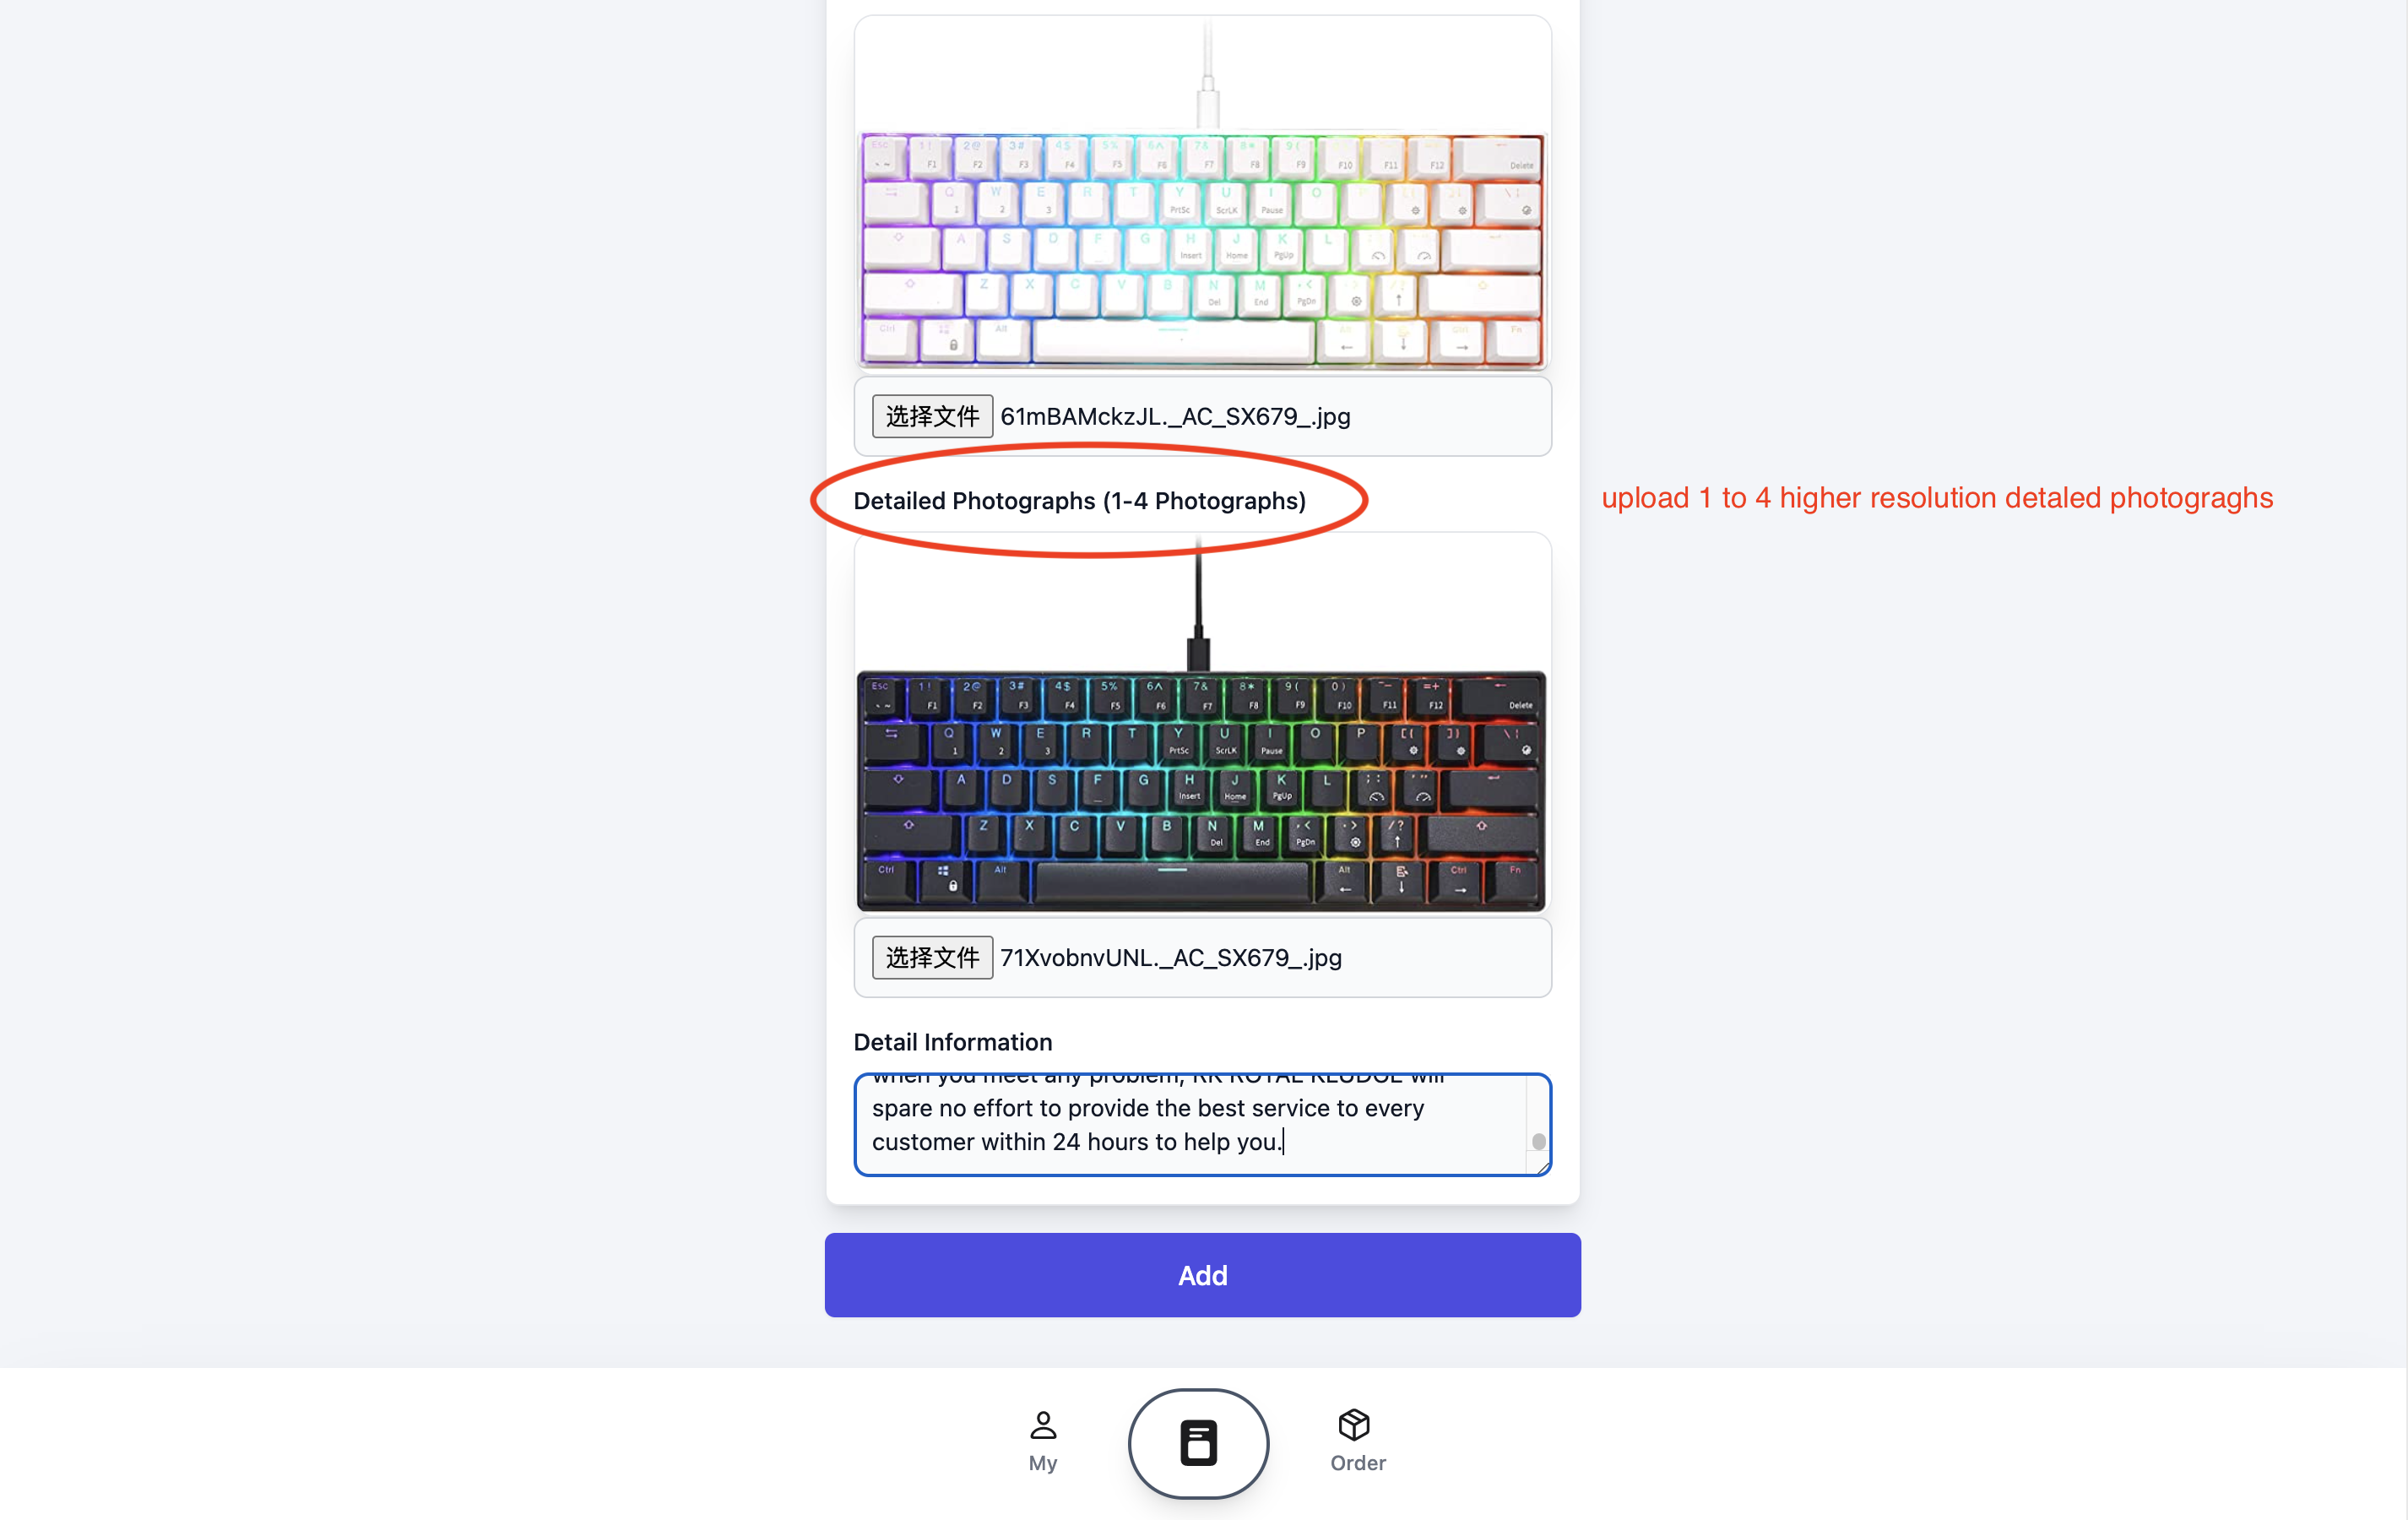
\includegraphics[width=6cm]{create example 2.png}
\caption{The confirmation and the error message}
\end{minipage}
\end{figure}
\newpage
\leavevmode
\\\\
Any missing data will result in a relevant message being displayed. 
\begin{figure}[!htp]
    \centering
    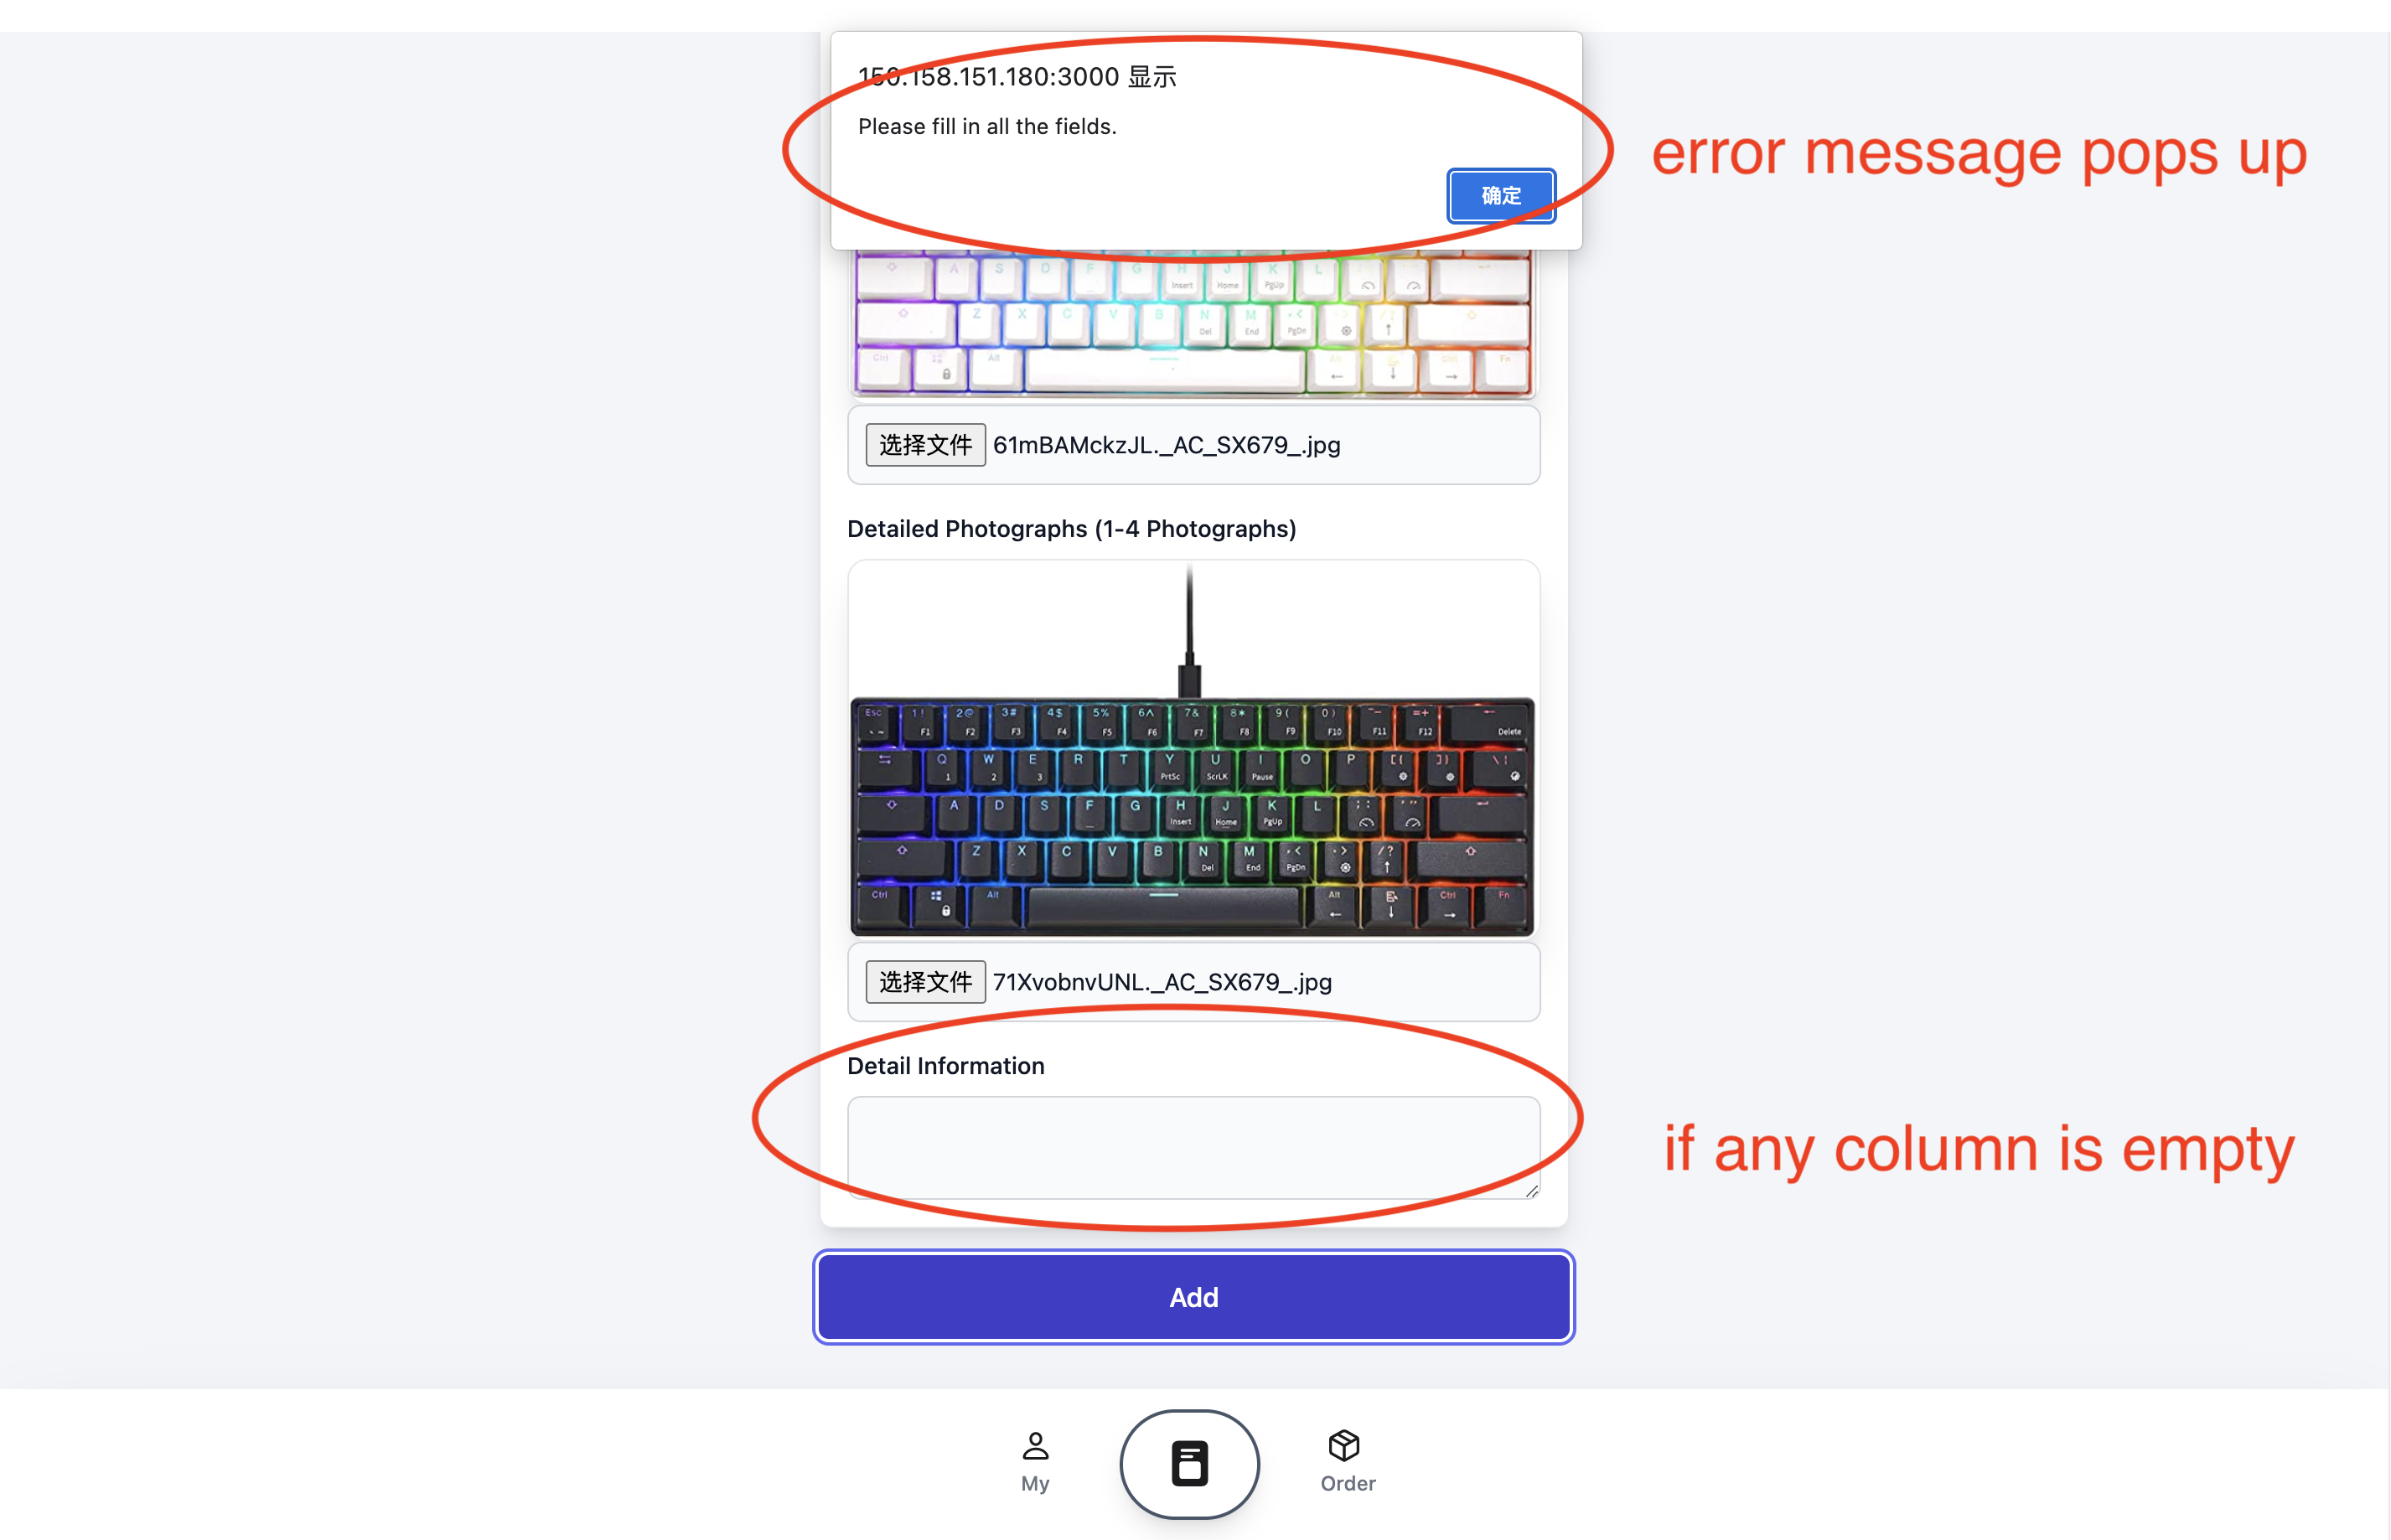
\includegraphics[width=0.72\textwidth]{error message.png}
    \caption{\label{fig:error message}Error message if product cannot be created}
\end{figure}
\\\\
If a new product is created successfully, the vendor can press the "Edit The Product" to do further modifications. (see Figure \ref{fig:successfully create})
\begin{figure}[!htp]
    \centering
    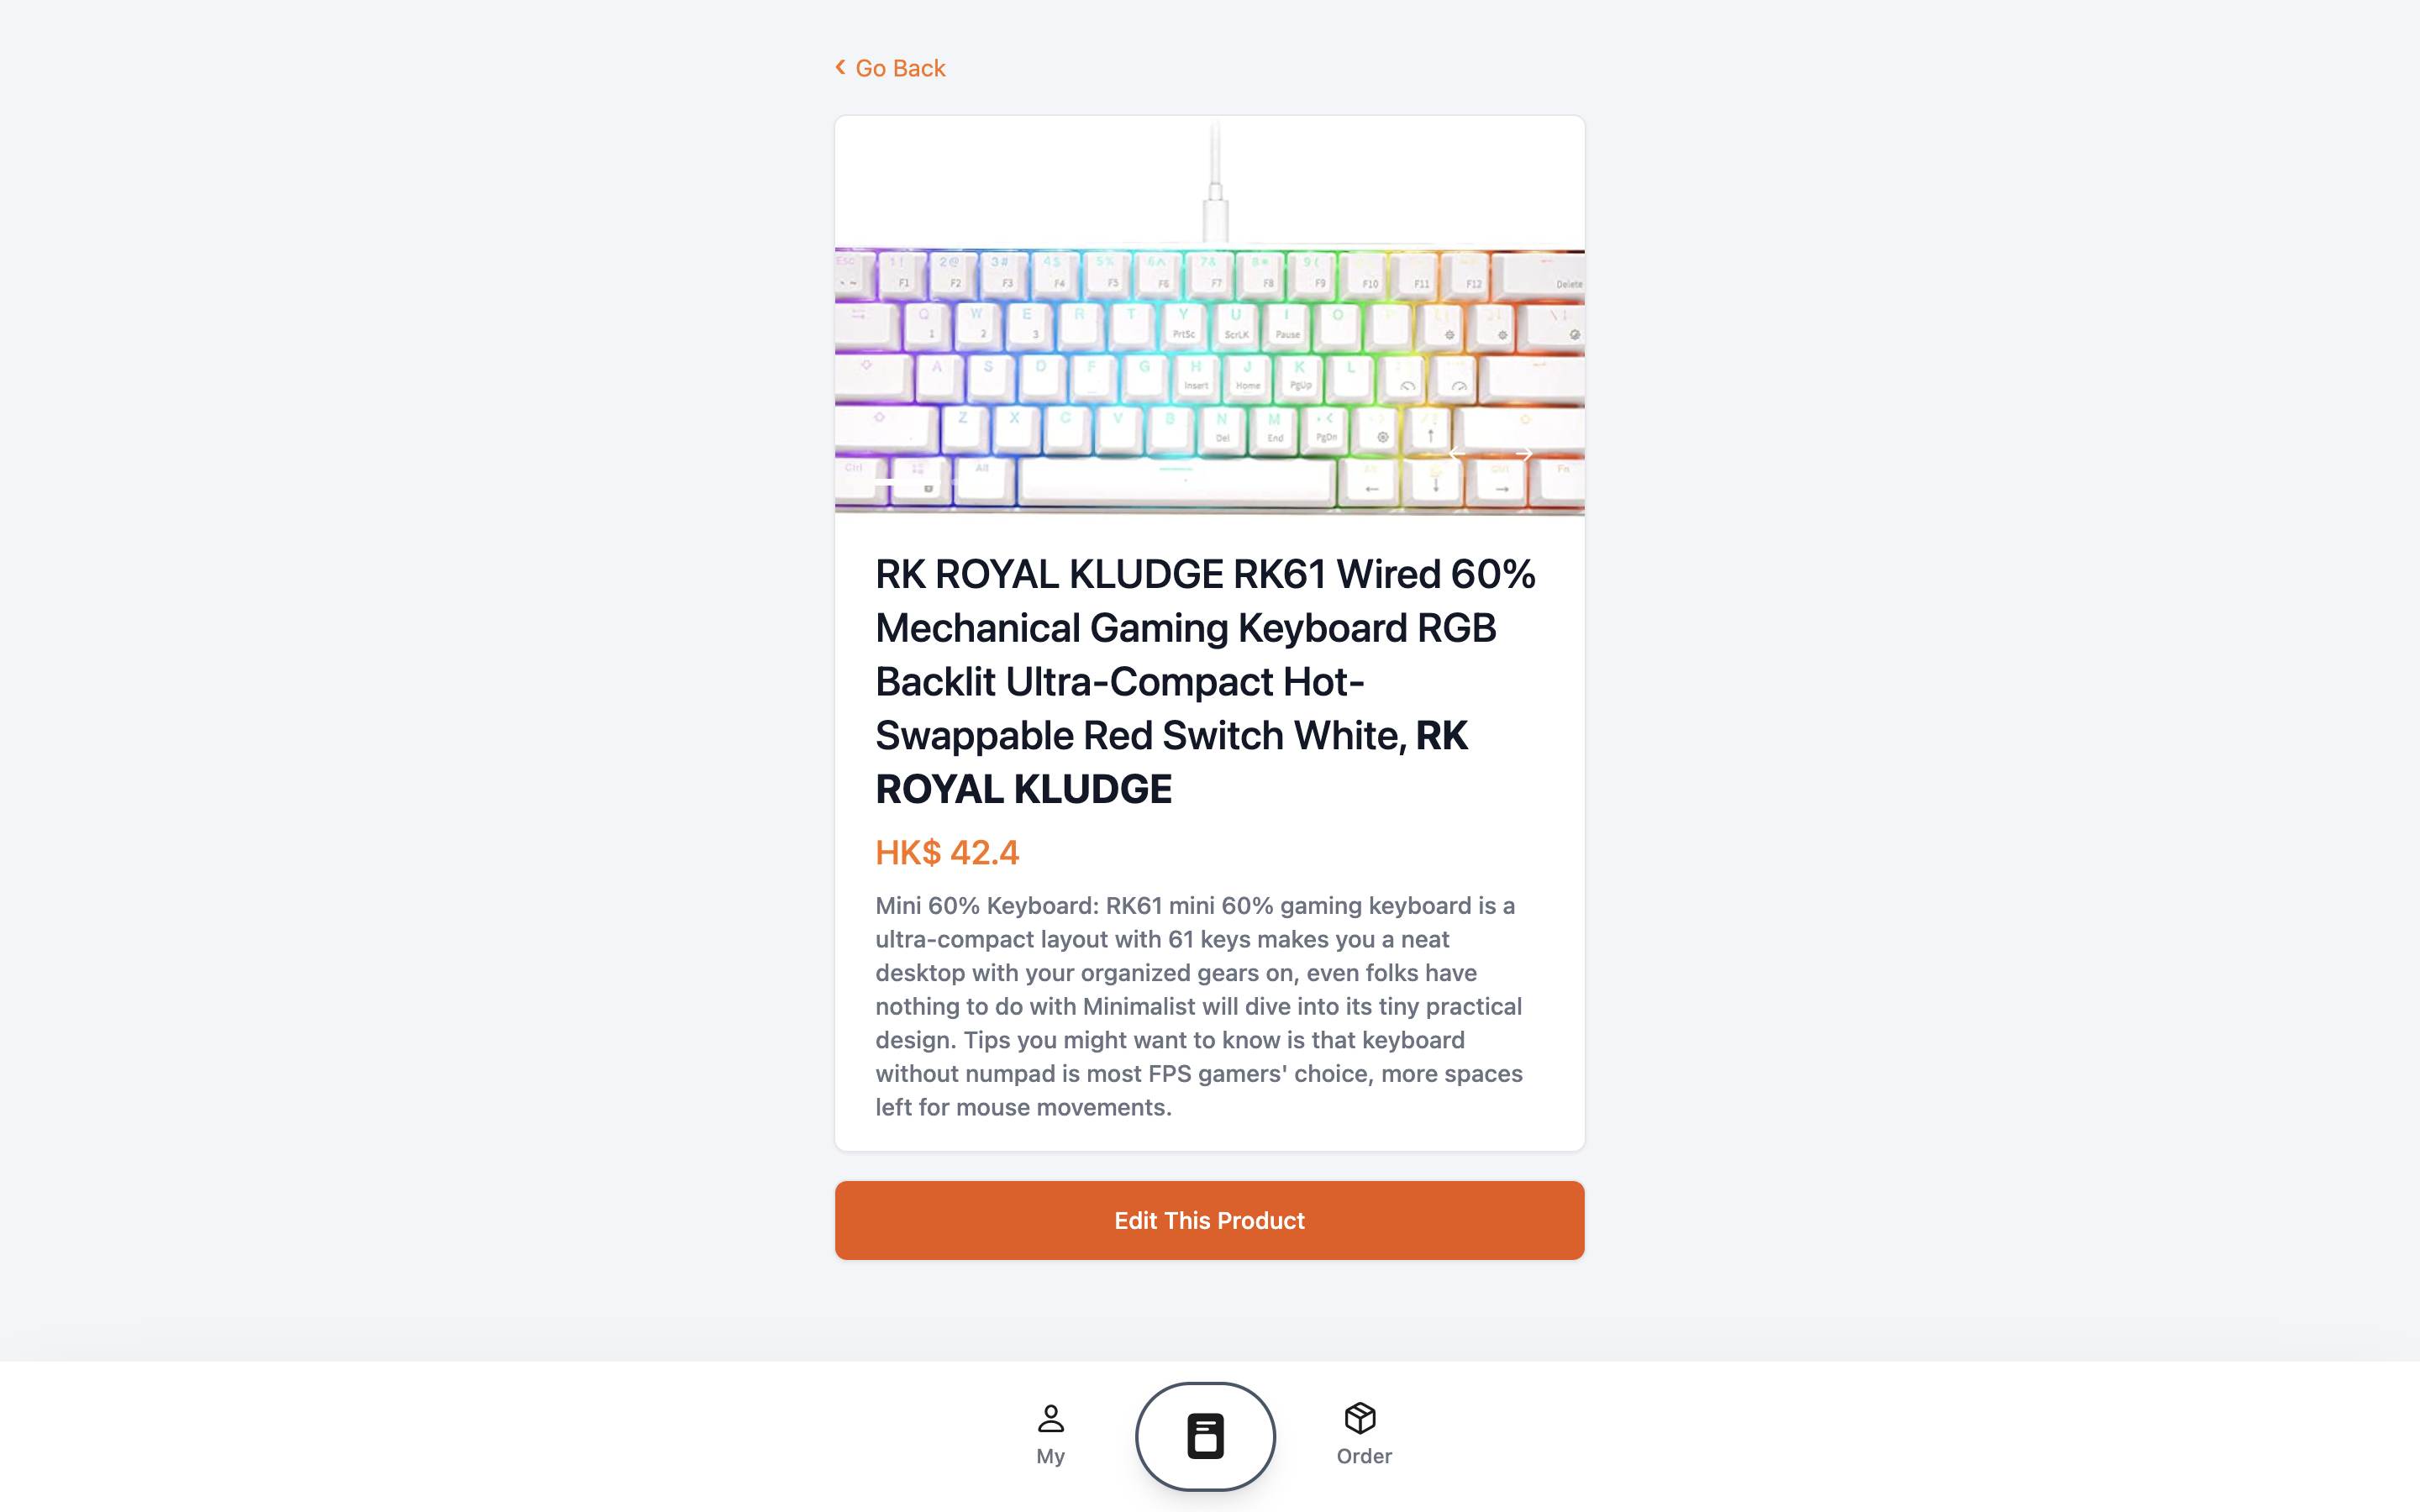
\includegraphics[width=0.72\textwidth]{create successfully.png}
    \caption{\label{fig:successfully create}An added product can be edited}
\end{figure}
\newpage
\leavevmode
\\\\
The product update list just looks like the one for creating new product. The vendor should guarantee all the columns are filled correctly, otherwise the same error message will displayed.(see Figure\ref{fig:Product update page})
\begin{figure}[htbp]
    \centering
    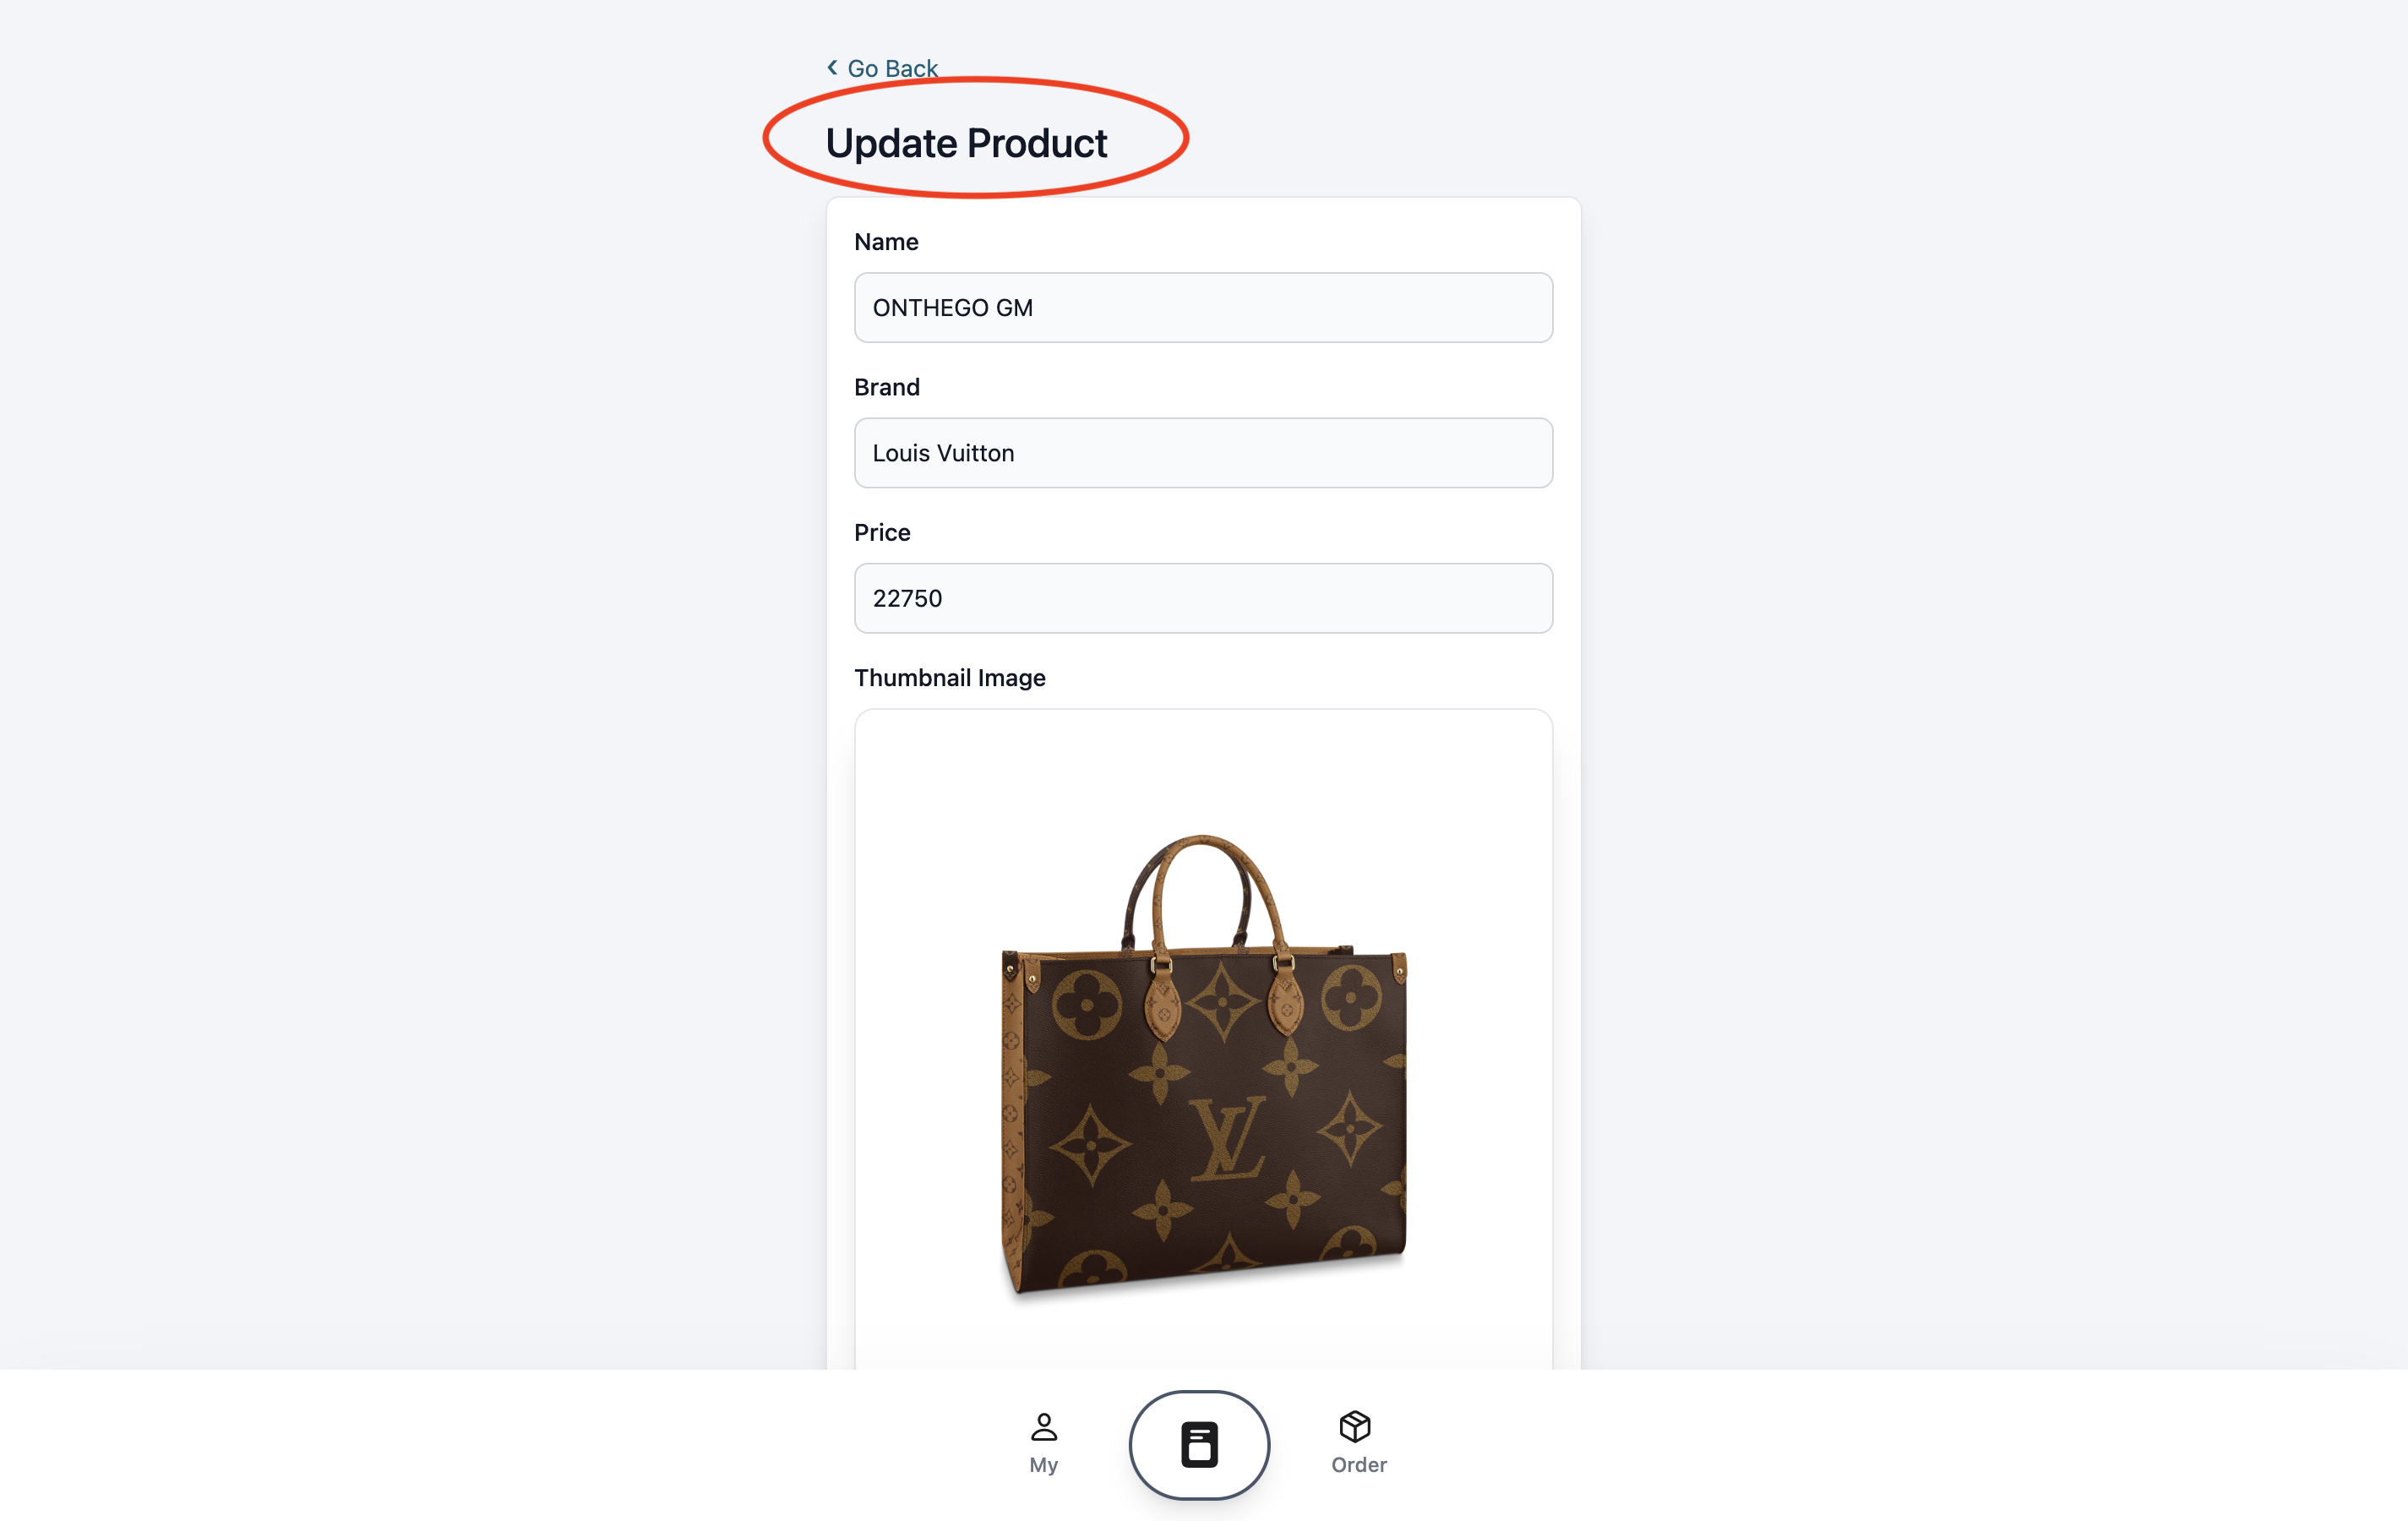
\includegraphics[width=0.72\textwidth]{modification.png}
    \caption{\label{fig:Product update page}Product update page}
\end{figure}

\subsubsection{Vendor-Product delivery management}
The second feature is delivery management. The vendor can track and modify buyer’s order delivery status. The vendor can also mark an order as delivered with input specific purchase order number or check all the orders in a chronological order list by pressing “Modify”.
In this purchase order list page, the vendor can filter any order with specific order status. Some important information is shown in the block in this list including the P.O.numbers, purchase dates, customer names, total order amounts and purchase order status. 
\begin{figure}[!htp]
    \centering
    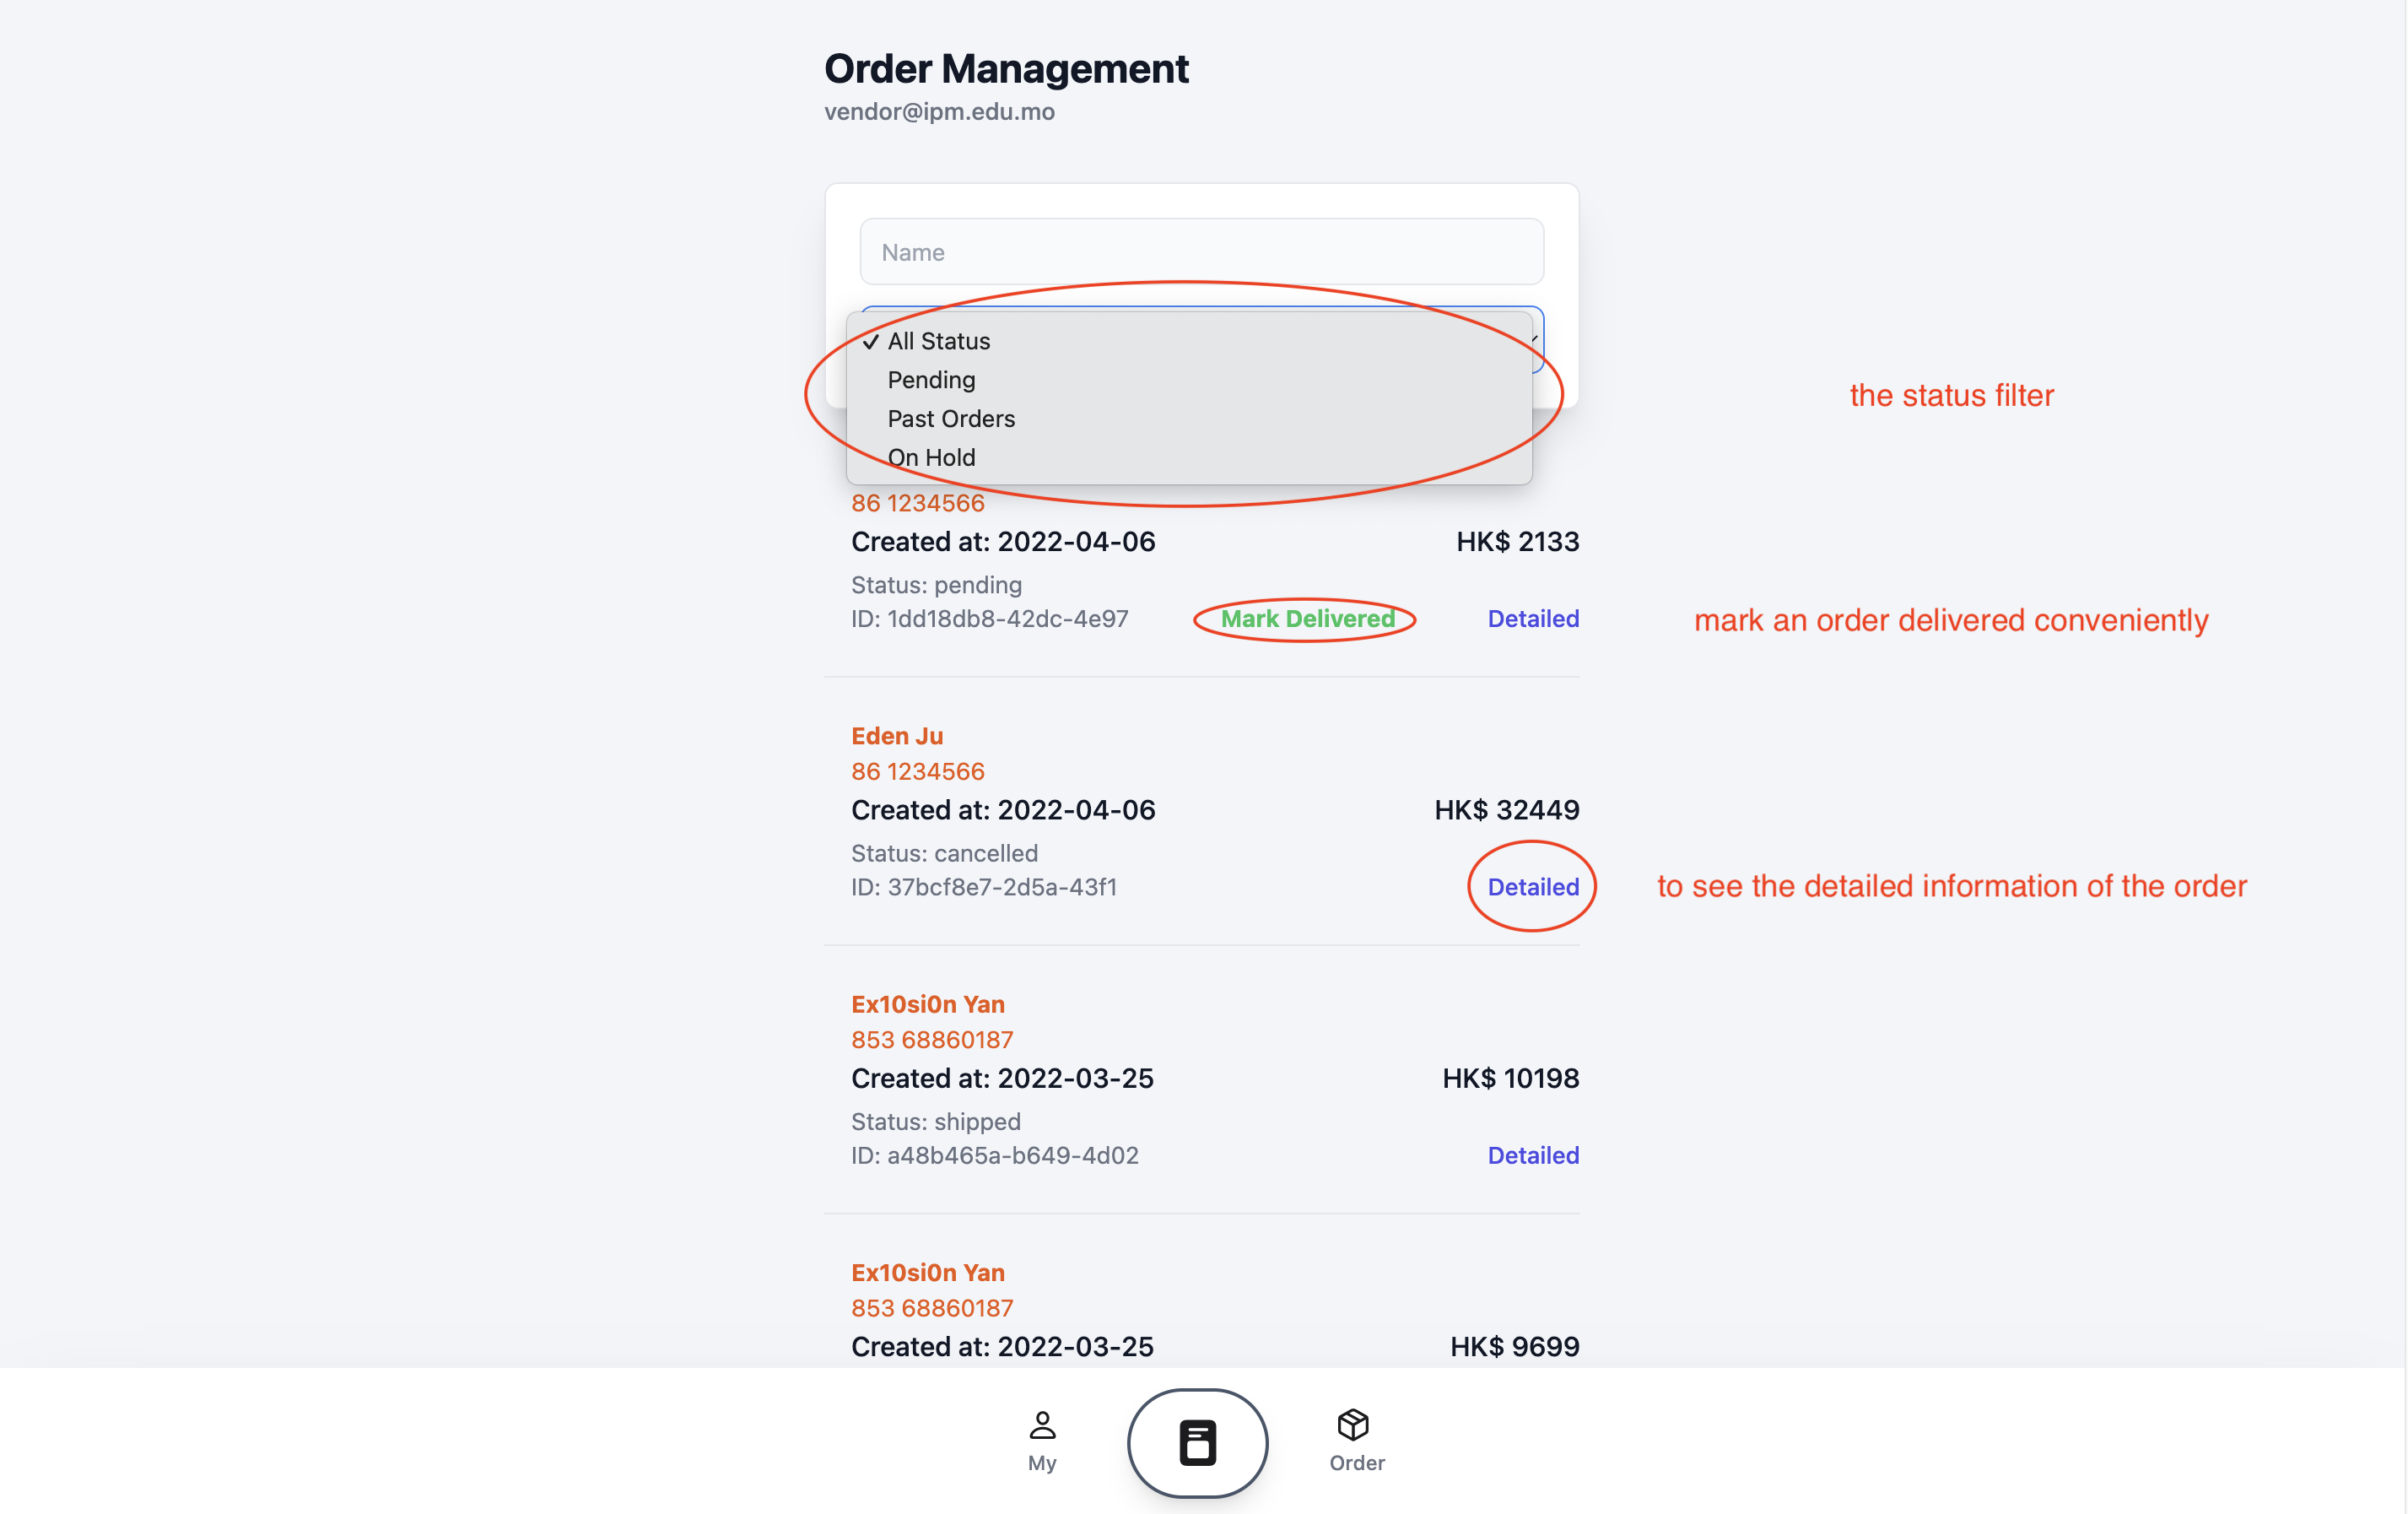
\includegraphics[width=0.72\textwidth]{order management.png}
    \caption{\label{fig:order management}The order management page}
\end{figure}
\\\\
The vendor can mark an order as delivered conveniently in the column and the detail button guides the vendor to view any further detailed order information such as the names and quantity of all the purchased products. In this purchase order processing page, the order status is highlighted in different color.
\\\\
When an order is in pending status, it can be delivered if it has been shipped successfully or be changed into "hold" if the product is temporarily out-of-stock. When the desired product of an order held by the vendor is in stock, it can then be delivered.
\begin{figure}[htbp]
\centering
\begin{minipage}[t]{0.48\textwidth}
\centering
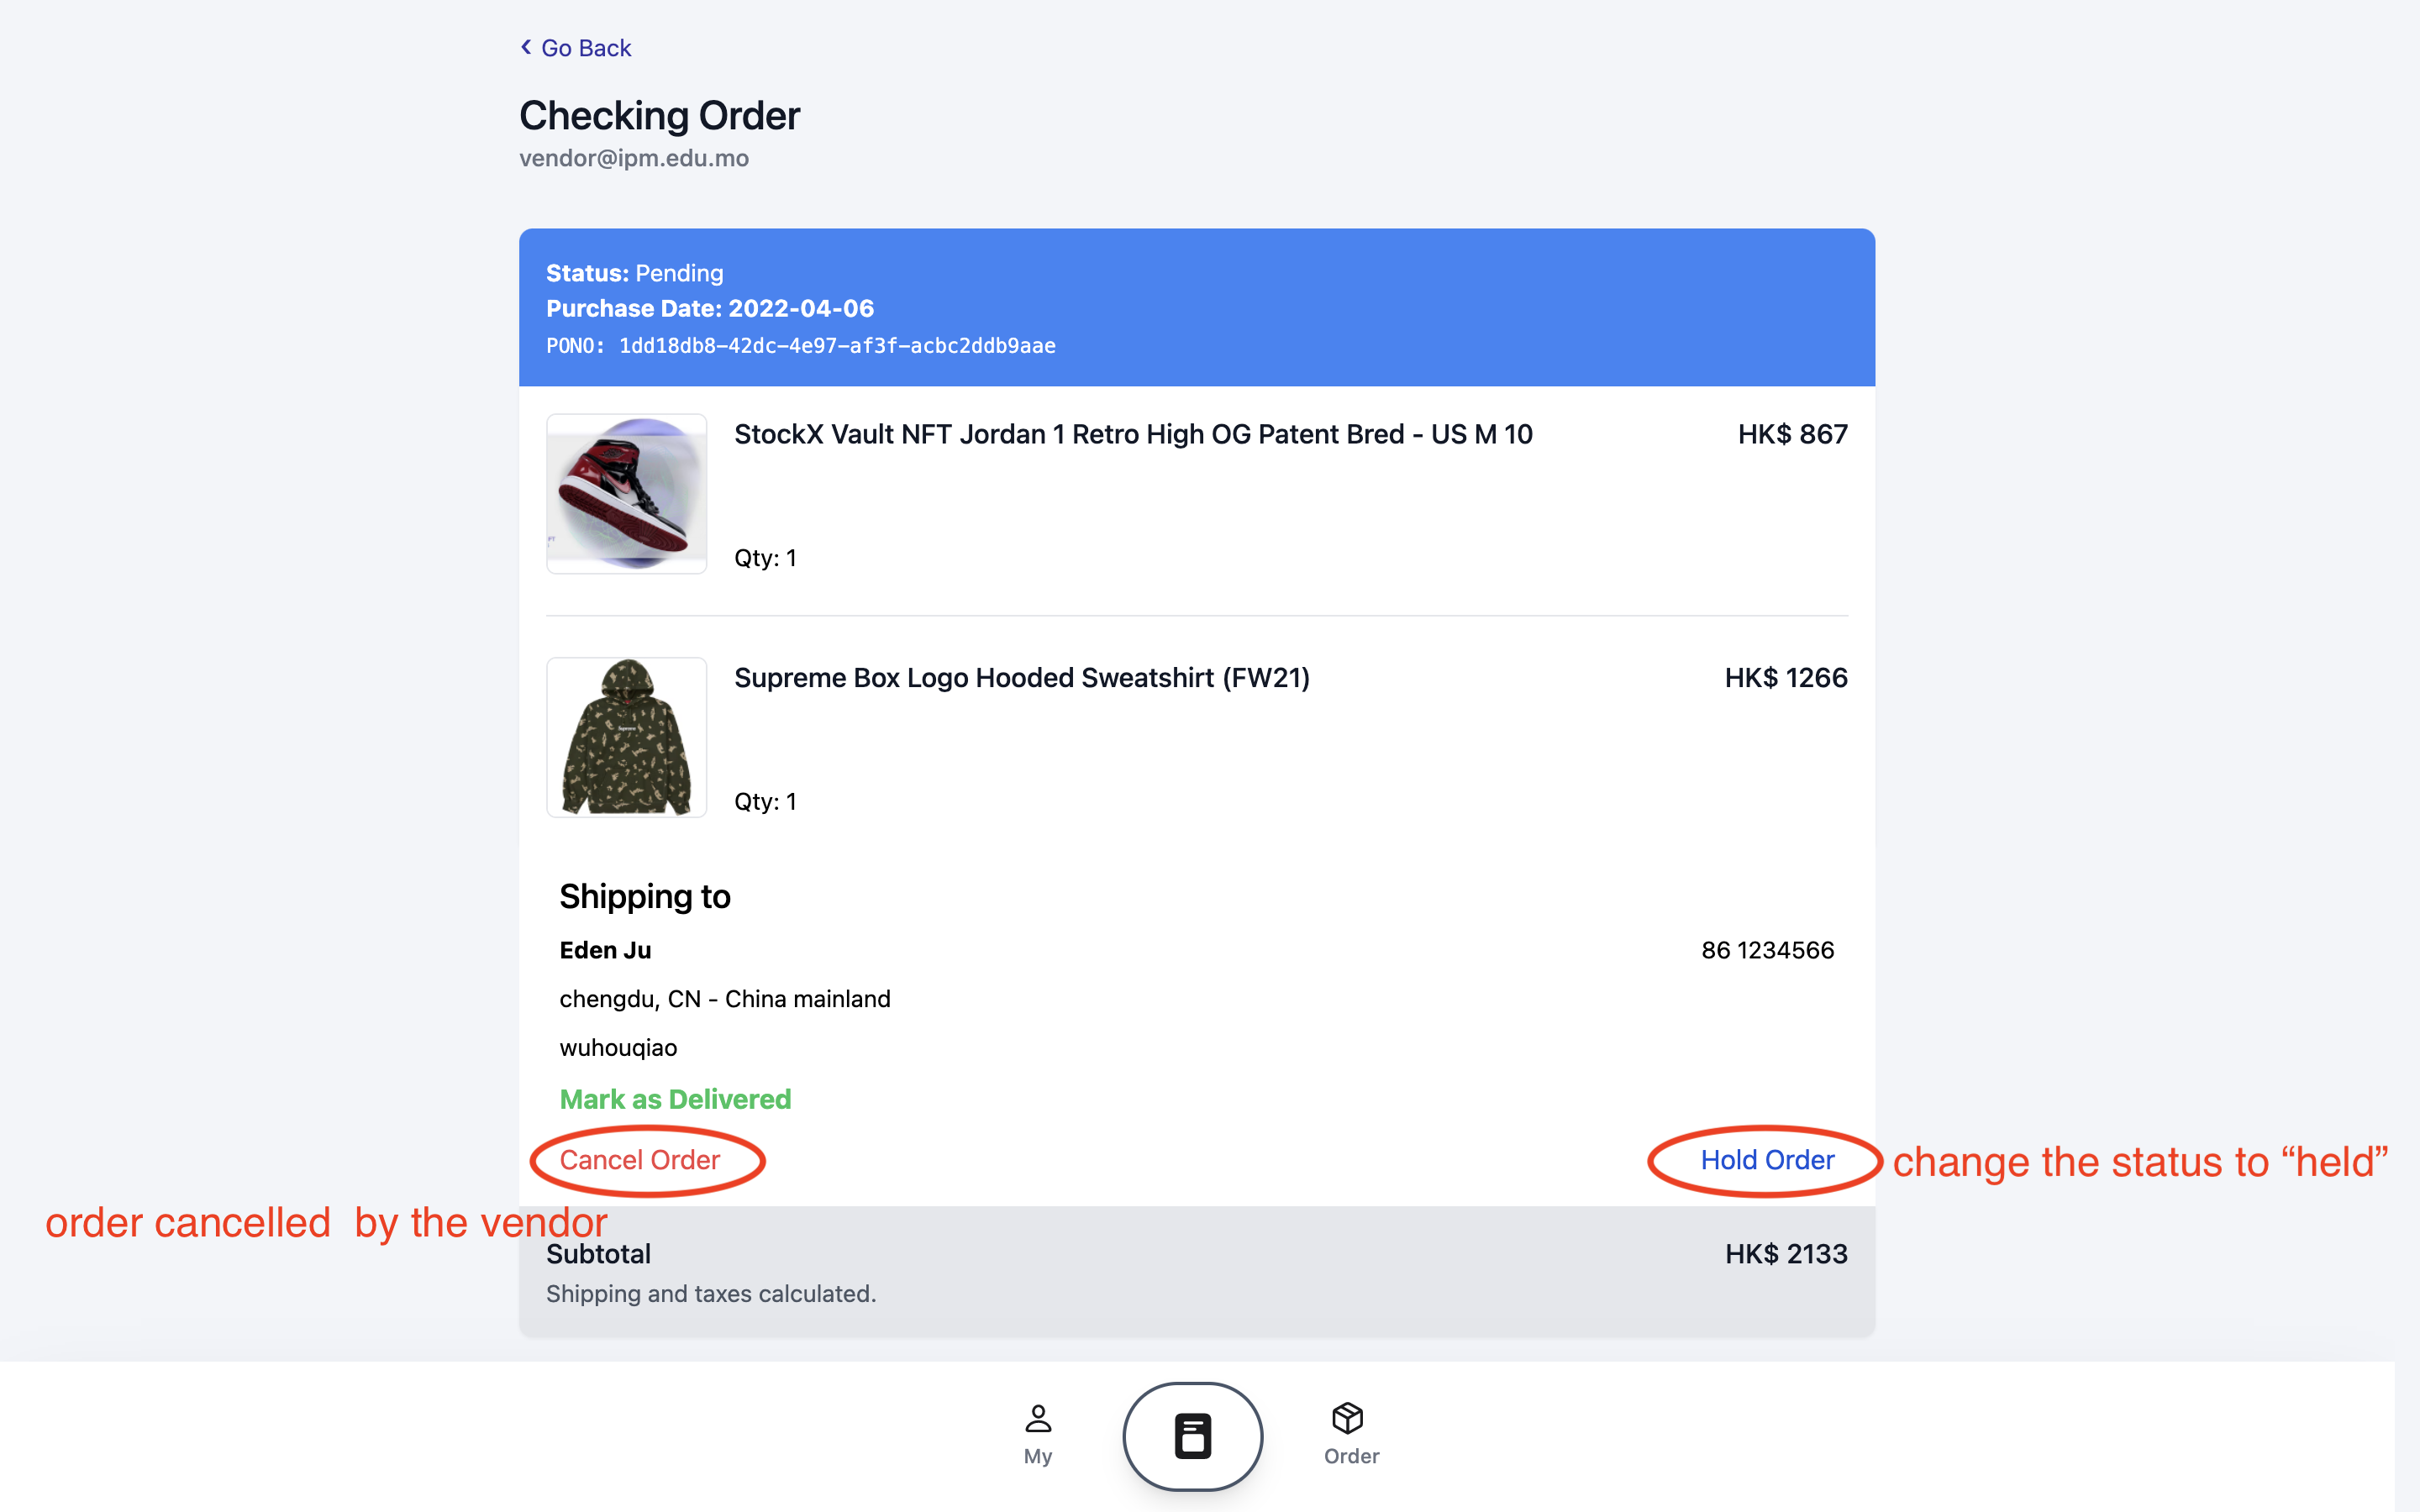
\includegraphics[width=6cm]{pending.png}
\caption{A pending order}
\end{minipage}
\begin{minipage}[t]{0.48\textwidth}
\centering
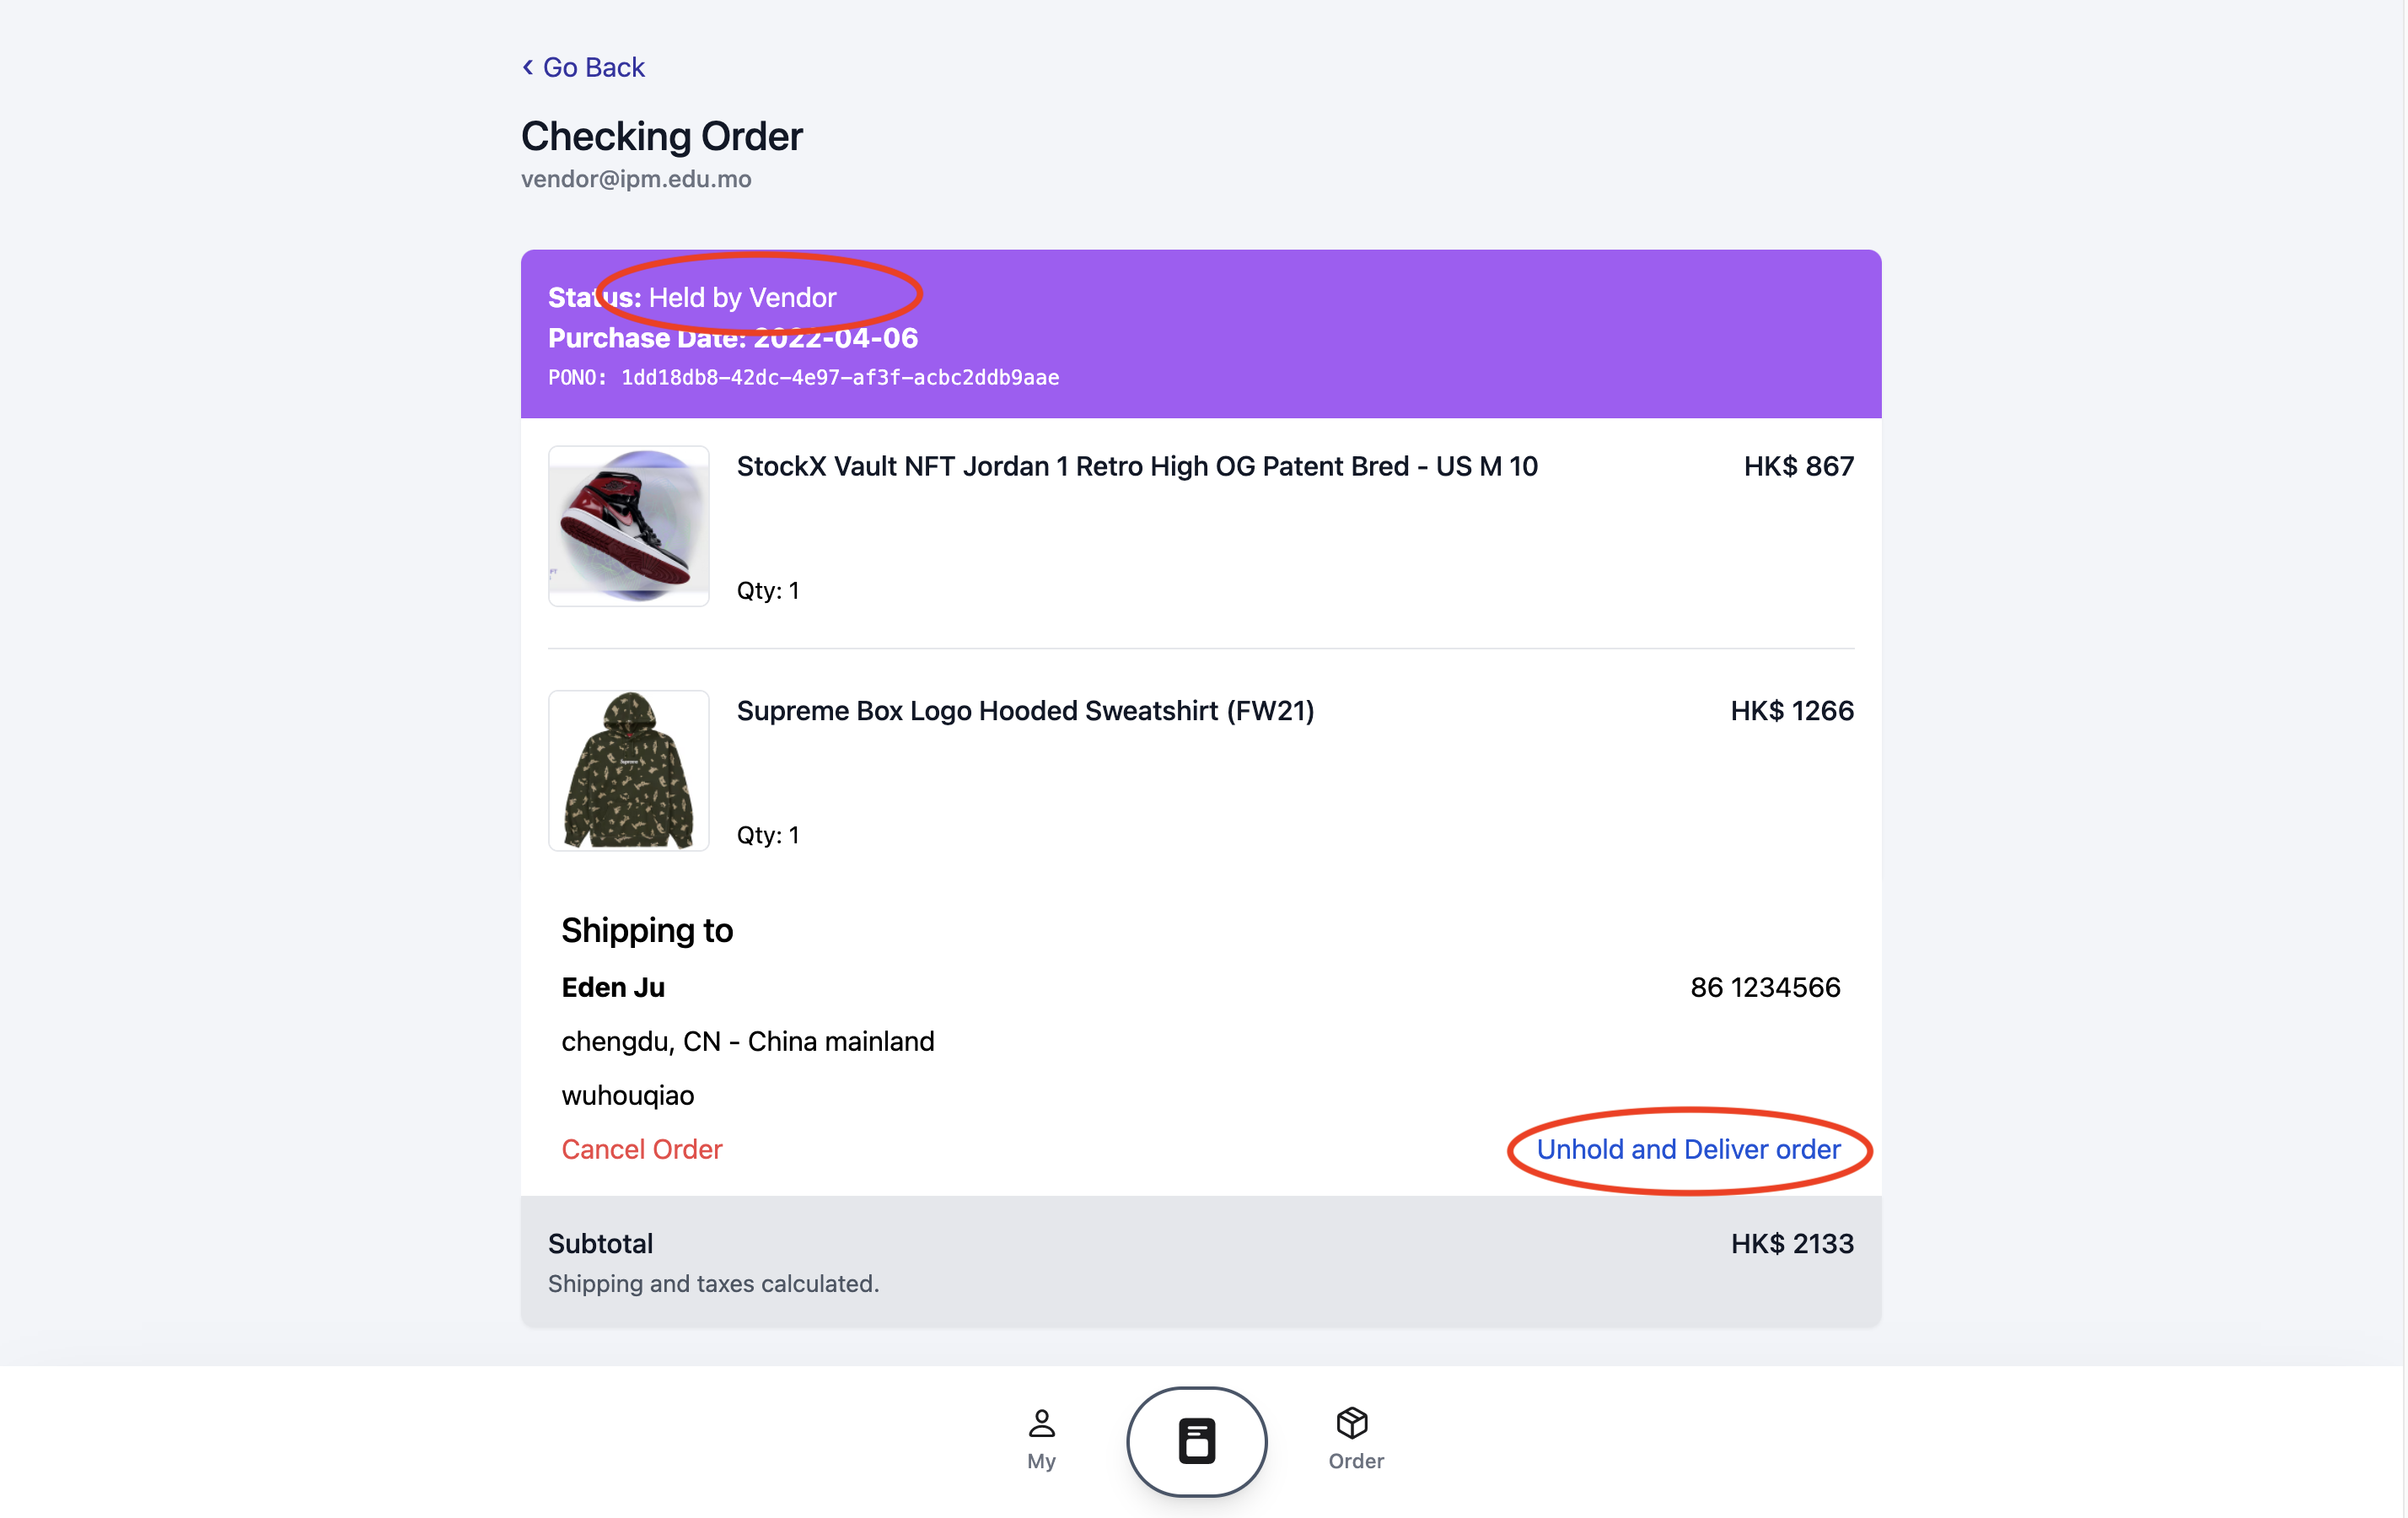
\includegraphics[width=6cm]{held by vendor.png}
\caption{An order held by the vendor}
\end{minipage}
\end{figure}
\\\\
Each order that has not been shipped can be marked as cancelled either by the user or the vendor. The person who cancels this order will also be recorded in this order detailed page.
\begin{figure}[htbp]
\centering
\begin{minipage}[t]{0.48\textwidth}
\centering
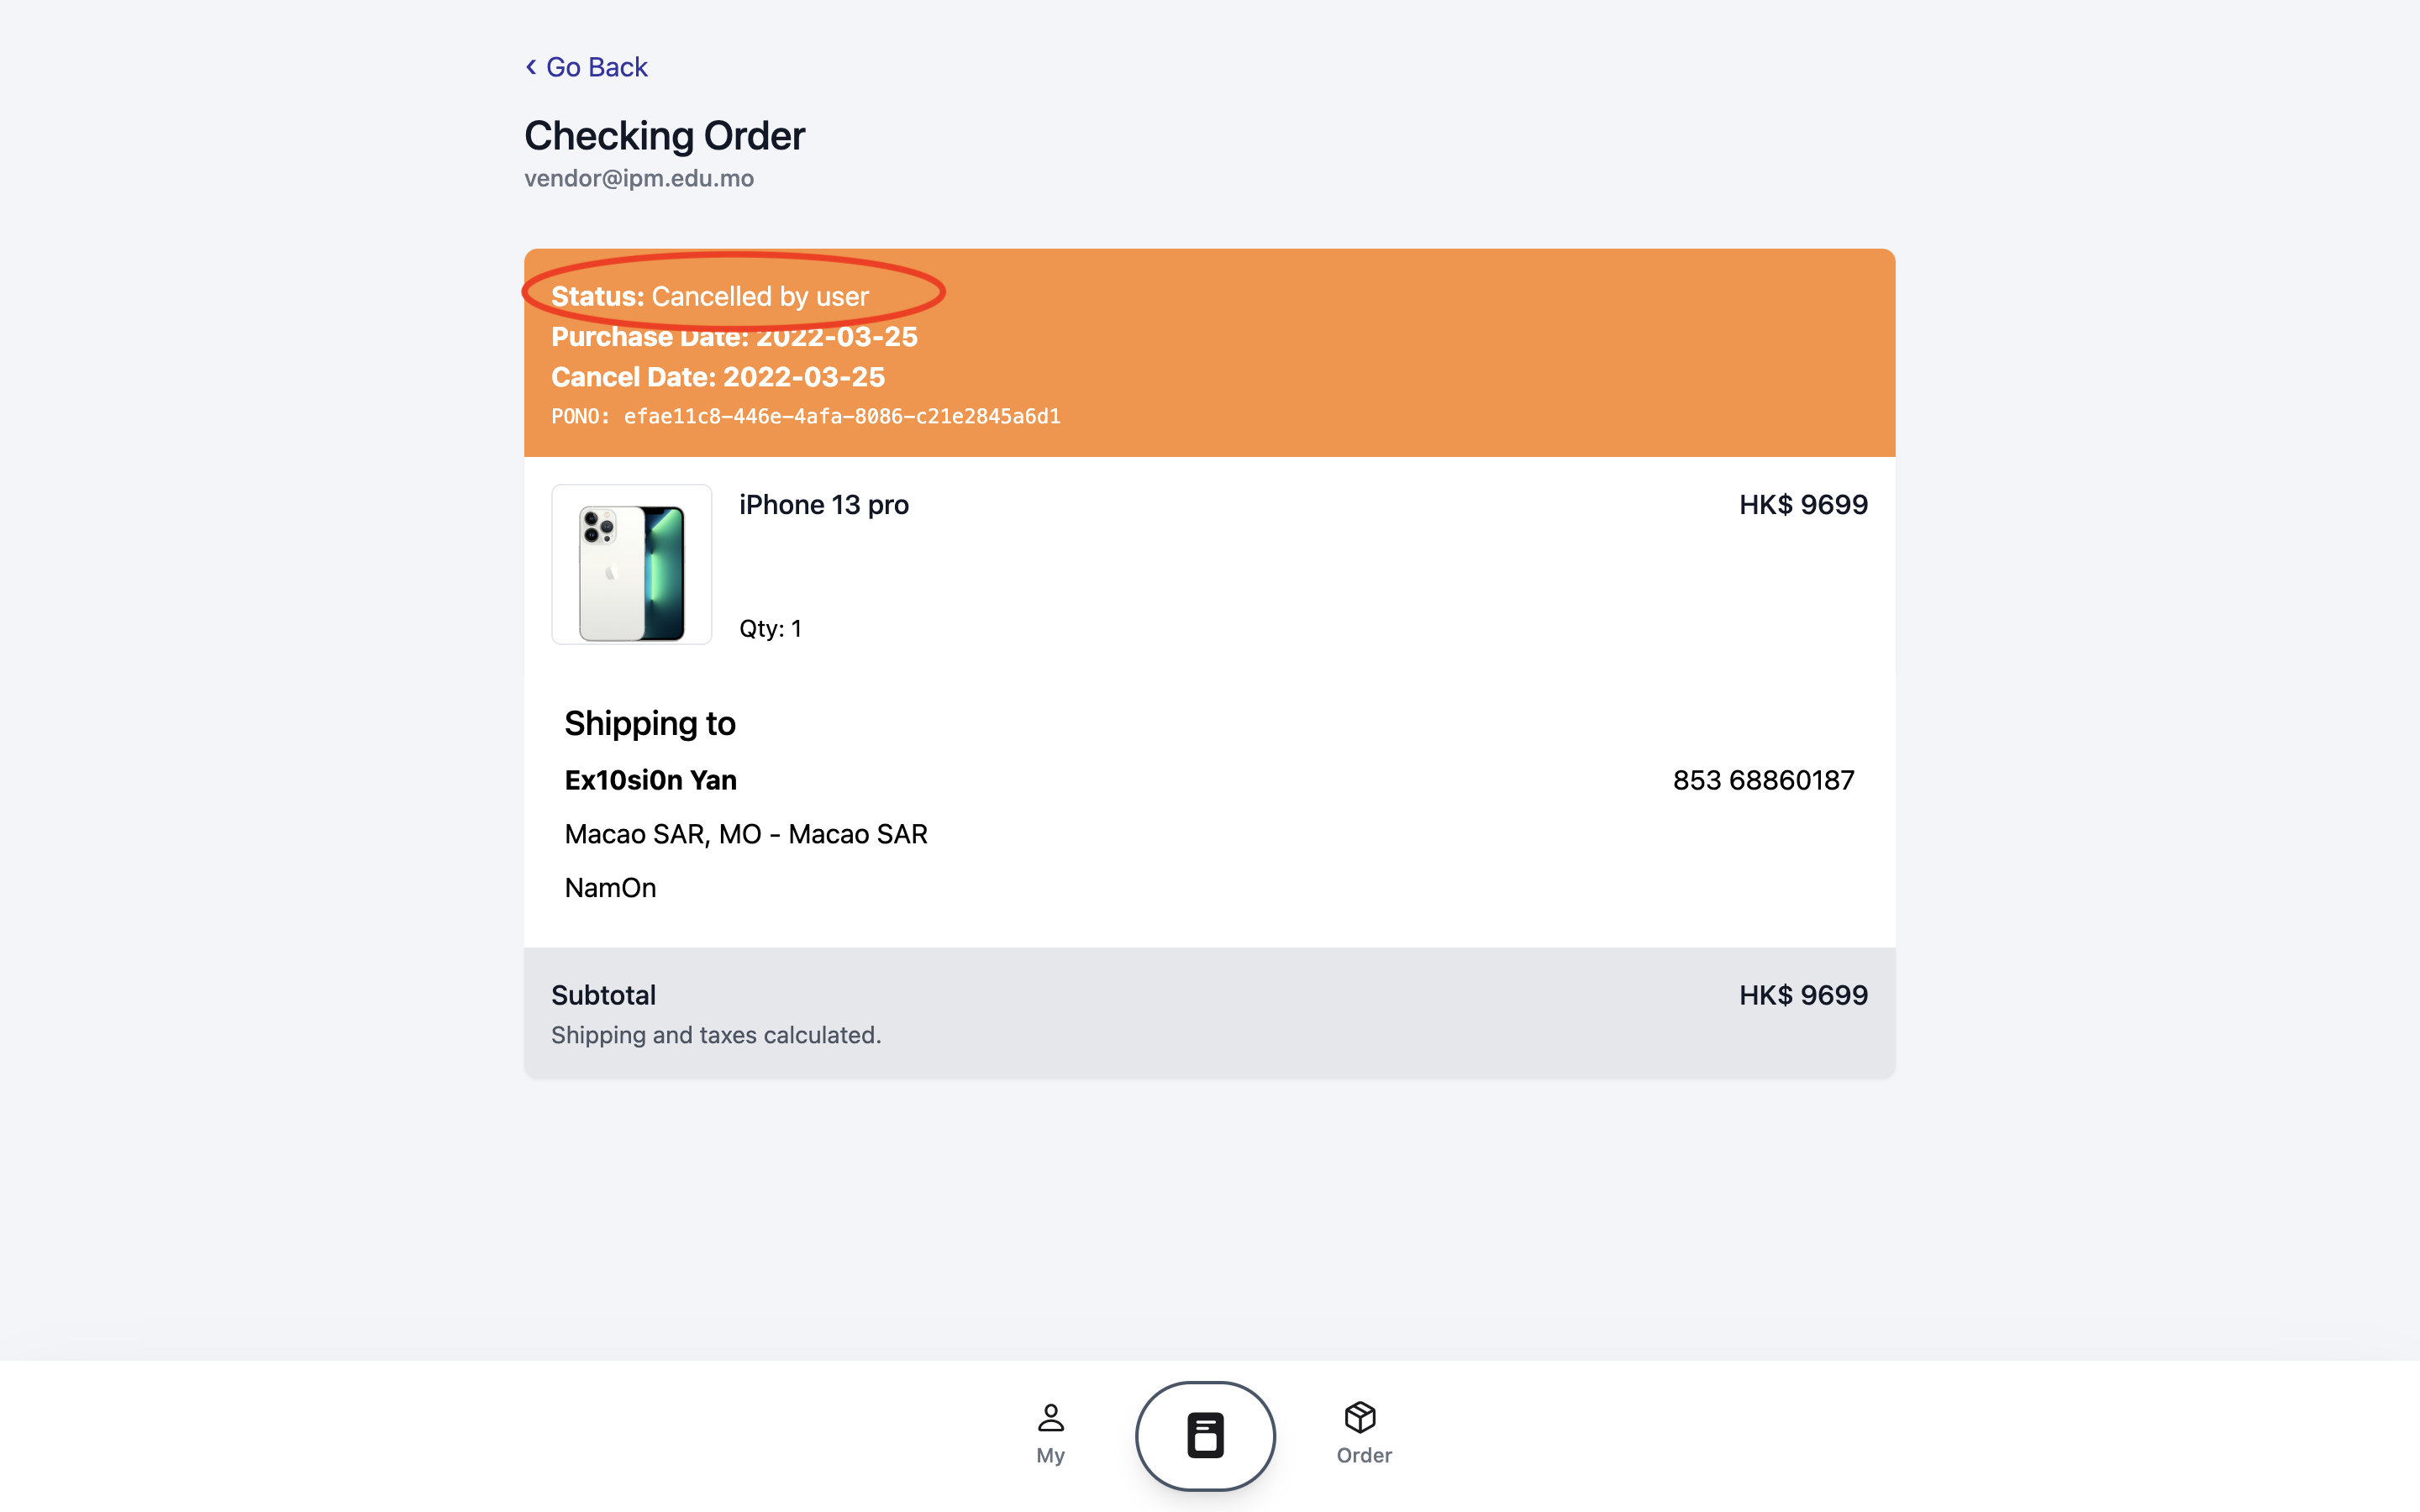
\includegraphics[width=6cm]{cancelled by user.png}
\caption{An order cancelled by the user}
\end{minipage}
\begin{minipage}[t]{0.48\textwidth}
\centering
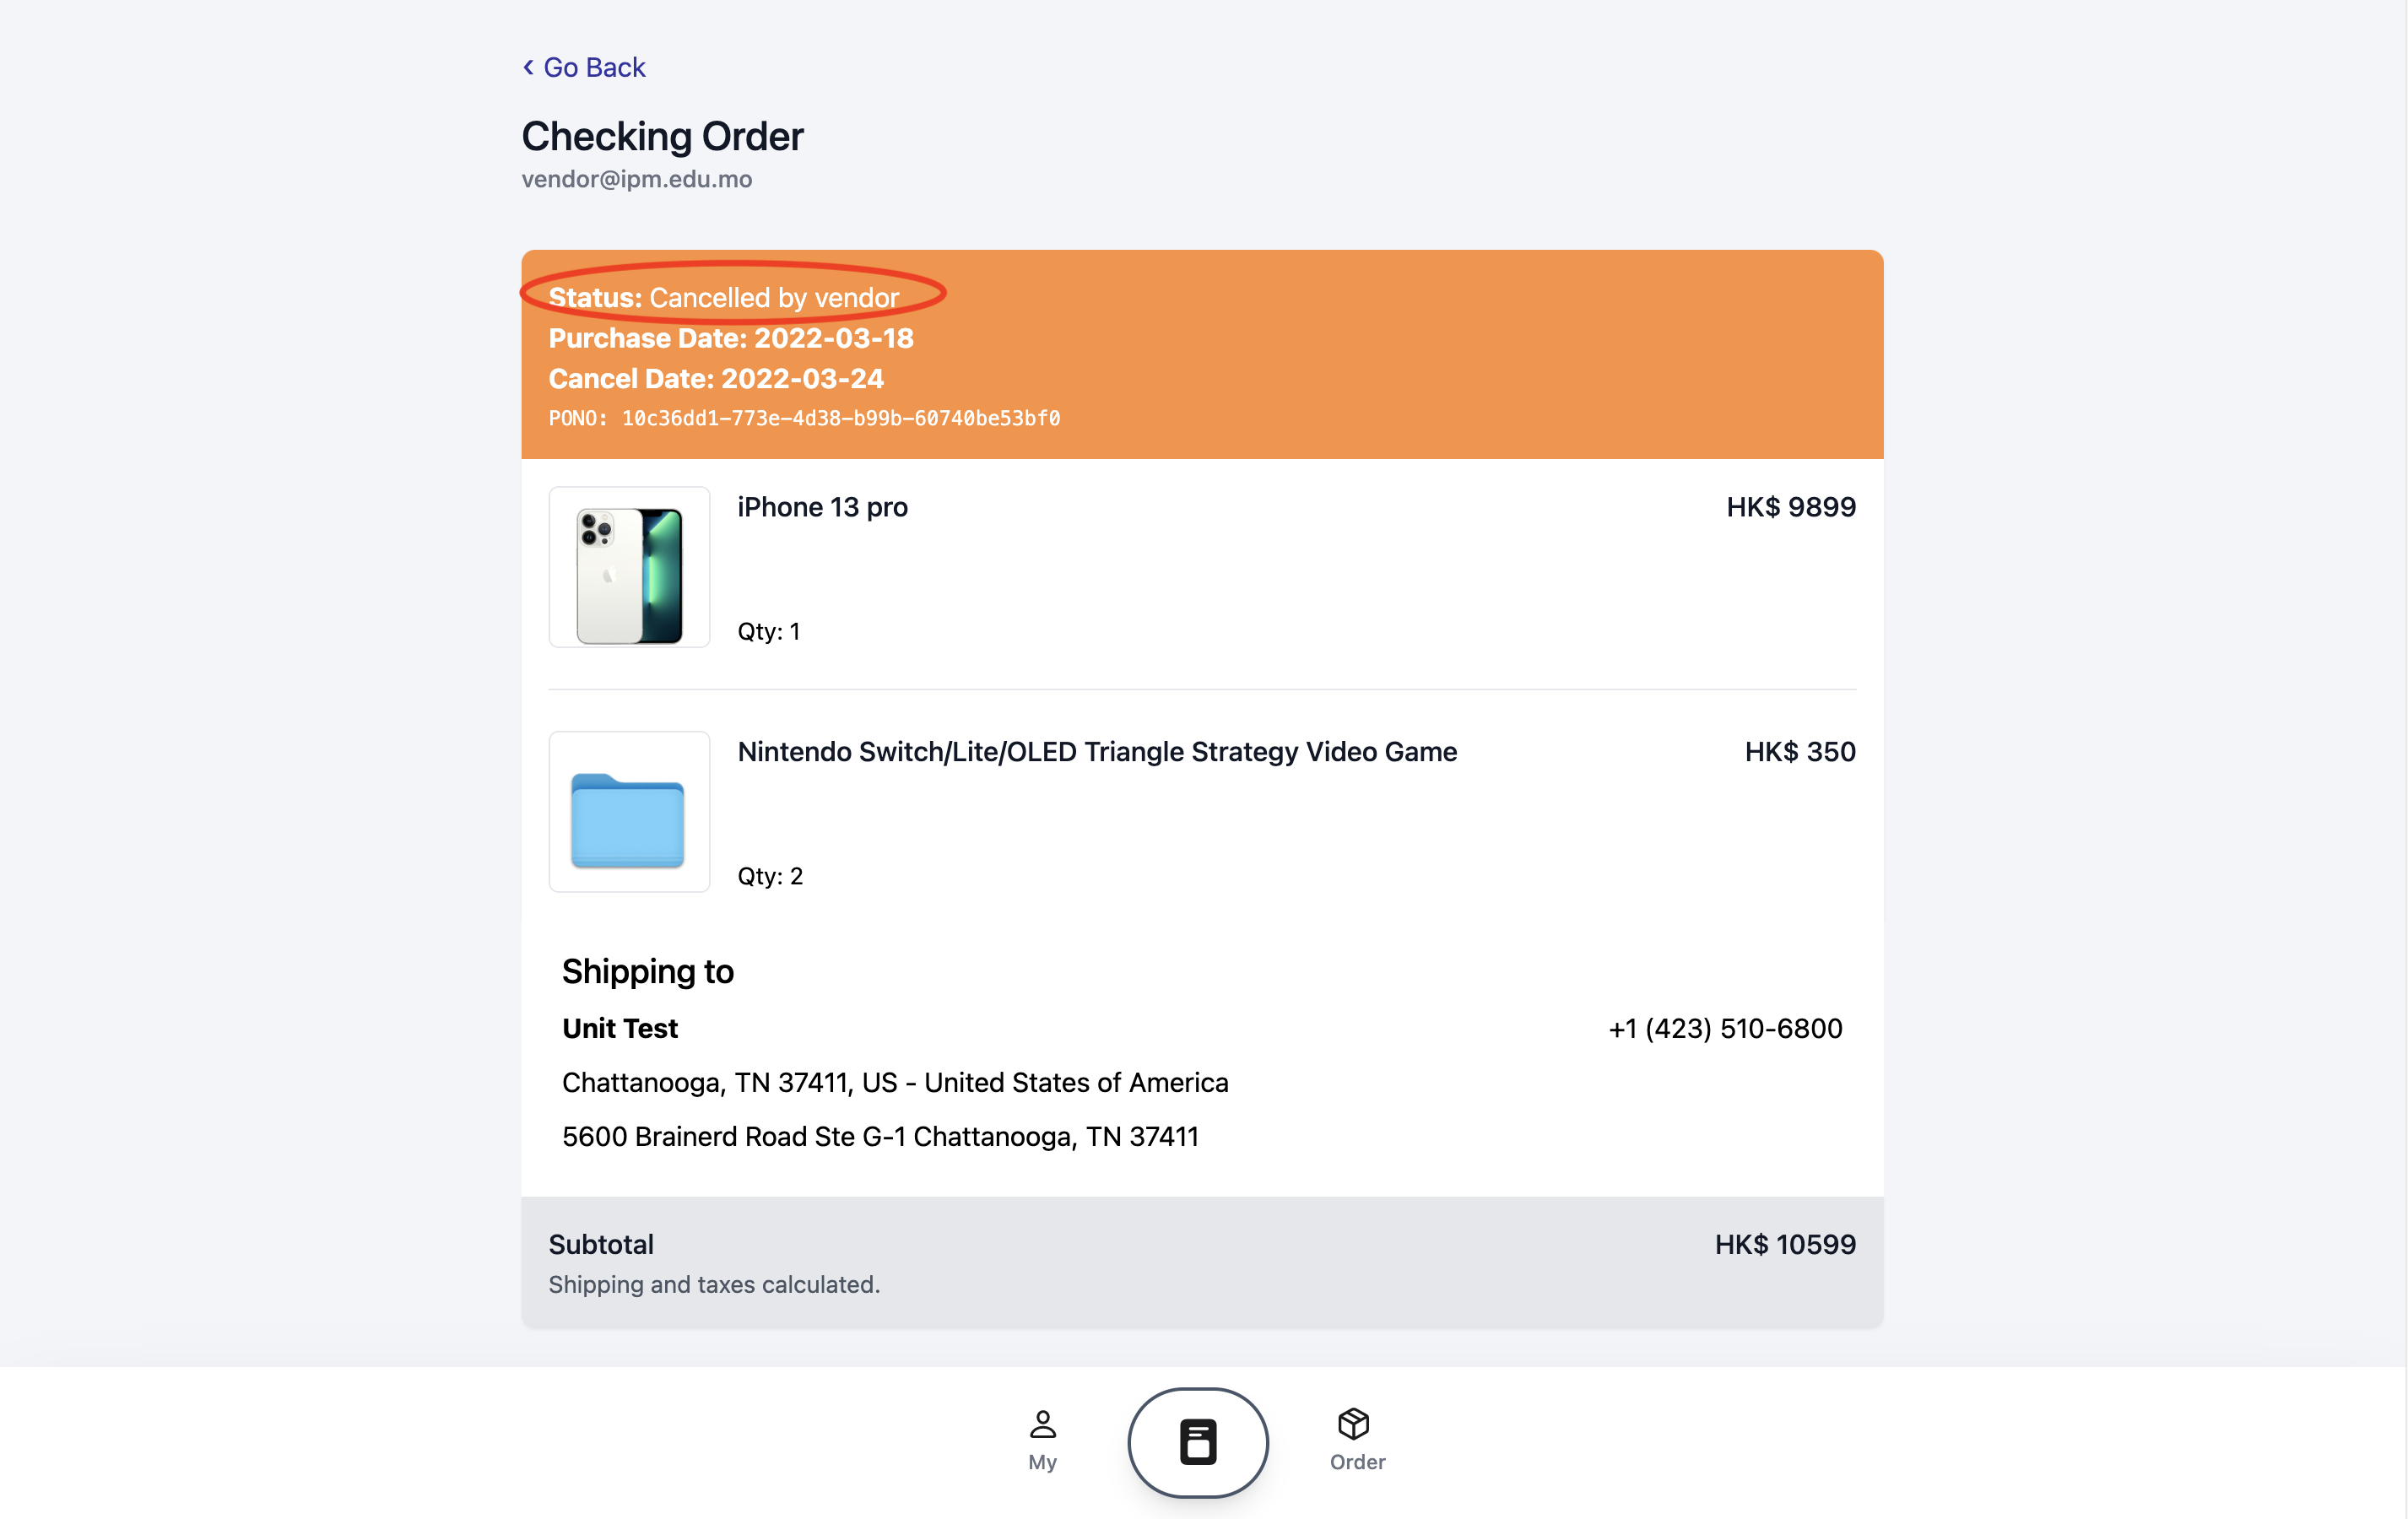
\includegraphics[width=6cm]{cancelled by vendor.png}
\caption{An order cancelled by the vendor}
\end{minipage}
\end{figure}
\\\\
Finally, it will also record the shipment date if an order is shipped successfully.
\begin{figure}[!htp]
    \centering
    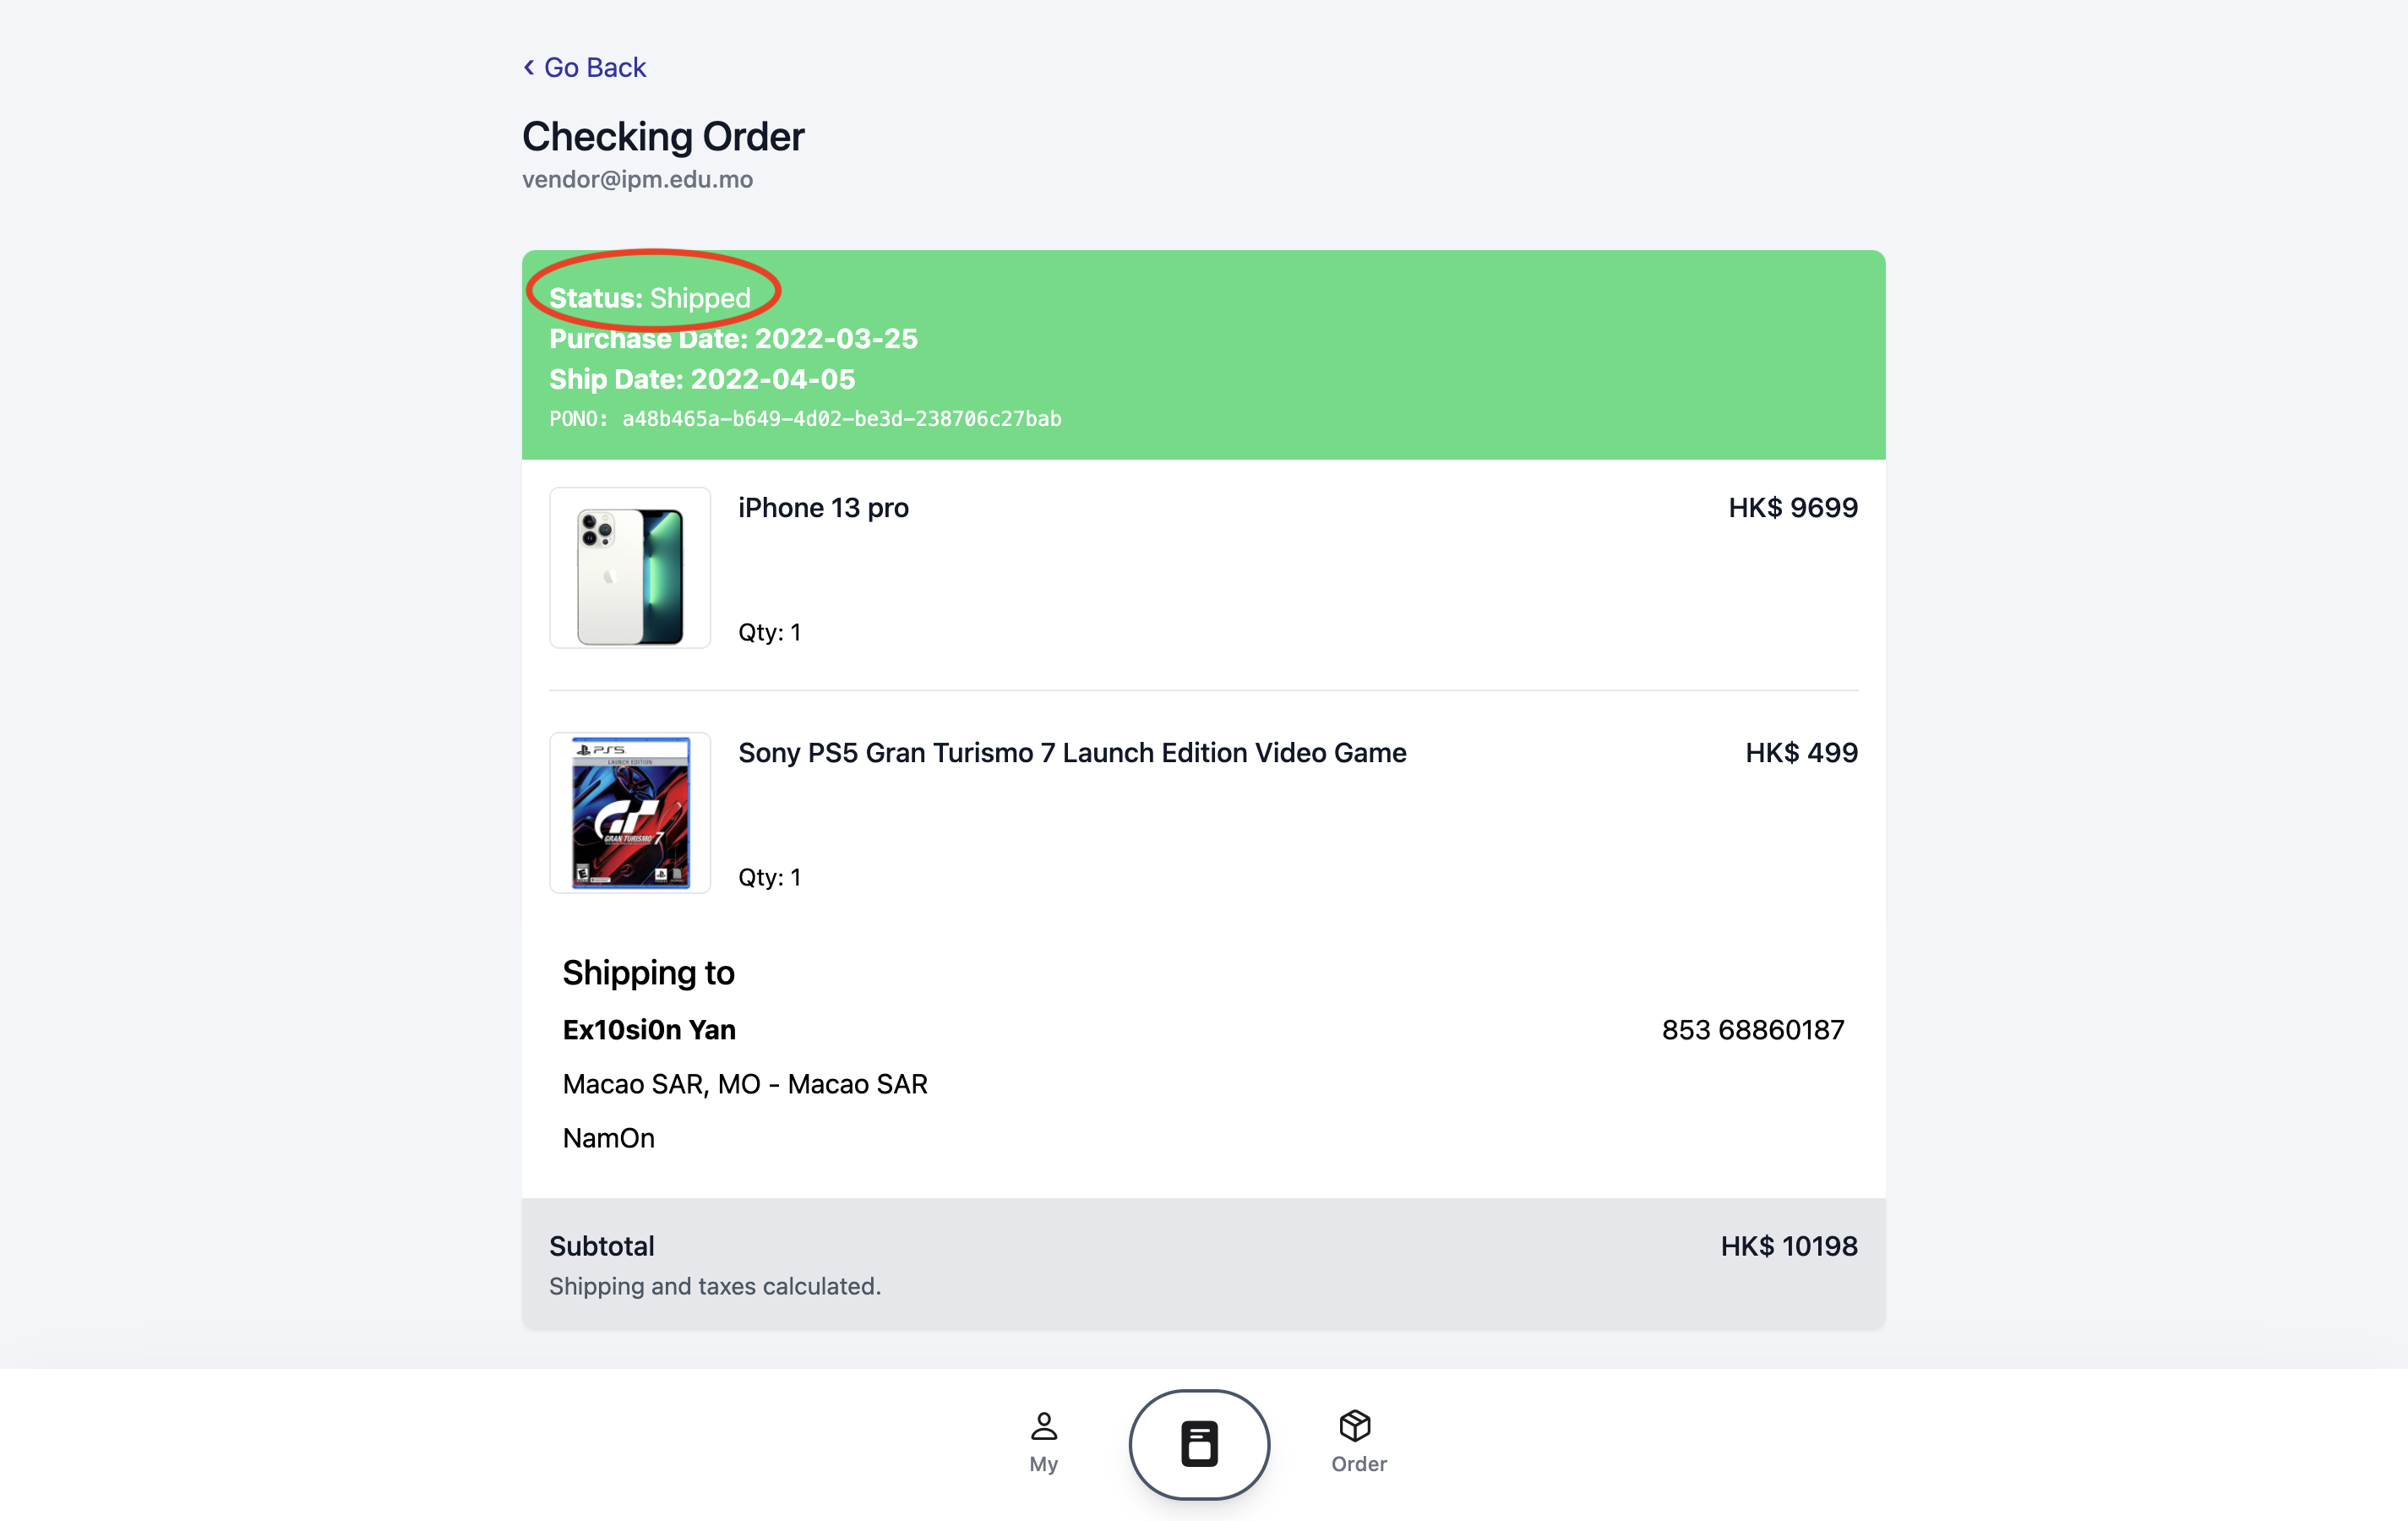
\includegraphics[width=0.48\textwidth]{shipped.png}
    \caption{\label{fig:shipped}A shipped order}
\end{figure}

\subsubsection{Mobile Application}

A hybrid IOS software of the OpenMall project has been developed for Apple users. [see Figure \ref{fig:mobile desktop}] 
\begin{figure}[!htp]
    \centering
    
\includegraphics[width=0.2\textwidth]{desktop.jpg}
    \caption{\label{fig:mobile desktop} application icon on the mobile desktop }
\end{figure}
\\\\
The mobile application can communicate with the server backend through a Web API as the web application. Moreover, the UI layouts are consistent with the UI layouts in the web application. The consistency between the mobile application and the web application is in order to reduce the learning cost of users to use the mobile application. 	
\\\\
Then the following screen captures briefly shown our mobile application. 	
\\\\
Customer:
\begin{figure}[htbp]
\centering
\subfigure[Customer order detail]{
\begin{minipage}[t]{0.25\linewidth}
\centering
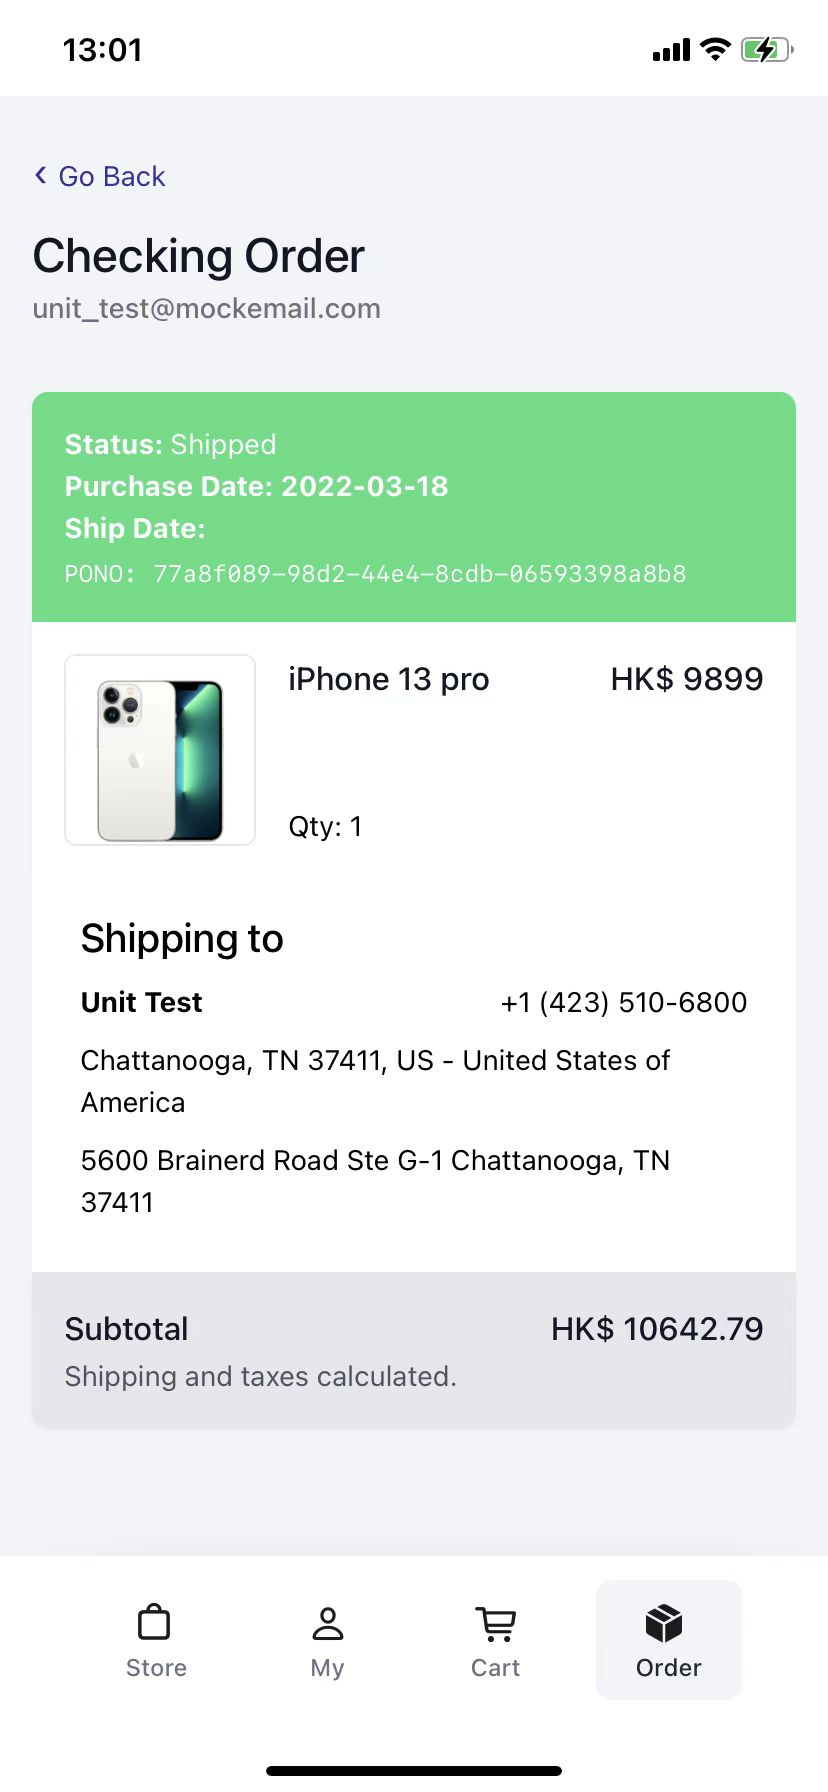
\includegraphics[width=1in]{app order detail.jpg}
%\caption{fig1}
\end{minipage}%
}%
\subfigure[Customer product detail]{
\begin{minipage}[t]{0.25\linewidth}
\centering
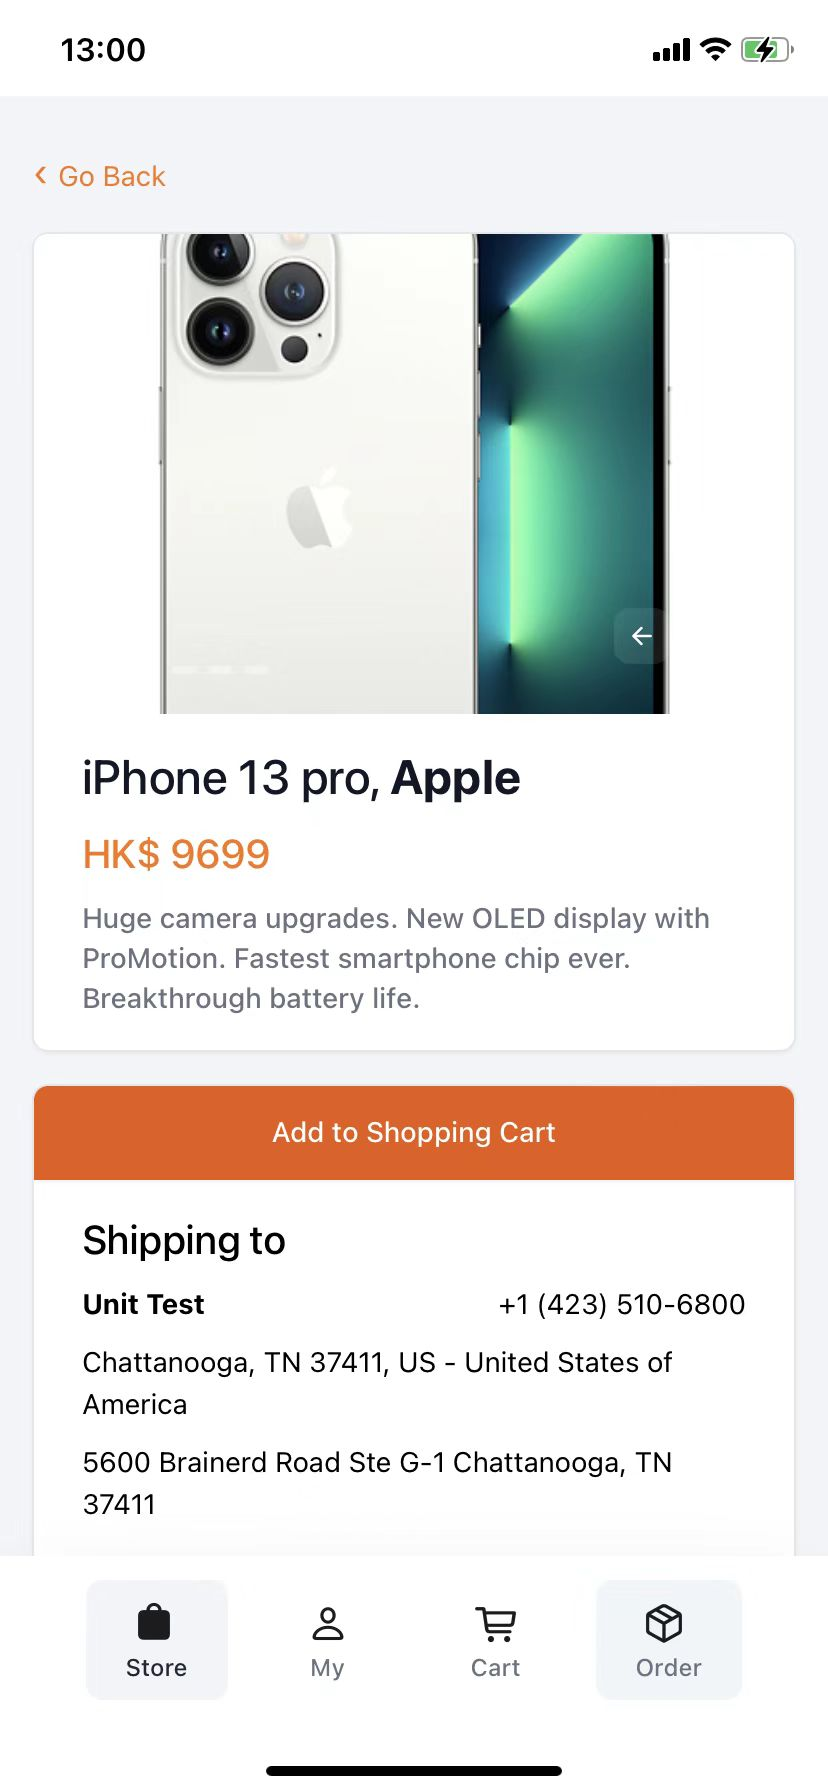
\includegraphics[width=1in]{app product detail.jpg}
%\caption{fig2}
\end{minipage}%
}%
\subfigure[Customer product list]{
\begin{minipage}[t]{0.25\linewidth}
\centering
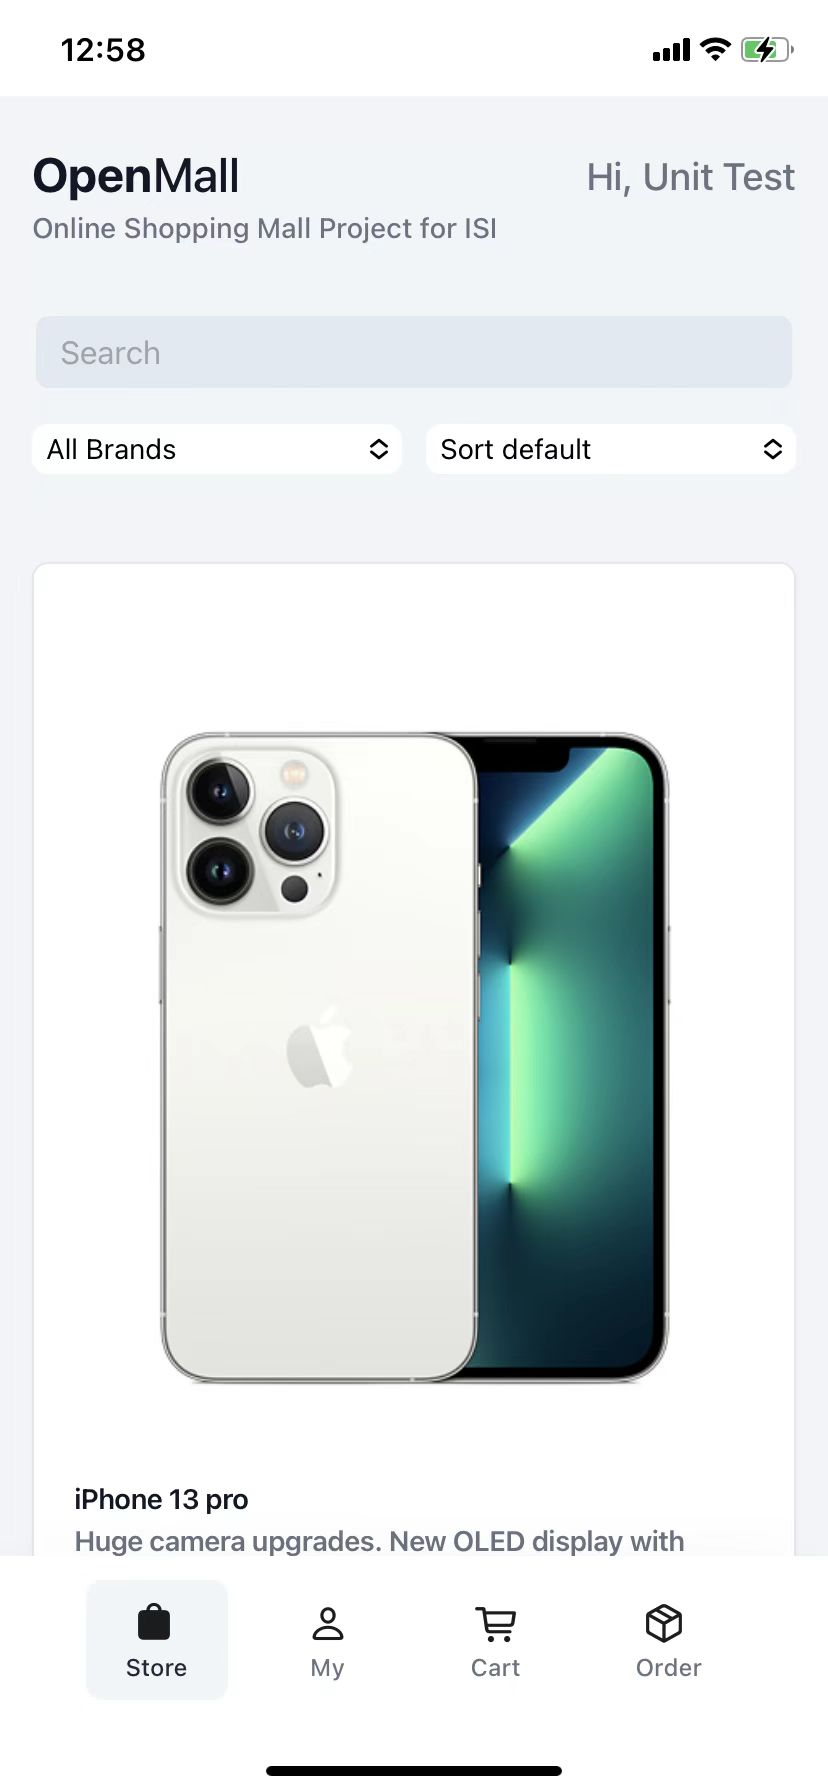
\includegraphics[width=1in]{app product list.jpg}
%\caption{fig2}
\end{minipage}
}%
\subfigure[Customer shopping cart]{
\begin{minipage}[t]{0.25\linewidth}
\centering
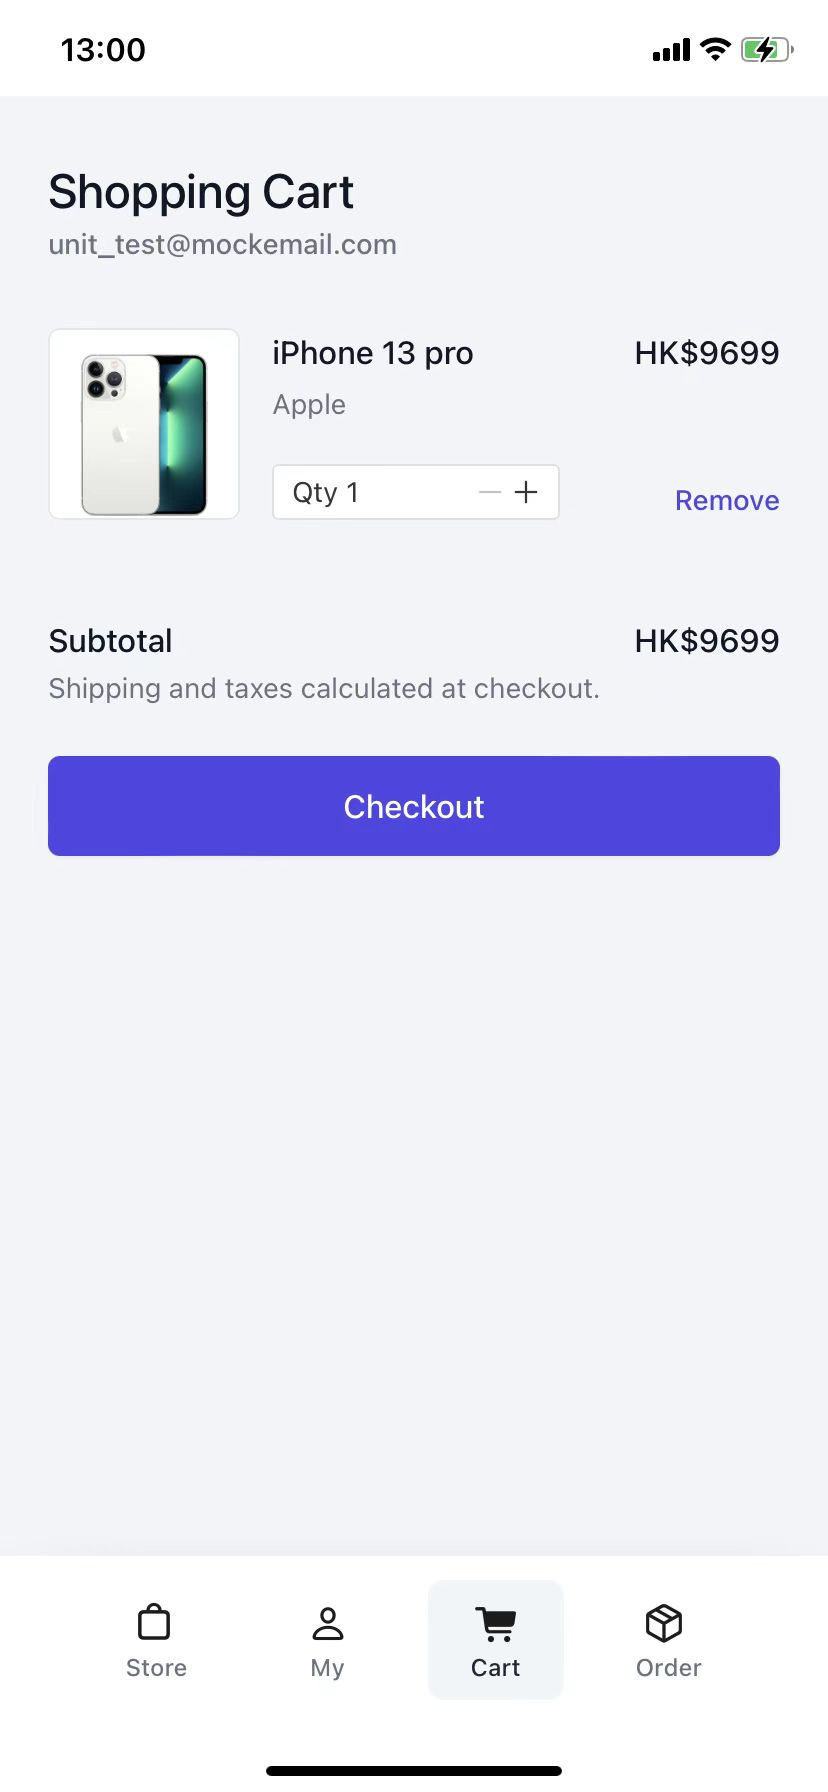
\includegraphics[width=1in]{app shopping cart.jpg}
%\caption{fig2}
\end{minipage}
}%
\centering
\caption{Customer view}
\end{figure}
\leavevmode
\\\\
Vendor:
\begin{figure}[htbp]
\centering
\subfigure[Vendor dashboard]{
\begin{minipage}[t]{0.25\linewidth}
\centering
\includegraphics[width=1in]{app vendor dashboard.jpg}
%\caption{fig1}
\end{minipage}%
}%
\subfigure[Vendor order detail]{
\begin{minipage}[t]{0.25\linewidth}
\centering
\includegraphics[width=1in]{app vendor order detail.jpg}
%\caption{fig2}
\end{minipage}%
}%
\subfigure[Vendor order list]{
\begin{minipage}[t]{0.25\linewidth}
\centering
\includegraphics[width=1in]{app vendor order management.jpg}
%\caption{fig2}
\end{minipage}
}%
\subfigure[Vendor update product]{
\begin{minipage}[t]{0.25\linewidth}
\centering
\includegraphics[width=1in]{app update product.jpg}
%\caption{fig2}
\end{minipage}
}%
\centering
\caption{Vendor view}
\end{figure}

\subsection{Testing and System Evaluation}

\subsubsection{Test Case}
 
 For test case, we have used Boundary Value Analysis, State Transition Techniques and Error Guessing Technique to design the test cases. Moreover, a requirements traceability matrix with test cases and test results were created as the requirements traceability matrix table shown below. After testing, the OpenMall project has passed all the test cases and has met all the feature requirements.
 \newpage
 
 matrix
 \newpage

\subsubsection{Robustness testing against SQL injection}

SQL injection is a code injection technique that might destroy the database. SQL injection is one of the most common web hacking techniques. SQL injection is the placement of malicious code in SQL statements via web page input.
\\\\
The Model to handle the database interaction is \verb|src/database.py|. We import a Python module \verb|PyMySql| as the database connector. And the cursor of the database connector fetches and updates data in the database. A sample cursor is shown as the code \ref{listing:cursor}.
\\\\
The SQL statement for checking a particular user from the database is \ref{listing:sql}

\begin{listing}[!htp]
\begin{minted}{sql}
SELECT * 
FROM `account` 
WHERE `email`=%s;
\end{minted}
\caption{Partial SQL for login check}
\label{listing:sql}
\end{listing}

To apply the SQL injection method, we can construct a malicious
string by adding an extra logic operator to pass the gate of the E-mail checker. The constructed SQL command is \ref{listing:constructedSQL}.
\begin{listing}[!htp]
\begin{minted}{sql}
SELECT * 
FROM `account` 
WHERE `email`='no-email' or 1 = 1; --';
\end{minted}
\caption{Constructed SQL}
\label{listing:constructedSQL}
\end{listing}

Due to the \verb|%s| in the checker gate SQL, Python will add a pair of apostrophes surrounding the user E-mail. Then we construct a string containing a close apostrophe after \verb|no-email| and use \verb|--| to comment out the ending apostrophe generated by the Python string. [see \ref{fig:sql-inj}] Then for the malicious string \ref{listing:maliciousString}, it should cancel the E-mail checker gate and let the model return a response rather than the \verb|account_not_registered|.

\begin{listing}[!htp]
\begin{minted}{python}
no-email' or 1 = 1; --
\end{minted}
\caption{The malicious string for SQL injection}
\label{listing:maliciousString}
\end{listing}

\begin{figure}[!htp]
    \centering
    \includegraphics[width=0.6\textwidth]{sql-inj.png}
    \caption{\label{fig:sql-inj}Failure applied of SQL injection}
\end{figure}

However, with the protection by the parameterized statement provided by \verb|PyMySql|, the SQL injection could not be applied. 
\begin{listing}[!htp]
\begin{minted}{python}
with connection:
    with connection.cursor() as cursor:
        sql = "SELECT * FROM `account` WHERE `email`=%s"
        cursor.execute(sql, (email,))
        result = cursor.fetchone()
        if (result is None):
            playload['status'] = 'account_not_registered'
            return playload
        given_hashed_password = password_validator.hash(
            password, result['ACCID'])
        # Accept the user with correct password
        if given_hashed_password == result['HASHEDPASSWORD']:
            playload['status'] = 'success'
            playload['uuid'] = result['ACCID']
            playload['type'] = result['ACCTYPE']
            return playload
        else:
            playload['status'] = 'invalid_password'
            return playload
\end{minted}
\caption{Database cursor}
\label{listing:cursor}
\end{listing}

\subsubsection{Robustness testing against XSS Attack}

Cross-Site Scripting (XSS) attacks are a type of injection, in which malicious scripts are injected into otherwise benign and trusted websites. XSS attacks occur when an attacker uses a web application to send malicious code, generally in the form of a browser side script, to a different end user. Flaws that allow these attacks to succeed are quite widespread and occur anywhere a web application uses input from a user within the output it generates without validating or encoding it. \cite{xss}
\\\\
\begin{figure}[htbp]
\centering
\begin{minipage}[t]{0.48\textwidth}
\centering
\includegraphics[width=6cm]{xss.png}
\caption{\label{fig:xss}Cross site scripting Attack}
\end{minipage}
\begin{minipage}[t]{0.48\textwidth}
\centering
\includegraphics[width=6cm]{xss-outcome.png}
\caption{\label{fig:xss-outcome}The outcome of XSS attack}
\end{minipage}
\end{figure}
\\\\
Dangerous characters like \verb|>| and \verb|<| are escaped by changing to \verb|&gt| and \verb|&lt|. That's because of Vue.js' template rendering. OpenMall adopts the method of separating the front and back ends and encapsulates the data in JSON. Data is transmitted and received by the API, and Vue.js renders it as an HTML presentation. During rendering, it prevents data from dangerous characters.

\clearpage

\section{Conclusion and Further Work}
In this project, the Open Mall application with products browsing and maintenance, purchase orders and placing for multitype of users has been successfully implemented. Vue.js was used to build the front-end view and we implement the back-end API based on FastAPI. MariaDB was our database management system to build and maintain our database. Finally, Xcode SDK was used to port the web mall to a mobile application.
\\\\
For the front-end interfaces for users, the user login page,  product list page, product detail page, shopping cart page, purchase tracking page, and purchase order detail page have been designed for customers. Meanwhile, the product catalog maintenance page and purchase order list page have been built for vendors. All the front-end layout and style designs of pages were based on HTML5 and Tailwind CSS. The front-end logic was implemented based on the Vue.js framework. We tested and verified the whole shopping process of users and the mall maintenance process of vendors by the method of the cognitive walkthrough after deployment.
\\\\
As for the back-end part, the APIs that handle front-end requests and invoke the required data of the database have been implemented. All the APIs were built by the Python-based FastAPI Framework. We used MariaDB to build the database and implement six entities: \verb|Account, Address, Product,| \verb|Shopping Cart, Purchase, Order|. Moreover, various SQL query statements and permissions of different users have been defined.
\\\\
When it comes to porting the Open Mall web to a mobile application, the front-end interfaces have been restructured by using the Xcode SDK to make them available for mobile devices. We adopted the mode of hybrid web application to implement the iOS App. Once the code is written, the application can run on all the Apple platforms in favor of the SwiftUI. 
\\\\
Inevitably, there are also limitations in the Open Mall project. First of all, Open Mall was a web application running on the web browser, but not a native application. Therefore, the response time of the application is slightly slower than that of the native applications such as page load time. Secondly, logistics systems and payment gateways have not been integrated into the Open Mall application. What is more, the user’s community which allows users to make comments about the particular product and view evaluations from other users have not been implemented. Besides, the language system does not support for multi-language for the moment. 
\\\\
In the future, the Open Mall application will be updated to a native application for higher efficiency and response speed. A brand-new user community that supports users’ comments and communication in the form of pictures, text, and videos will be implemented. Additionally, the logistics system, payment gateways, and multi-language system will be tightly integrated into the Open Mall application. 


\clearpage

\renewcommand\listoflistingscaption{List of source codes}

\bibliographystyle{IEEEtran}
\bibliography{reference}

\clearpage



\clearpage
\section{Appendix A: Project Management}
There are four parts– Project Scope Management, Project Time Management, Project Human Resource Management, Changes and Adjustments. Since this project does not involve the cost, Project Cost Management is omitted.
\begin{list}{\labelitemi}{\leftmargin=1em}
\item \subsection*{Project Scope Management}
\end{list}
Project scope management includes the processes involved in defining and controlling what is or is not included in a project. And for this project, all basic functions and the additional function Z0 are included. This chapter describes the Work Breakdown Structure, Milestone, and Summary Task to explain the project scope in detail.\\ \subsubsection*{\underline{Work Breakdown Structure}}
Work Breakdown Structure (WBS) breaks the whole project into smaller components to make the work more manageable and elastic. Specifically, for this project, we have divided the entire project into parts -- analysis, design, implementation, and deployment. Several work packages have been grouped into these four parts separately (Figure \ref{fig:Work Breakdown Structure}).
\begin{figure}[!htp]
    \centering
    \includegraphics[width=1\textwidth]{ISI-WBS.png}
    \caption{Work Breakdown Structure}
    \label{fig:Work Breakdown Structure}
\end{figure}
\subsubsection*{\underline{Milestones}}
Milestones are significant events that generally have no duration. To be more specific for this project, several milestones are created -- project work plan (Jan 21), Gantt chart and progress check form (Feb 25), accomplishing the implementation of basic requirements (Mar 25), accomplishing the advanced requirements, and final report (Apr 15) and presentation and demo (Apr 18).
\subsubsection*{\underline{Summary tasks}}
Summary tasks are the top-level tasks that group several related subtasks. In this project, there are four summary tasks in the project -analysis, design, implementation, and deployment.
\begin{list}{\labelitemi}{\leftmargin=1em}
    \item \subsection*{Project Time Management}
\end{list}
Project time management develops a schedule or timeline for completing the whole project. And in this chapter, the Gantt Chart, Precedence Diagramming Method Network Diagram, and Critical Path are described.\\\subsubsection*{\underline {Gantt Chart}}
Gantt Charts provide a standard format for displaying project schedule information by listing project activities and their corresponding start and finish dates in a calendar format. And for this project, the Gantt Chart is shown below (Figure \ref{fig:Gantt Chart}). The Gantt chart describes the duration of each task, the start and finish of each task, and milestones (indicated by green squares).

\clearpage
\begin{figure}[!htp]
    \centering
    \includegraphics[width=1\textwidth]{Gantt Update.jpg}
    \caption{Gantt Chart}
    \label{fig:Gantt Chart}
\end{figure}
\clearpage
\subsubsection*{\underline{Precedence Diagramming Method Network Diagram}}
Precedence Diagram Method (PDM) is a visual representation technique that describes the activities in a project. It is a method of displaying the predecessor relationship between tasks which is well adapted to the project management scope. The following is the PDM network diagram for this project (Figure \ref{fig:Precedence Diagramming Method Network Diagram}).
\begin{figure}[!htp]
    \centering
    \includegraphics[width=1\textwidth]{PDM.png}
    \caption{Precedence Diagramming Method Network Diagram}
    \label{fig:Precedence Diagramming Method Network Diagram}
\end{figure}
\subsubsection*{\underline{Critical Path}}
A critical path is the series of activities that determines the earliest time by which the project can be completed. For this project, the critical path is shown in red (Figure \ref{fig:Critical Path}).
\begin{figure}[!htp]
    \centering
    \includegraphics[width=1\textwidth]{Critical Path.jpg}
    \caption{Critical Path}
    \label{fig:Critical Path}
\end{figure}
\begin{list}{\labelitemi}{\leftmargin=1em}
    \item \subsection*{Project Human Resource Management}
\end{list}
Project Human Resource Management involves organizing and managing a project team. And in this chapter, the Responsibility Assignment Matrix and Resource Histogram are described.\\\subsubsection*{\underline{Responsibility Assignment Matrix}}
A Responsibility Assignment Matrix (RAM) is a matrix used to define project responsibilities among the project team. In this project, we use RACI charts to show RAM (Figure \ref{fig:RACI charts}).
\begin{figure}[!htp]
    \centering
    \includegraphics[width=1\textwidth]{RACI charts.png}
    \caption{RACI charts}
    \label{fig:RACI charts}
\end{figure}
\subsubsection*{\underline{Resource Histogram}}
A Resource Histogram is a column chart that shows the number of resources assigned to a project over time. Figure \ref{fig:Resource Histogram} shows the Resource Histogram for this project.
\begin{figure}[!htp]
    \centering
    \includegraphics[width=1\textwidth]{Resource Histogram.png}
    \caption{Resource Histogram}
    \label{fig:Resource Histogram}
\end{figure}
\begin{list}{\labelitemi}{\leftmargin=1em}
    \item \subsection*{Changes and Adjustment}
\end{list}
By the end of W7, our schedule is a little behind. Since all five people have worked on this project, we have no more human resources to support the method of Crashing. Thus, we can only push our team members to work harder. 
\clearpage
\section{Appendix B: Peer Evaluation Form}

\end{document}